% Thesis
% Author: Andrew Hughes

\documentclass[12pt,a4paper]{book}

\usepackage{a4wide}
\usepackage{amsmath}
\usepackage{amssymb}
\usepackage{amsfonts}

\usepackage{graphicx}
% Needed for: \varovee, etc
\usepackage{stmaryrd}

% Needed for: \mathscr{}
\usepackage{mathrsfs}
% Needed for xy
\usepackage[all]{xy}
\xyoption{arc}

\usepackage{url}
\usepackage{hyperref}
\usepackage[dcu]{harvard}
\citationstyle{dcu}
\renewcommand{\harvardand}{\&}
\usepackage{enumerate}

\hyphenation{non-deter-min-istic deter-min-istic proto-typical}

% From Simon
\newcommand{\derives}[1]{\stackrel{#1}{\rightarrow}}
\newcommand{\lderives}[1]{\stackrel{#1}{\longrightarrow}}
\newcommand{\xderives}[1]{\xrightarrow{#1}}
\newcommand{\nderives}[1]{\stackrel{#1}{\nrightarrow}}
\newcommand{\obsderives}[1]{\stackrel{#1}{\Rightarrow}}    

%% CaSE macros

\newcommand{\crho}[1]{\rho_{\!#1}}
\newcommand{\csigma}[1]{\sigma_{\!#1}}
\newcommand{\inita}[1]{\mathcal{I\!\!A}({#1})}
\newcommand{\initc}[1]{\mathcal{I\!C}({#1})}

\newcommand{\lts}[4]{\langle {#1},{#2},{#3},{#4} \rangle}    

\newcommand{\expr}{\text{$\mathcal{E}$}}
\newcommand{\exprb}{\text{$\mathcal{F}$}}
\newcommand{\ambop}{\text{$\mathcal{M}$}}
\newcommand{\bambop}{\text{$\mathcal{N}$}}
\newcommand{\timers}{\text{$\mathcal{T}$}}
\newcommand{\bouncer}{\text{$\mathcal{F}$}}
\newcommand{\procs}{\text{$\mathcal{P}$}}
\newcommand{\labels}{\text{$\mathcal{L}$}}
\newcommand{\names}{\text{$\mathcal{N}$}}
\newcommand{\lowpris}{\text{$\mathcal{C}$}}
\newcommand{\highpris}{\text{$\mathcal{H}$}}
\newcommand{\independent}{\text{$\mathcal{U}$}}
\newcommand{\conames}{\text{$\overline{\names}$}}
\newcommand{\actions}{\text{$\mathcal{A}$}}
\newcommand{\symbols}{\text{$\mathcal{S}$}}

\newcommand{\nil}{\textbf{0}}
\newcommand{\pref}{\,.\,}
\newcommand{\comp}{\;|\;}
\newcommand{\res}[1]{\setminus {#1}}
\newcommand{\hide}[1]{/ {#1}}
\newcommand{\timeout}[3]{\lfloor{#1}\rfloor {#2} ({#3})}
\newcommand{\tpltimeout}[2]{\lfloor{#1}\rfloor({#2})}
\newcommand{\stimeout}[3]{\lceil{#1}\rceil {#2} ({#3})}
\newcommand{\dottimeout}[5]{\timeout{{#1}}{{#2}}{{#3}}\ldots {#4} ({#5})}
\newcommand{\hid}{/}

\newcommand{\eqdef}{\operatorname{\stackrel{\textrm{def}}{=}}}

\newcommand{\twb}[1]{\approx_{#1}}
\newcommand{\toc}[1]{\approx^{c}_{#1}}

%% operational rules
 
% Derivation Rules
% 1. parameter is name
% 2. parameter is premise
% 3. parameter is conclusion
% 4. parameter is side conditions
%
\newlength{\lrulename}
\setlength{\lrulename}{0.80cm}
 
\newcommand{\Rule}[4]{\makebox[\lrulename]{{\rm #1}\hfill}
                      $\displaystyle\frac{#2}{#3}\,{#4}$}
\newcommand{\Rulea}[4]{{#1}\quad$\displaystyle\frac{#2}{#3}\,{#4}$}

% Locality

\newcommand{\loc}[4]{{#1}[ #2 ]^{#3}_{\{#4\}}}
\newcommand{\locv}[4]{{#1}[ #2 ]^{#3}_{#4}}
\newcommand{\nloc}[3]{{#1}[ #2 ]^{#3}}
\newcommand{\lcloc}[3]{{#1}[ #2 ]_{\{#3\}}}
\newcommand{\lclocv}[3]{{#1}[ #2 ]_{#3}}
\newcommand{\lncloc}[2]{{#1}[ #2 ]}
%% misc macros

\newcommand{\pair}[2]{\langle {#1},{#2} \rangle}
\newcommand{\threetuple}[3]{\langle {#1},{#2},{#3} \rangle}
\newcommand{\df}{\operatorname{=_{\textrm{df}}}}
\newcommand{\seml}{[\hspace{-0.3ex}[}
\newcommand{\semr}{]\hspace{-0.3ex}]}
\newcommand{\semtwo}[5]{{#2}_{#3}\seml #1 \semr^{#4}_{#5}}
\newcommand{\sem}[4]{{}_{#2}\seml #1 \semr^{#3}_{#4}}

\newcommand{\shrule}{\vspace{1.0mm}\hrule\vspace{1.0mm}}

\newcommand{\locderives}[2]{\xrightarrow[#1]{#2}}
%\newcommand{\llocderives}[2]{\xlongrightarrow[#1]{#2}}

\newcommand{\ambin}[1]{in\ #1}
\newcommand{\ambout}[1]{out\ #1}
\newcommand{\ambopen}[1]{open\ #1}
\newcommand{\sprocin}[2]{\tntin{#1}\ {#2}}
\newcommand{\sprocout}[2]{\tntout{#1}\ {#2}}
\newcommand{\sambin}[1]{\overline{in}\ #1}
\newcommand{\sambout}[1]{\overline{out}\ #1}
\newcommand{\sambopen}[1]{\overline{open}\ #1}
\newcommand{\procin}[2]{on\ #1 \tntin{#2}}
\newcommand{\procout}[2]{on\ #1 \tntout{#2}}
\newcommand{\bin}{\overline{\varovee}}
\newcommand{\bout}{\overline{\varowedge}}
\newcommand{\bopen}{\overline{\varoast}}
\newcommand{\tntin}[1]{\tin #1}
\newcommand{\tntout}[1]{\tout #1}
\newcommand{\tntopen}[1]{\topen #1}
\newcommand{\tin}{\varovee}
\newcommand{\tout}{\varowedge}
\newcommand{\topen}{\varoast}
\newcommand{\mobprim}{\text{$\{ \tin, \tout , \topen\}$}}

\newcommand{\pc}{\;|\;}

% Biology stuff
\newcommand{\OHHL}{\mathit{OHHL}}
\newcommand{\LuxR}{\mathit{LuxR}}
\newcommand{\LuxBox}{\mathit{LuxBox}}

\newtheorem{proposition}{Proposition}{\bfseries}{\itshape}
\newtheorem{lemma}{Lemma}{\bfseries}{\itshape}
\newtheorem{theorem}{Theorem}{\bfseries}{\itshape}
\def\squareforqed{\hbox{\rlap{$\sqcap$}$\sqcup$}}
\def\qed{\ifmmode\squareforqed\else{\unskip\nobreak\hfil
\penalty50\hskip1em\null\nobreak\hfil\squareforqed
\parfillskip=0pt\finalhyphendemerits=0\endgraf}\fi}
\newenvironment{proof}{\textit{Proof.}~}{~\qed}
\newcommand{\case}[1]{\textit{Case} \textsc{#1}}
\newcommand{\subcase}[1]{\textit{Subcase} \textsc{#1}}

\newcommand{\Intf}{\mathit{Intf}}
\newcommand{\Out}{\mathit{Out}}
\newcommand{\Analy}{\mathit{Analy}}
\newcommand{\In}{\mathit{In}}

\newcommand{\Resides}[1]{#1(\mathscr{R})}
\newcommand{\Opens}[1]{#1(\mathscr{O})}
\newcommand{\Leaves}[1]{#1(\mathscr{L})}
\newcommand{\Enters}[1]{#1(\mathscr{E})}

\newcommand{\NAME}{\mathit{NAME}}

\newcommand{\new}{\textbf{New}}

\title{DynamiTE:\\A 21st-Century Framework for Concurrent Component-Based Design}
\author{Andrew~John~Hughes}
\date{\today\\[12pt]
This thesis is submitted for the degree of \emph{Doctor of Philosophy}
\\[12pt]
Department of Computer Science\\
University of Sheffield}

%%%%%%%%%%%%%%%%%%%%%%%%%%%%%%%%%%%%%%%%%%%%%%%%%%%%%%%%%%%%%%%%%%%%%%%%%%%
\begin{document}
\maketitle
%\pagestyle{plain}
\tableofcontents
\listoffigures
\listoftables


\chapter{Introduction}
\label{introduction}

\section{Rationale}

Recent changes in the direction of computer hardware development have
created an impasse in the domain of software engineering.  Over the
past few years, new microprocessors have not seen the same increase in
clock speed that has prevailed over previous decades.  Instead, the
use of multiple `cores' has become common, due largely to physical
limitations which prevent the individual elements of a single
processor core becoming any smaller.  As a result, the performance
benefits of these new processors arise not from being able to execute
a single task faster than before, but from the parallel execution of
many such tasks.

However, this leads to a problem.  The existing dominant methods for
designing software systems are inherently sequential.  Current
imperative and object-oriented programming languages are still founded
on the principles of early computational models, such as the Turing
machine \cite{turing:36}.  These take an idealised view of events
where they always occur sequentially and in isolation.  Programs are
thus still effectively written as a sequence of reads and writes to a
form of memory.  The problem with this approach is that it runs into
major issues when the execution of other programs may cause changes to
memory outside the remit of the program.  Imagine Turing's model but
with multiple heads, each running separate programs yet still sharing
the same tape -- what happens if more than one head writes to the same
area of the tape?

In this thesis, we advocate a move towards systems where the focus is
on interaction between minimal sequential subsystems.  Rather than
building huge monolithic structures, the same result can be achieved
using a number of smaller components, running in parallel.  Such a
strategy has been suggested in varying forms over the years, but due to
the perceived future evolution of the microprocessor, this is now an
essential requirement, rather than a design ideal or optimisation.  We
also provide a formal grounding for such designs, based on academic
research which has been largely overlooked in the industrial sector.
Security also forms an inherent part of both the design and formal
model by allowing restrictions to be imposed on the communication
between individual components.

In the remainder of this chapter, we provide a brief overview of the
evolution of concurrent processing, highlighting current issues
arising from the flawed approach of maintaining a sequential design
which is becoming more and more distant from reality.  We also look at
how restricted mutability and an emphasis on intercommunication
between smaller, more specific processes can provide a better
solution, and how this approach has been adopted in the past with
varying success.  We close with a summary of the novelty of this work,
and an overview of how this will be covered in the later chapters of
this thesis.

\section{The Current Status Quo}

\subsection{Multiprogramming}

Concurrency is nothing new.  The concept of executing multiple
programs at the same time has been in use since
\emph{multiprogramming} was first introduced back in the 1960s.  But
the same underlying model has remained.  Parallelism is still seen as
an optimisation, beholden to the maintenance of the sequential
standard.  Utilising concurrency within a program remains relegated to
study as an advanced feature, seldom taught and even less well
practiced.  If parallelism is to become the dominant means of
exploiting the power of future hardware, this needs to change.

Multiprogramming was introduced as an efficiency measure.  At the
time, machines were available only on a per-institution rather than
per-user level, so a batch of \emph{jobs} were submitted to the
machine, each consisting of the program to run and any associated data
it needed to do so.  The machine ran a relatively simple
\emph{operating system}, which would take each job in turn and execute
a specified series of commands written in a batch job language.  Such
jobs would usually consist of reading in the program, compiling it if
necessary, and then executing it.  During execution, data was read in
and the results of computation output for the user to later digest.

It soon become clear that having an expensive processor sit idle while
input/output (I/O) operations took place was wasteful.  To solve this
problem, a new generation of machines were introduced which provided a
\emph{scheduler} as part of the operating system.  Instead of running
each job to completion before attempting the next, the system read in
multiple jobs to begin with, each forming a \emph{process} in memory.
These processes consisted not only of the code being executed, but
also included contextual information, such as the current instruction
being executed (the \emph{program counter}) and environmental data
(e.g. open file handles).

If a process being run by the system reached a point where it had to
wait for an I/O operation, the scheduler would move the process into a
\emph{blocked} state and perform a \emph{context switch} to begin the
execution of another.  Once the I/O operation was complete, the
blocked process would be reassigned to a \emph{ready} state, making it
again eligible for execution.

All this remained completely invisible to the running processes, each
of which appeared to be running in complete isolation.  The hardware
provided memory protection, which prevented a process from accessing
data outside its own memory space and they remained largely oblivious
to the fact that their execution was effectively being paused and then
resumed later.  The effect of such operation was only noticeable if
the running time of the process was recorded, as such results were now
dependent on factors such as system load and the arbitrary choices of
the scheduler.

Over time, schedulers have been extended so as to also switch when a
quantum of time allocated to a process has been depleted.  This
ensures a greater degree of fairness; a processor-intensive task which
rarely blocks can no longer become overly dominant.  For batch
systems, this wasn't of great importance (provided the process
eventually terminated) as users submitted a job and then collected the
results later on.  In this context, just utilising the time when a
process was blocked had a significant impact on perceived performance.
However, with a move towards first time sharing and then personal
computer systems, it became necessary to ensure that each process was
given time to execute on a regular basis, so the system remained
responsive.  This concept is referred to as \emph{preemption}.

Finally, further performance enhancements were made possible by
allowing processes to have multiple threads of control and extending
the scheduler to enable switching between the individual threads
within a process.  The advantage of such threading is that the threads
share the same memory space and thus may interoperate more easily and
more efficiently.  The disadvantage is that it makes the possibility
of \emph{contention} much more likely.

\subsection{Resource Contention}

Concurrency issues arise when multiple processes or threads contend
for access to the same resource.  With threads, this is a frequent
occurrence as they run the same code and access the same variables.
It also occurs with processes; although they have their own memory
space in which to operate, the resources provided by the underlying
operating system are shared by them all.  An obvious example is the
filesystem.  What happens if more than one process tries to access a
file at the same time?  Unless only reads occur, the possibility of
data corruption arises.

Such bugs, known as \emph{race conditions}, are difficult to reproduce
as they are heavily dependent on timing.  This is especially true of
single processor systems, where concurrency is merely simulated by the
scheduler switching between processes.  Whether or not file corruption
occurs depends on the choices made by the scheduler, which in turn
depends on a number of factors, such as system load.  If many
processes are competing for the processor, then there is less chance
of one which accesses the same file being picked.

A print spooler is a program which allows a printer (another shared
resource) to be used by many processes while maintaining separation
between individual jobs.  Without such a mechanism, one program may
write a few lines to the printer, and then be suspended by the
scheduler.  The program which is allowed to run next may then also
write to the printer, causing the user to end up with output from
different jobs mixed together.

Instead, the spooler tackles this concurrency problem by acting as an
mediator between the programs and the printer.  However, such an
application must be carefully designed to ensure it doesn't fall foul
to the same issue.  Imagine the spooler operates by reading a list of
files to print from a shared file.  When a process wants to add a new
job to the queue, it writes the filename as a new entry at the end of
the file:

\begin{verbatim}
int fd = open("/var/spool/print_jobs");
seek(fd, END_OF_FILE);
write(fd, "my_print_job");
close(fd);
\end{verbatim}

Problems arise because such an operation is \emph{non-atomic}; it is
possible that the process may be stopped by the scheduler while adding
a job to the list (e.g. after the \texttt{seek} function above), just
as it may be stopped while writing to the printer.  If this happens,
there is a possibility that whichever other process is scheduled in
its place could also choose to alter the queue.  The result of such a
collision depends on the timing:

\begin{enumerate}
\item If the first program only opened the file, or was just about to
  close it, then there will be no consequence.  In the first case, the
  first program will move to the end of the (now longer) file when it
  resumes and write its entry.  In the latter case, closing the file
  is just a matter of freeing resources and has no effect on the file
  itself.
\item If the first program seeked to the current end of the file, then
  on resumption, it will overwrite any data added in the meantime.  If
  the new data is longer than the older data, then the old data will
  simply be lost.  If it is shorter, the file will be corrupted.
\end{enumerate}

The solution to these sort of problems is to limit access to a
resource, so that a process is forced to wait its turn.

\subsection{Semaphores and Monitors}
\label{semaphores}

Such access limitations can be imposed by a \emph{semaphore}, a
solution first proposed by Dijkstra \cite{semaphore}.  A semaphore
maintains an integer count which is manipulated by two operations: \texttt{up}
and \texttt{down}.  The count can be used to limit the number of threads of
control active in a particular region.  In effect, this is akin to the
scenario where a gate requires a token in order to allow someone (a
thread) to pass through, but the number of such tokens is limited.
When a thread wants to pass through the gate, it attempts to acquire a
token by executing the \texttt{down} operation.  If the count maintained by
the semaphore is greater than zero, then it will be decremented and
the thread can proceed through the gate.  However, if it is zero,
there are no tokens left so the thread is forced to wait until one of
the existing tokens is returned.  Tokens are returned by executing the
\texttt{up} operation.

The \texttt{up} and \texttt{down} operations must be atomic; it should
not be possible for such an operation to be interrupted.  If they can
be, then the whole purpose of the semaphore is defeated; a further
solution would be needed to resolve the possible concurrency issues
that may occur inside the semaphore itself.  Most operating systems
provide such atomicity by using support available at the processor
level; a Compare And Swap (CAS) operation updates a memory value only
if the current value matches the one given as an argument (i.e. it
hasn't been changed by another process or thread).

\emph{Binary semaphores}, where the count is either zero or one, are
very common.  Such semaphores can be implemented in a simplified form
known as a \emph{mutex}, which maintains a binary state
(locked/unlocked) rather than a count.  Locking a mutex is equivalent
to decrementing the count to zero via a \texttt{down} operation, and unlocking
it is the same as performing an \texttt{up} to return its value to one.  The
usage pattern is the same for both: a thread first locks the mutex,
does its work and then unlocks the mutex to allow others access.

Mutexes can also be implemented at the file level as file locks,
providing a solution to the problem we encountered in the previous
section:

\begin{verbatim}
int fd = open("/var/spool/print_jobs");
flock(fd, LOCK_EX);
seek(fd, END_OF_FILE);
write(fd, "my_print_job");
flock(fd, LOCK_UN);
close(fd);
\end{verbatim}

The first call to \texttt{flock} acquires an exclusive lock
(\texttt{LOCK\_EX}) on the file referenced by \texttt{fd} (the file
descriptor returned by the operation which opens the file).  Let's
assume that this process is stopped by the scheduler after the
\texttt{seek} function executes and another process is allowed to run.
This second process executes the same program.  While it can
successfully acquire a file descriptor for the file through the
\texttt{open} function, the \texttt{flock} function will block trying
to obtain an exclusive lock.  This is because the lock is still held
by the original process which has been descheduled but has not yet
relinquished the lock.  When the original process is chosen again by
the scheduler, it can continue to write to the file, safe in the
knowledge that no other process has altered its contents in the
interim.  The final call to \texttt{flock} releases the lock so the
second process may now proceed.

Semaphores also have signalling capabilities; threads waiting to
perform a \texttt{down} operation are woken when an \texttt{up} occurs
on the same semaphore.  They can then retry the \texttt{down}
operation again and return, having decremented the value of the
semaphore, should the operation succeed on this attempt.  Given that
there may be multiple waiting threads, there is no guarantee that a
thread will become active; for each \texttt{up} operation, only one
\texttt{down} operation will be successful and any other threads will
again be forced to wait.  Again, this race is why it is essential that
the \texttt{down} operation itself is atomic.

Suppose we want to implement a bounded buffer which is accessed by
multiple threads.  We need to use semaphores both to prevent possible
race conditions when modifications are made to the buffer, and to
stall threads when the buffer is full (in the case of adding a new
item) or empty (when retrieving an item).

As in our previous example, a binary semaphore or mutex can be used to
make modifications to the buffer appear atomic; a thread wanting to
operate on the buffer needs to first acquire the token and will be
unable to do so if another thread has already taken it.  Semaphores
can also be used to monitor the state of the buffer, and provide
notifications to the producer and consumer threads when the buffer
empties or fills up, respectively.

\begin{verbatim}
produce()
{
  item = produce_item();
  down(empty);
  down(mutex);
  add_item_to_buffer(item);
  up(mutex);
  up(full);
}

consume()
{
  down(full);
  down(mutex);
  item = remove_item_from_buffer();
  up(mutex);
  up(empty);
  consume_item(item);
}
\end{verbatim}

The above example provides an example implementation of such a buffer,
using three semaphores: \texttt{mutex}, \texttt{empty} and
\texttt{full}.  The \texttt{mutex} semaphore is a binary semaphore,
which ensures a thread has exclusive access to the buffer by making
modifications to the buffer appear atomic; although the thread can
still be interrupted, any other threads trying to execute
\texttt{down(mutex)} will be blocked until the original thread
relinquishes control.

The other semaphores are used to maintain a count of how many empty or
non-empty slots are available in the buffer.  As the buffer is filled,
the number of empty slots goes down and the number of non-empty slots
goes up.  The inverse is true when the buffer is emptied by the
\texttt{consume} function.  The \texttt{empty} mutex is initialised
with a value equal to the size of the buffer, while the \texttt{full}
mutex begins with a value of zero.

In the \texttt{produce} function, the thread first checks if there are
any empty slots by performing a \texttt{down} operation on the \texttt{empty}
mutex.  If the \texttt{empty} semaphore has a non-zero value, as at
the beginning, then there are available slots in the buffer and the
operation will return after decrementing the value by one.  In this
case, the thread can then proceed to lock the buffer using the
\texttt{mutex} and add an item to it.  It then releases the
\texttt{mutex} and performs an \texttt{up} operation on the \texttt{full}
semaphore, increasing the number of slots in use and potentially
allowing those threads waiting in the \texttt{consume} function to
proceed.  The \texttt{consume} function is effectively the inverse of
the \texttt{produce} function; it checks the number of full slots to
begin with, using the \texttt{full} semaphore, and increases the
number of empty slots when done.

The examples above are fairly simple, but already demonstrate some of
the problems inherent with the use of semaphores.  A successful
strategy for using them requires placing acquisition and release calls
in all affected locations and is extremely prone to error.  Suppose
one of the processes above never relinquishes the lock on the file.
Or a thread never performs an \texttt{up} on the mutex.  Other threads or
processes wishing to acquire the lock or mutex will be blocked
forever.  Similarly, it takes only one miscreant to access the shared
resource without attempting to acquire a lock to make the whole
process of locking redundant.

Semaphores don't scale well either.  For even a small program like the
buffer example above, three semaphores are required.  In such a
situation, the order of acquisition also becomes important.  If the
order is wrong or differs between code segments, deadlock can occur.
Deadlocks happen when each process or thread is waiting on a resource
held by another waiting process.  In the buffer example, simply
altering the order of the \texttt{down} calls in the \texttt{consume}
function is enough to create a potential deadlock situation.  If a
thread manages to acquire the mutex but is then forced to wait for an
\texttt{up} on the \texttt{full} semaphore, no other thread will be able to
acquire the mutex in the meantime.  Only in the unlikely situation
that a thread has been stopped between the \texttt{up(mutex)} and the
\texttt{up(full)} calls in the \texttt{produce} function would this
deadlock be resolved.  In most cases, the other threads will attempt
to acquire the mutex before reaching the required \texttt{up(full)}
call and so are left waiting forever.

By far the biggest issue with these kind of problems is
reproducibility.  Just as with the race conditions they are trying to
avoid, bugs relating to semaphores may not always manifest themselves.
The example above is very likely to result in deadlock, as it just
requires the \texttt{consume} function to be called when the buffer is
empty and no other thread is accessing it.  Other issues can be much
harder to diagnose.

Take two processes, A and B, both of which are trying to acquire a
lock on the two files, \texttt{/etc/passwd} and \texttt{/etc/shadow}
in order to add a new user to the system.  If both processes acquire
the locks in the same order, then all is well.  If they don't, a
deadlock may occur.

Let's assume process A runs first.  It acquires a lock on
\texttt{/etc/passwd}.  At this point, A has used its allocated quantum
of processor time and so is descheduled.  A context switch occurs and
process B begins to run.  If B begins by trying to acquire a lock on
\texttt{/etc/passwd}, then it will simply block as A already holds
this lock.  If, however, it tries to acquire a lock on
\texttt{/etc/shadow} first, this will succeed.  We then get stuck in a
deadlock; B blocks trying to acquire the lock on \texttt{/etc/passwd}
held by A, which will never be relinquished because A will be blocked
trying to acquire the lock on \texttt{/etc/shadow} held by B.  Such
problems occur simply through an ordering mismatch, but can be
extremely difficult to catch; in many situations, the process will
acquire both locks without being descheduled inbetween.

The solution to these problems is to abstract away from such intimate
details and allow the programmer to work at a more amenable level.
One attempt at doing so can be seen in the use of \emph{monitors}
\cite{mon1,mon2}.  Rather than worrying about the placement and
sequencing of individual acquisition and release calls, the programmer
simply denotes which sections of code must be run in mutual exclusion
from one another.  The compiler or virtual machine (depending on
whether the code is pre-compiled or not) then handles the process of
adding the required statements to ensure this.  The concept of
monitors is strongly linked to the idea of \emph{objects}, with the
same common idea of data encapsulation; all variables are private to
the object and inaccessible from the outside.  To read or modify the
data held by a monitor, one of its methods must be called.  Once a
thread is running code in a particular method, no other thread may
enter a method belonging to that monitor.  This ensures the thread
safety of the data without the issues of acquiring locks and lowers
the potential for deadlocks.

While this provides a better alternative to the use of binary
semaphores or mutexes, for a scenario such as the buffer example a
notification mechanism is required so that threads can wait for a
particular event to occur and be notified by other threads when it
does.  Monitors provide for this via the use of \emph{condition
  variables} and the \texttt{wait} and \texttt{signal} primitives.
Just as with semaphores, one thread calls the \texttt{wait} operation
on a particular condition variable and then another thread calls
\texttt{signal} on the same variable when the situation has changed.
The problem with this approach is that it is just as prone to error as
the use of semaphores; if the \texttt{wait} and \texttt{signal}
primitives are not used appropriately, then threads may be stalled.
It is still a very low-level solution.

Another issue with monitors, as implied above, is that they are
heavily reliant on support from the programming language being used.
While semaphores just require some means of performing an atomic
change to an area of memory, monitors need the compiler or virtual
machine to be intelligent enough to parse the monitor structures and
convert them into appropriate uses of more low-level locking
constructs.  One language in which support is provided is Java, as can
be seen in the example below:

\begin{verbatim}
public class Buffer
{

  public static final int BUFFER_SIZE = 5;

  private int used = 0;
  private Object buffer[BUFFER_SIZE];
  
  public void produce()
  {
    Object item = produceItem();
    synchronized
    {
      while (used == BUFFER_SIZE)
        wait();
      buffer[used] = item;
      ++used;
      notifyAll();
    }
  }

  public void consume()
  {
    Object item;
    synchronized
    {
      while (used == 0)
        wait();
      --used;
      item = buffer[used];
      notifyAll();
    }
    consumeItem(item);
  }
}
\end{verbatim}

This is an implementation of the buffer example using monitors rather
than semaphores.  There are two main differences between the Java
implementation of monitors and that proposed in the academic
literature: the mutual exclusion is limited to blocks of code marked
with the \texttt{synchronized} keyword, rather than encompassing the
whole class, and the \texttt{wait} and \texttt{signal} operations are
realised as the \texttt{wait} and \texttt{notifyAll} methods of the
\texttt{Object} class rather than being functions applied to condition
variables.  One downside of these changes is that the addition of
selective mutual exclusion makes it prone to error; although it is
more efficient not to lock the entire class whenever any method is
called, this also means that one may forget to use the
\texttt{synchronized} keyword just as one may forget to perform the
appropriate operation on a semaphore.

The similarities and differences between monitors and semaphores can
be clearly seen by comparing the two buffer examples.  In the Java
version, the use of the \texttt{empty} and \texttt{full} semaphores is
replaced by a while loop and the use of \texttt{wait()} and
\texttt{notifyAll()}.  The value these depend on is also made explicit
in this version (see the variable \texttt{used}), whereas it is an
implicit part of the operations on the semaphores in the earlier
example.  When \texttt{produce} is called, it tests to see if the
buffer is full (the \texttt{used} count is equal to the size of the
buffer).  If it is, then \texttt{wait} is called.  The test takes
place in a \texttt{while} loop rather than a single \texttt{if}
statement so that the condition is tested again when the thread is
awoken by the \texttt{notifyAll()} call.  As before, if many threads
are waiting, it may be the case that the buffer is already full again
by the time a particular thread is allowed to execute.

The \texttt{synchronized} blocks behave in a way equivalent to those
protected by the \texttt{mutex} semaphore; the opening bracket is the
\texttt{down} operation, while the closing bracket is the \texttt{up}.
Once a thread is executing code inside one of these blocks, no other
thread may enter such a block, whether this be the same one or another
in the same class.  Modifications to the \texttt{buffer} and
\texttt{item} variables only take place within these blocks, thus
ensuring that only one thread can change things at a time.  Both
variables are marked \texttt{private}, making them invisible to code
outside this class.

What is clear from our comparison is that there are few advantages to
using monitors; they are prone to similar low level errors to those we
saw with semaphores, and they also require support from the language
being used, which may not always be available.  Ideally, we instead
need to take a step back and limit the need for such locks altogether
by reducing the number of shared resources and the amount of
mutability inherent in our designs.  Not only are existing designs
prone to error, but they also reduce the advantages of concurrent
processing (having to acquire a lock effectively makes operations
single-threaded once again) and are reliant on the existence of some
form of shared memory.  In distributed systems, shared resources do
not exist naturally but must instead be created artificially and may
make processing more inefficient.  In the future, we want to be able
to utilise the advantages of massively parallel systems and this can
only be achieved by reducing the need for resource contention.

\subsection{Interprocess Communication}
\label{ipc}

To achieve this, we need to focus on more short-lived processes which
interact directly with one another, rather than via the means of
shared resources.  This is nothing new.  However, it has never
achieved universal acceptance as a design paradigm because having to
deal with the kind of concurrency issues outlined above has
traditionally been avoidable.  This is no longer the case.

Although mainstream development has migrated from procedural programs
to the \emph{object-oriented} paradigm, programs, once compiled, still
tend to be monolithic entities, with generally only a single thread of
control.  The notion of objects we see being used is not that of
Simula \cite{simula}, where they are \emph{task-centric} units with
their own behaviour.  Instead, it is one which is much more
\emph{data-centric}.  These objects allow data to be separated out
into neat little bundles and stimulate reuse by allowing hierarchies
of derived behaviour to be created.  But there is no relationship
between objects and threads; when a method of an object is called,
control switches from one object to another.  If multiple threads are
in use, then the objects are shared between them and we see the kind
of problems described above.

Solving this takes more than simply establishing a one-to-one
relationship between threads and objects, because each unit is
designed with a focus on the data being stored and not on the task
being performed.  Thus, for most designs, having an object per thread
would be terribly inefficient and, in some cases, preposterous.  For
example, an implementation of a library system would have a
\texttt{Borrower} object.  A typical system may have thousands of such
borrowers, many of which are inactive for weeks or months at a time.
Having a thread for each would be ridiculously wasteful.

Instead, the solution is again to use objects which are task-centric.
In the library example, the objects would focus on jobs such as
issuing and returning books, and dependent tasks such as obtaining
data on a borrower or book from the database.  In either scenario,
there will be contention for database access, but in the task-centric
variant, an object can be given the job of a database guardian,
centralising all data storage issues in one place.

There are many existing examples of this kind of \emph{component} or
\emph{service}-based design, but they have so far failed to become the
mainstream approach.  One of the earliest is the notion of pipelines
between processes, which originated from UNIX systems\footnote{Other
  systems have since adopted this technique, including those such as
  MS-DOS which are single-tasking and thus can not actually pass data
  between two processes.  Instead, they make use of
  \emph{pseudo-pipelines}, where the first program outputs data to a
  temporary file and the second then reads its input from that file.}.
Early UNIX programs were developed with the aim of doing a single task
and doing it well, unlike the feature bloat apparent in many of
today's applications.  For example, the command \texttt{du}, which
calculates disk usage, doesn't include an option to sort the results.
This is because there also exists a command, \texttt{sort} which can
order an arbitrary block of text in a number of ways.  As such, there
is no point adding duplicate functionality to \texttt{du} when its
output can just be fed in as input to \texttt{sort} for those who
desire this feature.

A pipeline is created in the shell by separating the two programs with
a \texttt{|} symbol.  For our example, \texttt{du -h | sort -n} would
do the job of outputting disk usage in human-readable form
(\texttt{-h}) and then sorting it numerically (\texttt{-n}).  A
similar solution can be applied programatically using system calls
such as \texttt{pipe}, \texttt{fork} and \texttt{execve}.  The pipe
allows the output of one program (\texttt{du}) to become the input of
another (\texttt{sort}).  Neither of the individual programs needs to
be aware that this is happening.  As far as \texttt{du} is concerned,
it is still sending output on its standard output channel.  The
difference is that this channel has been changed externally so as to
feed instead into a pipe, the other end of which forms \texttt{sort}'s
standard input channel.

This is a very simple solution, yet it elegantly solves the problem of
sharing the data between the two processes.  If a pipe was not used,
\texttt{du} would have to store its results somewhere for
\texttt{sort} to access.  This could then result in contention between
the two processes for access to the resource.  Instead, here the two
are working together rather than against each other by synchronising
the passage of data between them.  Each is independent of the other
and specific to its purpose.

\emph{Microkernels} such as Mach \cite{mach}, the GNU HURD \cite{hurd}
and MINIX 3 \cite{minix3} also utilise this idea of synchronous
communication rather than a monolithic design based around shared
resources.  In this context, it provides an essential stability and
security advantage; many services, such as device drivers, file
systems and network protocols, can operate at a similar level to user
processes.

Some elements of the kernel require specialised operations which are
only available when the processor is in a \emph{privileged} mode of
operation.  However, these restrictions need not apply to the entire
kernel.  Device drivers are particularly notorious for causing system
instability by having this level of control.  This is especially true
when such drivers are provided by third parties who are not as
familiar with the operating system code as the core developers.

To combat this, in MINIX 3, device drivers operate as separate
privileged processes.  Unlike normal user-level processes, they have
the ability to request direct access to hardware but such access is
achieved by passing messages to a minimal kernel.  The majority of the
driver's operation takes place in userspace and any low-level access
can be monitored and potentially prohibited.  Other components can
operate with even fewer privileges; file systems and network protocols
need only the means to transfer a sequence of bytes to disc or down
the wire.

The Mach kernel, developed at Carnegie Mellon University, takes a
similar approach with the central mantra being one of multiple
servers, which provide different operating system services.  The GNU
HURD kernel is currently based on Mach, though a number of more recent
microkernels are now being considered, due to issues with Mach's
design \cite{hurd:critique}.  Apple also adopted this design for XNU,
the Mac OS X kernel, but, while basing it on Mach, they greatly
reduced the design to a single server running a monolithic BSD-based
kernel.  MINIX 3, XNU and the HURD all try to implement a
component-based design while retaining compatibility with existing
monolithic UNIX systems, and so compromises have to be made.  While
Mac OS X is easily the most widely used of these examples, it has had
to sacrifice the most to achieve this.

The traditional objection against such designs has been performance.
Designs based on intercommunication have always tended to be more
elegant, but their usage has tended to be restricted to distributed
systems such as web services.  In these circumstances, any design
approach necessitates utilising a potentially slow connection to
another system, and having a central resource upon which all others
rely becomes disadvantageous, due to the potential for failure.  That
said, the most popular web services in use today do not follow the
component-based design that would allow the dream of composite web
services \cite{cashews-sem} to become a reality; the likes of
\emph{Facebook}, \emph{Twitter} and \emph{Last.fm}
\cite{facebook,twitter,lastfm} all provide web service
interfaces which simply wrap an earlier monolithic object-oriented
design.  Others, such as \emph{Amazon} \cite{amazon}, now focus on
providing a utility service, offering processing power and storage for
a price, while \emph{Google} \cite{google} prefer to target users with
complete applications.

We believe it is time to reevaluate the benefits of systems focused on
intercommunication between specialised components.  With modern
systems, the potential performance disadvantage is becoming outweighed
by the benefits of a cleaner and more sustainable design.  With the
increasing prevalence of truly concurrent systems, monolithic designs
will face a clear disadvantage, as the potential for parallelism is
severely reduced by contention for shared resources.

\section{Our Proposed Solution}
\label{solution}

There are already many examples of computational models which
represent concurrent behaviour and its issues in the academic
literature.  We will cover some of these in depth in chapters
\ref{apc}, \ref{globsync} and \ref{mobility}.  However, these have
been largely ignored by the software industry, as has one of their
main uses; formal verification.  This is primarily due to inertia;
developers have little time to invest in learning new techniques and
so stick to those they know and which have proved successful in the
past.

Change does occur when there is little other sensible choice and it
makes good business sense to do so.  We have already seen this with
object-oriented programming (OOP). It took about twenty years for OOP
to become widely adopted from its initial inception in academia, and
even then, as we discussed in \ref{ipc}, it was in a different form
much closer to existing sequential models.  The change happened as
programs became larger and their design made them more and more
unmaintainable, to the point where the cost of continuing to use
existing models was more than adopting a different technique, in this
case OOP.

We have reached an equivalent juncture now with relation to
concurrency.  Programs have continued to become larger and more
bloated with features, but the increasing speed of microprocessors has
allowed a state of equilibrium to be maintained.  This is no longer
so.  Now, when users go out to purchase a new computer, they are
likely to get one with twice the number of processors than the one
they had before, rather than twice the speed.  Because their programs
will be largely monolithic, they won't see much of a performance
increase in their new purchase; the same application will still be
running on a single processor of about the same speed.

We are not the only ones to observe this need to make concurrency more
central to the design process.  With the recent release of Mac OS 10.6
(\emph{Snow Leopard}), Apple have introduced a new application
programming interface (API) called \emph{Grand Central}
\cite{grandcentral}, which shifts the responsibility for managing
threads to the operating system.  Developers instead design their code
as a series of tasks, which are submitted to the operating system
through the API.  They are then later scheduled and executed using a
pool of threads; this allows threads to be reused and thus increases
performance by reducing the amount of thread creation that takes
place.  A similar approach is available to Java developers, which we
discuss in detail as part of \ref{java:concurrency}.

Thus, software designers need to seriously start thinking about how
they can best utilise this new hardware and this undoubtably requires
a shift in the underlying design.  What we propose here is a
compromise; we introduce a new framework, DynamiTE (see chapter
\ref{dynamite}) with a task-oriented design methodology, which
retains as many familiar ideas as possible.  Unlike efforts such as
\cite{obliq}, \cite{daveturner:phd}, \cite{wojciechowski:phd} and
\cite{sangiorgi:safeambientsmachine}, we avoid introducing a
completely new programming language.  Instead, we build on top of an
existing one (Java) which is already familiar to many software
developers and which uses constructs with which they are already
familiar.  In doing so, we remove a huge barrier to adoption; the
implementation of the framework is no longer some mysterious mass of
code written in an obscure functional language, but a Java library
like any other which developers may even be able to contribute to with
time.  In this form, it still provides the advantage of abstracting
away from many of the low-level details we saw in \ref{semaphores},
while also being much more approachable.

We still follow these earlier examples in basing the framework on a
theoretical model.  This allows us to leverage years of academic work
in this area, and allows for the possibility of reasoning over such
programs in the future.  However, we approach this from the point of
view of a software developer wanting an implementation with the
benefits of a theoretical basis, rather than as a process algebraist
looking to write code in their favourite calculus.

To this end, we base our framework on our own calculus, which
comprises what we believe to be some of the best of the existing ideas
present in the literature.  We believe our particular combination to
be novel, as are the way in which some features are presented, in
particular the notion of `bouncers'; its formation and use is
discussed at length in chapters \ref{nt} and \ref{tnt}.  However, our
primary aim is not to provide a vastly superior calculus, but one
which best suits its position at the core of our framework.

\subsection{A Prototypical Application}
\label{app:req}

The best way to demonstrate the use of a framework is through example.
Hence, through the course of this thesis, we present a music player
application and show how different elements of it may be developed
using DynamiTE.  At this juncture, we specify the requirements for it
as follows:

\begin{itemize}
\item The application should provide some form of interface with which
  the user can interact.
\item It should be able to take a wave file and return a sequence of
  sound data for playback.
\item It should be able to output the sound data through the speakers.
\item It should be able to generate a spectral analysis of the sound
  data as a form of visual feedback.
\end{itemize}

This is a minimal set, but is more than enough to demonstrate the
process of building up an application.  Further features could be
added, such as playlists, more visualisations, support for further
file formats, the use of tags and web services to provide song
metadata, etc.

Central to designing an application with DynamiTE is keeping two
things in mind; firstly, the application should be composed of
components, each capable of performing their own task, and secondly,
the application itself should be capable of being used as a component
by others.  The latter comes with the implicit assumption that the
application's features are accessible by others, and that it remains
relatively lightweight so as not to introduce unnecessary and
burdensome requirements.

In an object-oriented application design, the focus would be on the
data i.e. the songs being played.  With a focus on function, we
instead split the application up by task as follows:

\begin{itemize}
\item The \texttt{Inputter} receives a file name as input, and
  produces a stream of wave data from it as output.
\item The \texttt{Outputter} receives a stream of wave data as input
  and produces output via the speakers.
\item The \texttt{Visualiser} receives a stream of wave data as input
  and produces a graphical display as output.
\item The \texttt{Interface} receives input from the user and uses
  this to provide input to and control the other components.
\end{itemize}

\begin{figure}  
  \centering
\[\CompileMatrices
\xymatrix{
User \ar@{->}[d]^{input} \\
Interface \ar@{->}[dd]^{filename} \\ 
& Outputter \\
Inputter \ar@/^/[ur]_{wave\ data} \ar@/_/[dr]_{wave\ data} \\
& Visualiser
}
\]
  \caption{Structure of the Prototypical Application}
  \label{fig:appstructure}
\end{figure}

Figure \ref{fig:appstructure} provides a diagrammatic illustration of
how data flows between the various tasks.  In later chapters, we will
demonstrate how these components can be formally modelled using our
process calculus and how they may be implemented using DynamiTE.

\section{Structure of the Thesis}

The first half of this thesis focuses on existing research in order to
provide the necessary background material for the novel work presented
in later chapters.  Through this evaluation, we make clear the
motivation for our work and also allow this thesis to remain
relatively self-contained.  In the next chapter, we introduce existing
research in to the area of algebraic process calculi through an
exploration of the Calculus of Concurrent Systems (CCS)
\cite{milner:ccs}.  The following two chapters then focus on specific
extensions to such calculi: global synchronisation (\ref{globsync})
and mobility (\ref{mobility}).

In chapter \ref{nt}, we introduce our own research in the form of the
Nomadic Time process calculus, while chapter \ref{dynamite} covers the
development of the DynamiTE (Dynamic Theory Execution) framework.  The
following chapter (\ref{tnt}) demonstrates how Nomadic Time may
optionally be extended with a type system to create TNT (Typed Nomadic
Time).  Both of the latter two chapters also cover related work in
these particular areas.  We close with suggestions for future work in
chapter \ref{futurework}.

\section{Contributions to Knowledge}

Through this thesis, we present the following contributions to
knowledge which we believe to be novel:

\begin{enumerate}[\hspace{0.5cm}\bfseries {C}1.]
\item The development of Nomadic Time, an algebraic process calculus
  with \emph{compositional global synchronisation}, \emph{mobility}
  and security provision via the notion of `\emph{bouncers}'
  (see chapter \ref{nt}).  This includes:
\begin{enumerate}[\bfseries {C}1.1]
\item The merging of clock hiding from the CaSE process calculus
  \cite{CaSE} with the notion of distribution, so that the boundaries
  of a locality (an \emph{environ} in Nomadic Time) encapsulate the
  behaviour within them.  This makes a locality effectively an opaque
  reusable component which can be integrated into other systems.
\end{enumerate}
\item The realisation of the aforementioned calculus as a \emph{design
  framework}, DynamiTE, through the implementation of its constructs
  as programmatic elements in the Java programming language (see
  chapter \ref{dynamite}).  This allows the specification of system
  interactions to be shifted directly from the theoretical domain into
  an implementation backed by a formal methodology, with the intention
  of improving industrial adoption of concurrent techniques.
\item The optional addition of a \emph{type system} to Nomadic Time in
  order to allow movement restriction to be based on the group
  membership of processes (see chapter \ref{tnt}); we refer to this
  extended version as Typed Nomadic Time (TNT).
\end{enumerate}

This work has already produced two peer-reviewed papers
\cite{nt,dynamite} and several presentations, both internal and
external (at the British Colloquium of Theoretical Computer Science
(BCTCS) 2006, the Relational Methods in Computer Science (RelMiCS) PhD
workshop 2006, the University of York and Principles and Practice of
Programming in Java (PPPJ) 2007).


% Process Calculi Background Material
% Author: Andrew Hughes

\chapter{Algebraic Process Calculi}
\label{apc}

\section{Introduction}

In this chapter, we focus on concurrency from a theoretical
perspective and introduce one of the main algebraic models for
modelling concurrent systems.  The topics and ideas discussed here lay
the foundations for the calculi we will discuss in chapters
\ref{globsync} and \ref{mobility}, and, as a result, are of great
importance in understanding the novel work presented in chapters
\ref{nt}, \ref{dynamite} and \ref{tnt}.

Early computational models took a simple idealised view of the world,
where events occur sequentially and in isolation.  Such a model is the
universal Turing machine \cite{turing:36} which has proven to be
computationally complete; it is capable of simulating all recursive
functions.  However, it does not directly model concurrent execution.

If a model can have this level of computational power without
attempting to represent concurrent behaviour, why is it necessary to
model concurrency at all?  Even though a method of modelling phenomena
exists, and has a certain level of expressivity, it doesn't imply that
it is the most appropriate for a particular context.  The existence of
both Turing machines and the $\lambda$ calculus already demonstrates
this point.  While both have proven equivalent in power, they take
different approaches to achieving this.  However, neither model can
represent the possibility of two or more events occurring at the same
time, and thus can not be used to capture and evaluate the potential
problems which may occur, such as the race conditions illustrated in
the previous chapter.

To see the effect of concurrency on computation, consider a simple
prototypical example, as demonstrated by Milner \cite{milner:lecture}.
Observe the following programs,

\begin{align*}
\mathtt{x} & \mathtt{= 2;}\tag{P1} \\
\\
\mathtt{x} & \mathtt{= 1;}\notag \\
\mathtt{x} & \mathtt{= x + 1;}\tag{P2}
\end{align*}

\noindent where we assume that each line is an atomic
action\footnote{This is a simplification; for example, \texttt{x = x +
    1} actually involves three atomic actions -- reading the value of
  x, computing the value of x plus one and writing the result to x}.

In a sequential system, such as may be modelled by a Turing machine or the
$\lambda$ calculus, both these programs set \texttt{x} to 2.  In such a
system, there is only a single flow of control, so nothing else can
modify the value of \texttt{x}.

However, in a concurrent system, multiple control flows or processes
exist, each running in parallel with the others.  With P1, the value
of \texttt{x} will always be equal to two immediately after execution,
as the assignment takes place within a single atomic action.  However,
in P2, another process is free to modify \texttt{x} (assuming
\texttt{x} is globally accessible) between the assignment of the value
1 and the later summation which makes \texttt{x} equal to 2.

Thus, if P2 is run in parallel with a third program,

\begin{equation}
\mathtt{x = 3;} \tag{P3}
\end{equation}

\noindent then \texttt{x} may end up being either 2, 3 or 4, depending
on whether P3 executes before the first line, after the completion of
P2, or after the first line respectively.  With P1 and P3, only 2 or 3
can result (which one depends on the order the two programs are run).
Again, we have a \emph{race condition}; the final value of \texttt{x}
depends on the timing of the various modifications to its value
performed by the two programs.  As we saw in \ref{semaphores}, the
solution to this problem is to require each program to obtain
exclusive access to \texttt{x} (a lock) for the extent of its use.

This example demonstrates that modelling concurrency is not so much
about multiple programs executing at the same time, but instead
concerns how they may interact.  If each program exists in its own
isolated environment and doesn't access any common resources, then no
interactions will take place and a sequential model for each would be
suitable.  Indeed, this is the way most operating systems handle
running multiple programs.  Thus, it follows that sequential models
are not distinct from concurrent models, but form a subset where this
additional restriction of isolation applies.

The problem is that using sequential models to design and evaluate
programs is becoming more and more detached from the reality of modern
implementations.  For example, many programs now include a graphical
user interface, which must have at least two concurrent threads of
control to be operable; one is needed to await and handle any user
interaction, while the other actually executes the operations of the
program, even if that simply involves updating the display while idle.
As multi-core processors make more machines capable of \emph{true
  concurrency}\footnote{In truly concurrent systems, operations are
  actually performed simultaneously, rather than this being emulated
  by the system scheduler.} and distributed computing paradigms, such
as services, become more prevalent, the need to accurately model the
possible interactions increases.  Concurrency raises issues outside
the reach of traditional sequential models of computation, so to
adequately work with concurrent systems, we need appropriate formal
models to highlight potential flaws and to allow us to account for any
issues that may arise in the design of the program.  Many such models
have been developed, and over the next three chapters, we will
consider a subset of these.

\section{The Calculus of Communicating Systems (CCS)}
\label{ccs}

Algebraic process calculi model the interaction of concurrent
processes using a (usually small) set of algebraic operators, as
opposed to the true concurrency of Mazurkiewicz trace theory
\cite{maz:trace} or the graphical style associated with Petri nets
\cite{petri:phd} and Hewitt's Actor model \cite{hewitt:actor}.
Interaction between processes is via message-passing, rather than via
a common shared memory\footnote{Shared memory and message-passing are
  not orthogonal; a shared memory space may be represented as a
  communicating resource in a message-passing system, while message
  queues can be implemented using shared memory.} or a tuple space
\cite{linda}.

The foundational calculi in this field are Hoare's CSP
\cite{hoare:csp78}, Milner's CCS \cite{milner:ccs} and Bergstra and
Klop's ACP \cite{acp}, all of which were first developed in the late
1970s to early 1980s.  CSP was originally developed as a programming
language with a relatively large syntax, while Milner aimed for a
minimal calculus.  Both calculi have influenced each other, with CSP
later being refined and given a theoretical basis, following Milner's
work.  ACP shares many of the ideas of CCS, and can be regarded as an
`alternative formulation' \cite{acp}, using a similar set of operators
to achieve a different goal.

In our work, the focus is on CCS, as it forms the basis for most of
the other calculi considered, including the $\pi$ calculus
\cite{picalctutorial} (see \ref{picalculus}) and CaSE \cite{CaSE} (see
\ref{case}).  Of the three foundational calculi, CCS has the smallest
syntax with additional features such as failure (represented in both
CSP and ACP) needing to be derived from or appended to this core set.
From a theoretical perspective, this is advantageous, as it makes
reasoning over the calculus simpler, and, as will be seen in later
chapters, further syntax can be added to represent further features if
necessary.

In CCS, processes can be modelled as terms ranged over by $E, F$.
These process terms have the following syntax:

\begin{equation}
\label{ccssyntax}
  E, F\ ::=\ 
  0\ |\ 
  \alpha.E\ |\ 
  E\backslash\ a\ |\ 
  E\ +\ F\ |\ 
  (E\ |\ F)\ |\ 
  X\ |\ 
  \mu X.E\ |\ 
  E[f] 
\end{equation}

\noindent where $\alpha$, $a$ and $f$ are explained below.

External behaviour is described using members of $\names$, an infinite
set of names, and $\overline{\names}$, the corresponding set of
co-names $\{\overline{a} \mid a \in \names\}$.  These names are usually
used to represent \emph{channels} upon which the processes
communicate.  The internal behaviour of the processes is abstracted,
represented simply by the silent action $\tau$.  Under such an
interpretation, $a.E$ (where $a \in \names$) represents a process
whose first action is an input on the channel $a$, whereas
$\overline{a}.E$ (where $\overline{a} \in \overline{\names}$)
represents a process which initially outputs on $a$.  The behaviour of
a process is thus described in terms of atomic actions.  This can be
seen in the first two cases above, where $0$ represents the empty
process (which exhibits no behaviour) and $\alpha.E$ represents action
prefix (used for the limited sequential composition of actions), where
$\alpha \in \actions = \names \cup \overline{\names} \cup \{\tau\}$.

Thus, a basic process is defined as a sequence of inputs, outputs and
silent actions.  Each step in the sequence is a state from which the
process may \emph{perform} an action in order to transition to a new
state.  For example, $a.E$ may perform the action $a$ and become $E$.
We represent this using the notation $a.E \derives{a} E$.

For two processes to communicate with one another, they must
\emph{synchronize}; they must perform a corresponding pair of actions
(e.g. $a$ and $\overline{a}$) at the same time.  For this to occur,
the two processes must be running in parallel.  Parallel composition
in CCS is represented by the $|$ operator.  When two processes are
composed in this way, they may perform their corresponding input and
output actions simultaneously, resulting in a single $\tau$ transition
which changes the state of both processes.

For instance, if $E$ is considered to be $a.E'$ and $F$ to be
$\overline{a}.F'$, then the process formed by the composition of these
two processes, $E|F$ may initially perform one of three actions, $a$,
$\overline{a}$ or $\tau$, to give three possible derivations:

\begin{enumerate}
\item $E\ |\ F \derives{a} E'|F$
\item $E\ |\ F \derives{\overline{a}} E|F'$
\item $E\ |\ F \derives{\tau} E'|F'$
\end{enumerate}

\begin{figure}  
  \centering
\[
\xy
(20,0)*{a.E' \mid \overline{a}.F'}="1";
(0,-15)*{a.E' \mid F'}="2";
(40,-15)*{E' \mid \overline{a}.F'}="3";
(20,-30)*{E' \mid F'}="4";
{\ar@/^2pc/^{a} "1";"3"};
{\ar@/_2pc/_{\overline{a}} "1";"2"};
{\ar@/^2pc/^{\overline{a}} "3";"4"};
{\ar@/_2pc/_{a} "2";"4"};
{\ar^{\tau} "1";"4"};
\endxy
\]
%  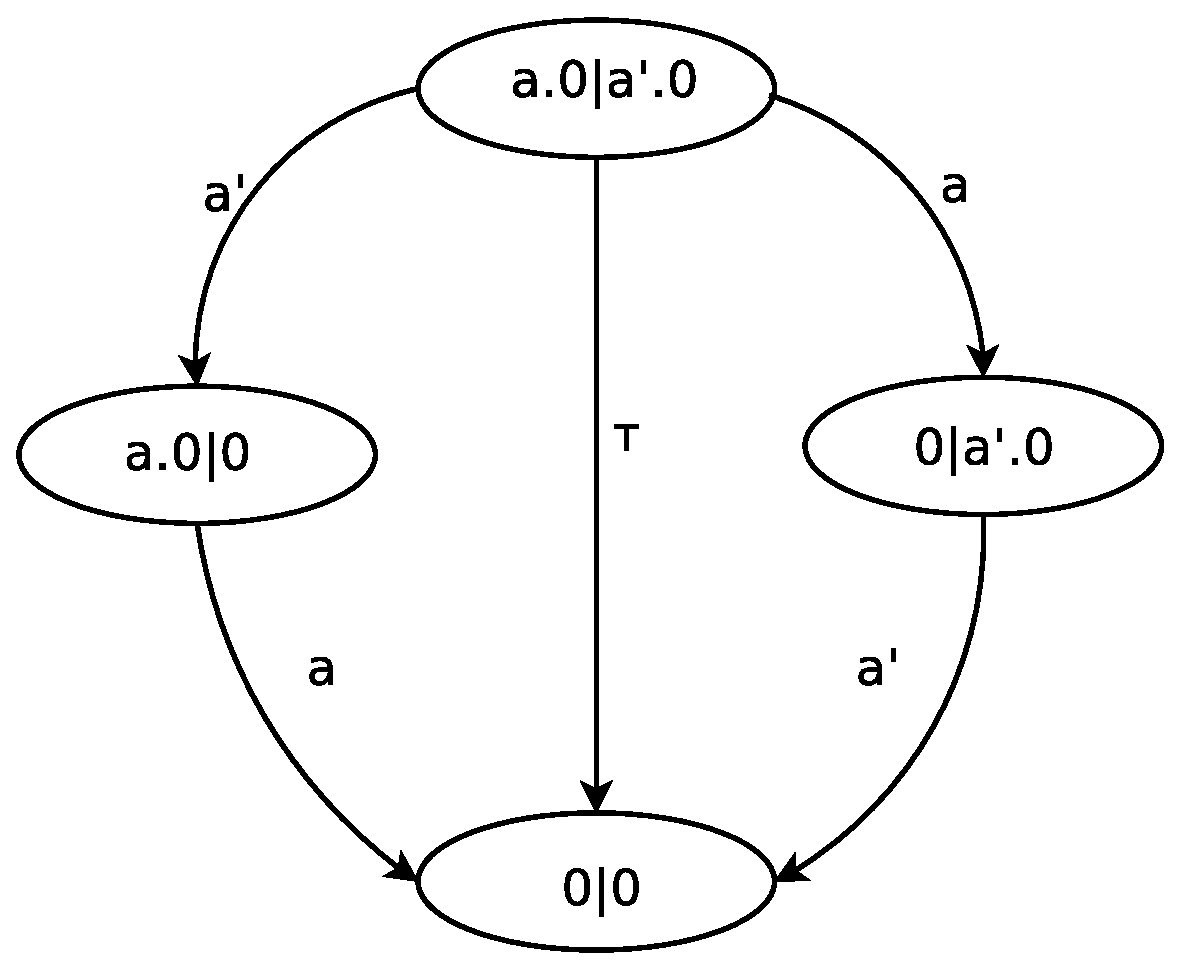
\includegraphics[scale=0.5]{graph1}
  \caption{Graph of $a.0 \mid \overline{a}.0$}
  \label{fig:graph1}
\end{figure}

This is illustrated in Fig. \ref{fig:graph1}.  To make the derivation
of $E|F$ deterministic, the scope of $a$ can be restricted.  In CCS,
an action or co-action can be paired with any complementary action
which is within its scope.  To force the input of $E$ to be paired
with the output of $F$ above, the scope of $a$ must be restricted so
as to include only $E$ and $F$.  This is handled by another operator
in the core syntax, $\backslash$.  Its operand $a$ is the name of a
channel whose scope is restricted to the process given as its left
operand.  So, in this case, $(E|F)\backslash a$ appropriately limits
the possible derivations to just $\derives{\tau}$.

The remaining binary operator is $+$, which provides non-deterministic
choice between two processes.  While the parallel composition operator
represents two processes running in parallel, $+$ corresponds to the
familiar idea of branching found in sequential models.  $E$ and $F$
thus represent two possible behaviours which may or may not occur.
Using the same two exemplar processes again, $E + F$ may derive as
follows:

\begin{enumerate}
\item $E\ +\ F \derives{a} E'$
\item $E\ +\ F \derives{\overline{a}} F'$
\end{enumerate}


\begin{figure}  
  \centering
\[
\xy
(20,0)*{a.E' \mid \overline{a}.F'}="1";
(0,-15)*{F'}="2";
(40,-15)*{E'}="3";
{\ar@/^2pc/^{a} "1";"3"};
{\ar@/_2pc/_{\overline{a}} "1";"2"};
%{\ar@/^2pc/^{\overline{a}} "3";"4"};
%{\ar@/_2pc/_{a} "2";"4"};
%{\ar^{\tau} "1";"4"};
\endxy
\]
%  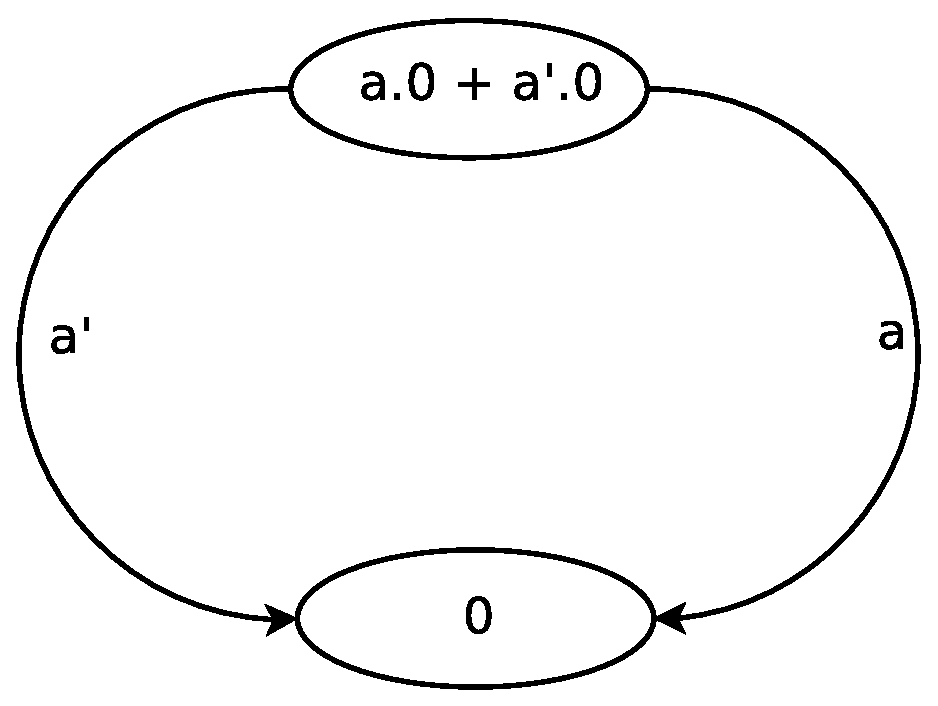
\includegraphics[scale=0.5]{graph2}
  \caption{Graph of $a.0 + \overline{a}.0$}
  \label{fig:graph2}
\end{figure}

Again, this is illustrated in Fig. \ref{fig:graph2}.  There are
clearly similarities between the possible derivations from $E|F$ and
$E+F$, but with choice, there is no possibility of synchronisation and
only one of the two transitions, $a$ and $\overline{a}$ is ever
performed.  The other is lost after the process makes its decision,
whereas with composition, it is possible to perform both actions, one
after the other.

The remaining operators in CCS handle recursion and relabelling.  The
process $\mu X.E$ binds $X$ to $E$, so that later occurrences of $X$
are replaced with $E$.  For example, $\mu X.a.X$ can perform an $a$
transition to become $\mu X.a.X$ again.  The function, $f$, in $E[f]$
has the type $\names \rightarrow \names$ and is used to rename actions
and their complements.  For example, $a.\overline{a}.\tau.0[a
  \rightarrow b]$ is $b.\overline{b}.\tau.0$.

An operational semantics for CCS can be given in terms of a labelled
transition system, $(\procs, \actions, \rightarrow)$, where $\procs$
is the set of CCS expressions formed from the above syntax, $\actions$
is as defined above and $\mathop{\rightarrow} \mathrel{\subseteq}
\procs \times \actions \times \procs$ is the transition relation
defined in Table \ref{tab:ccssemantics}.  We use $E$ and $F$ to range
over process terms ($\procs$), $\alpha$ over the set of actions
($\actions$), $\sigma$ over the set of clocks ($\timers$), $a$ and $b$
over the set of names ($\names$) and and $\gamma$ over $\names \cup
\timers$.

\begin{table}
  \caption{CaSE Semantics}
 \label{tab:ccssemantics}
  \shrule
 \vspace{-2mm}
 \begin{center}
 \begin{tabular}{rlrl}
     \Rule{Act}
     {-}
     {\alpha . E \derives{\alpha} E}
     {}
     &
     \Rule{Sum1}
     {E \derives{\alpha} E^\prime}
     {E + F \derives{\alpha} E^\prime}
     {}
     \\[3ex]
     \Rule{Sum2}
     {F \derives{\alpha} F^\prime}
     {E + F \derives{\alpha} F^\prime}
     {}
     &
     \Rule{Par1}
     {E \derives{\alpha} E^\prime}
     {E \;|\; F \derives{\alpha} E^\prime \;|\; F}
     {}
     \\[3ex]
     \Rule{Par2}
     {F \derives{\alpha} F^\prime}
     {E \;|\; F \derives{\alpha} E \;|\; F^\prime}
     {}
     &
      \Rule{Par3}
      {E \derives{a} E^\prime,
        F \derives{\overline{a}} F^\prime}
      {E \;|\; F \derives{\tau} E^\prime \;|\; F^\prime}
      {}
     \\[3ex]
      \Rule{Rec}
      {E \derives{\alpha} E'}
      {\mu X.E \derives{\alpha} E' \{ \mu X.E / X\}}
      {}
      &
      \Rule{Res}
      {E \derives{\alpha} E'}
      {E \res{b} \derives{\alpha} E' \res{b}}
      {\alpha \ne b}
      \\[3ex]
      \Rule{Ren1}
      {E \derives{a} E'}
      {E[f] \derives{f(a)} E'[f]}
      {}
      &
      \Rule{Ren2}
      {E \derives{\overline{a}} E'}
      {E[f] \derives{\overline{f(a)}} E'[f]}
      {}
 \end{tabular}
  \end{center}
  \shrule
\end{table}

\subsection{The Dining Philosophers}

To fully appreciate CCS, it is necessary to see how it may be used to
model an example scenario.  

Dijkstra's classic `Dining Philosophers' problem
\cite{dijkstra:philosophers} illustrates further issues which may
arise in a situation where multiple processes must interact to achieve
their goal.  In this scenario, five philosophers are seated around a
table, each with a plate of spaghetti and a fork.  The philosophers
divide their time between thinking and eating.  In order to eat, a
philosopher must obtain two forks, necessitating some form of
interaction.  This is a common situation in concurrency, where
multiple parallel processes (the philosophers) need to gain access to
shared resources (the forks).

In cases where things go awry, deadlock or starvation may result.  For
example, if all the philosophers simultaneously pick up the forks on
their left, then none of them will be able to eat; they will all end
up waiting for a fork held by another philosopher.  The system is said
to be \emph{deadlocked}, as none of the processes can obtain a lock on
the resource it needs, as a lock is already held by one of the other
processes\footnote{The solution to breaking this deadlock is to break
  the symmetry; if the fifth philosopher tries to take the fork on the
  right first, he or she will be unable to proceed, but the first
  philosopher will, using the fifth philosopher's left fork.}.
Alternatively, \emph{starvation} may result (literally in this case)
if one of the philosophers never stops eating and consequently never
releases the forks; the resources are unfairly distributed to the
deficit of one of the processes.

Modelling this in CCS involves first ascertaining which processes form
the basis of the system.  Clearly, each philosopher plays a part, so
they should be represented by processes.  Returning to the original
definition of the problem, each philosopher may choose to eat or
think.  In CCS, this can be represented as:

\begin{equation}
Philosopher = Eating + Thinking
\end{equation}

\noindent where the philosopher is recursively defined as making the
choice between $Eating$ or $Thinking$.  Defining the latter is simple;
thinking is simply some internal process of the philosopher:

\begin{equation}
Thinking = \tau .Philosopher
\end{equation}

The focus of the model is on the eating process, which requires access
to the system's shared resources: the forks.  Modelling this
necessitates defining a protocol whereby the philosopher may interact
with the resource in order to obtain access to it.  

\begin{equation}
Eating = \overline{take}.\overline{take}.\tau.\overline{replace}.\overline{replace}.Philosopher
\end{equation}

\noindent which needs to synchronize with two available forks if the
philosopher is to be able to eat (represented by $\tau$) and then
replace the forks again.  It follows that the forks must also be
represented using the process

\begin{equation}
Fork = \mu X.take.Fork^\prime
\end{equation}

\noindent with two communication channels, $take$ and
$replace$.  The fork begins its life on the table from which it
may be \emph{taken}, represented here by the receipt of an input on
the $take$ channel.  Once this has occurred, the process becomes

\begin{equation}
Fork^\prime = replace.X
\end{equation}

\noindent which represents the state where the fork is in use by a
philosopher.  The fork can't be used again until it has received an
input on $replace$, which causes $X$ to be expanded and the fork to
wait for input on $take$ again.

  The system as a whole is modelled by running a number of
  philosophers and forks in parallel, and restricting the scope of the
  fork channels in order to enforce synchronisation.

%\begin{figure}  
%  \centering
%  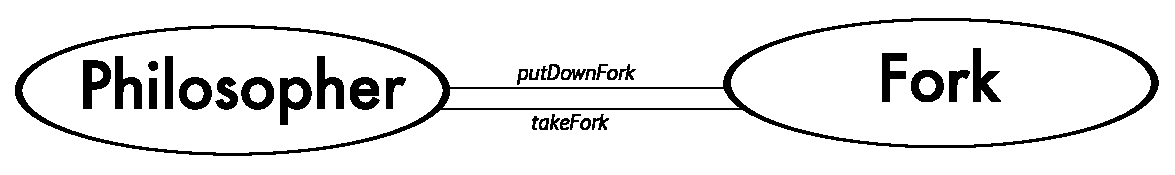
\includegraphics[scale=0.5]{philosophers}
%  \caption{The Dining Philosophers in CCS}
%  \label{fig:dpccs}
%\end{figure}

Note that this CCS representation of the problem only models the
narrative version of the problem above.  There is no attempt to
resolve any of the competition problems, and a strong element of
non-determinism, as to which philosopher gets which fork, still
exists.  It does, however, give a formal representation of the problem
and allows the effects of varying the relative numbers of philosophers
and forks to be observed via execution of the model.

Modifying this slightly gives a model that corresponds
exactly to a specified number of philosophers and forks, $n$.  From
the definitions above, multiple variants may be generated, such that
each philosopher and fork process has a unique subscript.  For
example, $Philosopher$ becomes $Philosopher_i$, where $i = 1\dots n$.
The same subscripting also applies to the $take$ and $replace$
channels, so that they now correspond to a specific fork.  The
original solution can thus be represented, as the case where each
$Philosopher_i$ initially performs the action $take_i$ (to take
the left fork) and then $take_{i-1}$ (with the exception that when
$i-1 = 0$, we use $n$)\footnote{Again, it is necessary to reverse the
  actions of $Philosopher_n$ in order to obtain a solution that does not
  deadlock.}.

This model restricts which fork is taken by which philosopher
(limiting the possible actions, and thus removing some
non-determinism), but is still prone to questions of non-deterministic
choice (some philosophers may arbitrarily choose to think instead) and
fairness, with regards to action performance (if the actions are
performed in a depth-first manner\footnote{i.e. if an implementation
  always chooses to execute a particular philosopher's choices
  first.}, only one philosopher may end up eating).  These may be
regarded as implementational aspects of the model.

\section{Advantages and Limitations of CCS}
\label{ccslimit}

From its syntax, it is clear that CCS can model sequential behaviour
using sequential composition ($\alpha.E$), non-deterministic choice
($+$) and $\nil$.  This further confirms the intuition noted earlier that
sequential programs are a subset of the larger set of concurrent
programs.  This is illustrated by the $+$ operator, which
returns a smaller set of possible derivations, from the same initial
pair of processes, when compared with parallel composition ($|$).
These sequential operators can also be used to convert a set of
parallel-composed processes into their equivalent interleavings.

CCS can model both sequential and concurrent programs, while still
maintaining a minimal syntax.  A finite axiomatisation can even be
defined, if the simultaneous presence of parallel compositon and
recursion is avoided \cite{milner:ccsaxiom}.  However, one fairly
obvious limitation is that there is no data in the model.  The
processes discussed so far don't explicitly communicate anything when
they send or receive signals.  Instead, behaviour arises purely from
synchronisation.  It is possible to extend CCS to represent this by
adding the concept of value passing between processes.  A host of
other process calculi have been based on such a variant of CCS, and we
will consider this in more detail as part of chapter \ref{mobility}.

CCS models are also relatively static; while processes may evolve
(e.g. $a.P$ may become $P$), the communication structure doesn't.
Notably, if a process, $E$ knows about the channels $x$ and $y$
initially, while $F$ only knows about $x$ (due to restriction on $y$),
this status can not change during the course of the various
transitions inherent in the system.  The effect of restriction is more
generally known as \emph{scoping} and occurs frequently with reference
to variables in programming languages.  CCS doesn't allow dynamic
changes to the scoping of channels.  Instead, scoping is fixed to the
static arrangement provided by the initial system, prior to any
transitions.  The addition of dynamic scoping, often referred to as
mobility, is the major contribution of the $\pi$ calculus, a language
based on CCS covered in \ref{scopemobility}.

To conclude, there is another limitation of CCS which is less to do
with a particular concept being absent from the language, instead
being more related to its central aspect: \textbf{synchronisation}.
The problem here lies in the \emph{compositionality} of processes.
While the structure of a CCS system remains compositional, because the
result of parallel composition is determined by the behaviour of the
composed processes together with the rules of the $|$ operator, this
is not true of the synchronisation of arbitrarily many processes.

Consider broadcasting a signal to an arbitrary number of processes.
Ideally, a general \emph{broadcast agent} should be defined which
provides this behaviour.  In CCS, there are at least two ways of
defining semantics for the agent, but not one that provides a suitably
compositional solution.  Perhaps the most obvious is simply to extend
the familiar synchronisation of two processes.  An input and output
pair can synchronize, so why not just create multiple pairs, one for
each receiving process?  For example, transmitting a signal to two
processes can be written simply as

\begin{equation}
\mathbf{\overline{a}_1.\overline{a}_2.0}\ |\ a_1.P\ |\ a_2.Q
\end{equation}

\noindent where the process on the left (in bold) forms the semantics
for the broadcast agent and the processes, $P$ and $Q$ are the
continuations of the input processes

This will work, but what happens when the broadcast agent needs to
transmit the signal to three processes?

\begin{equation}
\mathbf{\overline{a}_1.\overline{a}_2.\overline{a}_3.0}\ |\ a_1.P\ |\ a_2.Q\ |\ a_3.R
\end{equation}

\noindent The semantics of the broadcast agent have to change.  Simply
composing the third input will lead to one of the three being ignored
by the original definition of the broadcaster given above.  So, simply
enumerating multiple synchronisation pairs is not sufficient to
provide a compositional broadcast agent.

A second solution lies in recursion.  If the problem with the previous
solution lies in the broadcasting agent doing too little (i.e. not
transmitting to all the possible receivers), then, by making it
recurse, it will keep sending the output to whoever will synchronize
with it.  Thus, the example for three inputs above becomes

\begin{equation}
\mu X.\overline{o}.X\ |\ o.P\ |\ o.Q\ |\ o.R
\end{equation}

\noindent which works, and will continue to do so if a further
input process is parallel composed.  

But there is still a problem for much the same reasons as the first
solution.  This works fine on this small scale, but what happens when
this agent is placed in the context of a larger system?  Once the agent
starts its cycle of outputs, it won't stop as there exists
no base case for this recursion\footnote{A base case may be introduced
using non-deterministic choice, but there is no guarantee when this will
be invoked, if ever.}.  An output on $o$ will always be available (within
the scope of any restriction placed on that particular channel) and
the broadcasting process can never do anything else.  The result is a
constantly cycling process, which, in an implementation of this model,
would continue to consume resources.

The true solution to this problem is to enable some form of
\emph{global synchronisation}.  This requires a separate entity,
distinct from the processes involved in the communication, which can
be used to co-ordinate the synchronisation.  In the next chapter, a
branch of process calculi is considered which provides just such a
facility.

\section{Conclusion}

In conclusion, this chapter has taken a brief look at the field of
concurrency modelling, largely from the perspective of process
calculi.  Initially, it was shown that, while universal Turing
machines and the $\lambda$ calculus can simulate any recursive
function, their inherent sequential behaviour makes them unsuitable
for modelling concurrent systems.  CCS, in contrast, can model this
kind of behaviour and in a succient manner.  However, its minimal
syntax also leads to some limitations.  In the next two chapters, we
will look at some more process calculi, many of which use CCS as their
basis, and observe the benefits of features such as global
synchronisation (see chapter \ref{globsync}) and mobility (see chapter
\ref{mobility}).






% Thesis: Global Synchronisation
% Author: Andrew Hughes

\chapter{Global Synchronisation}
\label{globsync}

\section{Introduction}
\label{timing}

Initially, the use of the word `timed', within the context of the
calculi considered here, is a bit of a misnomer.  The notion of `time'
is generally associated with concrete real values, in units such as
minutes and seconds.  Real-time process calculi, such as those
described in \cite{aceto:timing, beaten:timing, brics:lee,
  lee:realtime, tccs, satoh:phd, satoh:distrib}, attempt to model
this.  Instead, this section focuses on a series of discrete timed
calculi which focus on abstract time and the use of \emph{clocks} for
the primary purpose of global synchronisation (as described above).

\section{Temporal Process Language (TPL)}
\label{tpl}

Hennessy's Temporal Process Language (TPL) \cite{hennessy:tpl} extends
the CCS language discussed above with a single clock, akin to a
hardware clock which emits a signal at an arbitrary point in time.
These signal emissions are controlled by a concept known as
\emph{maximal progress}, which allows each process to make as much
progress as possible before the clock ticks.  Formally, this means
that all silent actions ($\tau$s) are performed before a $\sigma$
action (which represents the clock signal) occurs.

This is of little use unless the actions of the processes can actually
depend on the behaviour of the clock.  The two are related via the
addition of a timeout operator.  This takes the form

\begin{equation}
\timeout{E}{\sigma}{F}
\end{equation}

\noindent where $E$ and $F$ are processes and $\sigma$ is the clock.  In
short, $F$ acts if $E$ \emph{times out} on the clock, $\sigma$.  This is
similar to non-deterministic choice, in that only one of the two
processes will ever act and the behaviour of the other is lost.  Here,
however, the choice is determined by the clock (and thus effectively by
the other processes, as it is their behaviour which controls when the
clock will tick).

With these additions, the problem of defining a suitable compositional
broadcast agent, as mentioned in \ref{ccslimit}, can be solved.
Recall the second solution, which used recursion.  Now, with the
addition of an external entity (the clock) and a way of relating it to
the processes involved (timeouts), a base case may be provided via
recognition of the point when no more synchronisations may occur.
This can be added to the earlier recursive solution

\begin{equation}
\mu X.\timeout{\overline{o}.X}{\sigma}{0}\ |\ o.P\ |\ o.Q\ |\ o.R
\end{equation}

\noindent by simply adding a timeout which stops the recursion.  This
works because the synchronisations of the input processes with the
output of the broadcast agent generate silent actions and thus invoke
maximal progress.  While there is a choice between a silent action
(due to the broadcasting agent synchronising with an input) and a
clock tick, the silent action always takes precedence and thus every
possible synchronisation occurs.  Once no more synchronisations are
possible, the clock is allowed to tick and the recursion stops.

\section{Extending TPL}
\label{tplext}

The extensions to TPL considered here focus on expanding the
scalability of the language.  As demonstrated above, TPL adequately
provides for situations where an arbitrary number of processes must
synchronize.  But what happens when a solution, like the one above, is
integrated into a larger system?  With only one clock, further
problems occur.  The use of the clock in one subsystem may conflict
with its use in another, and there is no clock available to
co-ordinate the subsystems themselves.

The Calculus for Synchrony and Asynchrony (CSA) \cite{csa} extends TPL
with the idea of multiple clocks, drawn from PMC\footnote{PMC also
  differs from TPL in its use of \emph{insistent} actions; all must be
  performed before a clock tick.}\cite{pmc}. However, while having
multiple clocks allows the use of differing patterns of
synchronisation, it increases the number of clock ticks present within
the system.  With five clocks, even the nil process has five possible
transitions (as clocks idle over nil).

CSA solves this to a limited extent by localising maximal progress to
a pre-defined scope for each clock.  A more elegant solution is
provided in the Calculus for Synchrony and Encapsulation (CaSE)
\cite{CaSE}, which introduces a clock hiding operator into the syntax.
The effect of this is the introduction of \emph{synchronous
  encapsulation}, as hidden clocks emit $\tau$ actions (as opposed to
ticks) outside the operator's scope.  This can be used, in conjunction
with restriction, to produce a hierarchy of components.  The actions
of these subsystems can be represented purely as silent actions, and,
when combined with the global form of maximal progress introduced by
TPL and retained in CaSE, integrated into the `synchronous cycle'
\cite{CaSE} of clocks at the level above.

\section{The Calculus of Synchronous Encapsulation (CaSE)}
\label{case}

The syntax for CaSE, given in \cite{norton05alg}, is as follows:
\begin{equation}
  \begin{aligned}
    \expr, \exprb\ ::=\ &
    \nil  \;\,|\,\; 
    \Delta \;\,|\,\; 
    \Delta_{\sigma} \;\,|\,\; 
    \alpha . \expr  \;\,|\,\;
    \expr + \exprb \;\,|\,\; 
   \expr \mathrel{\!|\!} \exprb \mid
    \timeout{\expr}{\sigma}{\exprb} \;\,|\,\; \\
    & \stimeout{\expr}{\sigma}{\exprb} \;\,|\,\; 
    \mu X . \expr \;\,|\,\; 
    X \;\,|\,\; 
    \expr \setminus a \;\,|\,\; 
    \expr / \sigma
  \end{aligned}
\end{equation}
where $\expr$ and $\exprb$ define possible process terms. We assume a
countable set of actions, $\actions = \names \cup \conames \cup
\{\tau\}$, ranged over by $\alpha$, where the elements of $\names$ are
drawn from an infinite set of \emph{names}, and $\conames$ is the
corresponding set of \emph{co-names}, $\{\overline{a} \mid a \in
\names\}$. $\timers$ is a countably infinite set of \emph{clocks} over
which $\sigma$ ranges. $X$ ranges over a countably infinite set of
variables, which are used to bind process behaviour in recursive
process definitions. $\nil$, $\alpha . \expr$, $\expr + \exprb$,
$\expr \mathrel{\!|\!} \exprb$, $\mu X . \expr$, $X$ and $\expr
\setminus a$ retain their behaviour defined in CCS, but now exhibit
additional actions due to the presence of clocks.

There are now transitions for the $\nil$ process, as, while the
process has no explicit behaviour, it can idle over the ticks of the
clocks.  This also applies to actions in general:

\begin{equation}
a.0 \derives{\sigma} a.0
\end{equation}

\noindent assuming a clock context containing just the one clock,
$\sigma$. Similarly, non-deterministic choice and parallel composition
exist through time, so both sides can evolve due to a clock tick,
while the operator remains in place.  This gives the following
possible derivations for $a.0\;|\;b.0$ (where $b \ne \overline{a}$):

\begin{enumerate}
\item $a.0\ |\ b.0 \derives{a} 0\ |\ b.0$
\item $a.0\ |\ b.0 \derives{b} a.0\ |\ 0$
\item $a.0 |\ b.0 \derives{\sigma} a.0\ |\ b.0$
\end{enumerate}

\noindent with the same clock context as above.  The third derivation
is duplicated for each available clock that can tick over both sides
of the composition.  In cases where both sides may synchronize,
causing a $\tau$ transition, this takes precedence over the clock
transitions, due to \emph{maximal progress} (see \ref{timing}) and the
original set of derivations for parallel composition (see \ref{ccs})
are available instead.

The changes to non-deterministic choice are simpler, as the operator itself
does not generate silent actions.  So, if both sides allow the clock to tick,
then the following derivations will occur:

\begin{enumerate}
\item $a.0\ +\ b.0 \derives{a} 0$
\item $a.0\ +\ b.0 \derives{b} 0$
\item $a.0\ +\ b.0 \derives{\sigma} a.0\ +\ b.0$
\end{enumerate}

\noindent again with the single clock, $\sigma$, as the context.

\subsection{Timeouts}

Moving on to the new operators, CaSE, as presented in
\cite{norton05alg}, includes two variants of the timeout operator,
first seen in TPL.  Recall from \ref{timing} that the operator
essentially allows a decision to be made, based on the presence of a
clock tick.  In the general scenario,

\begin{equation}
\timeout{E}{\sigma}{F}
\end{equation}

\noindent $F$ will act if $E$ fails to, prior to a clock tick.  If $E$
can perform a $\tau$ action, then this will prevent the clock tick and
$E$ will evolve. Both operators in CaSE maintain this core behaviour,
which is central to the concept of global synchronisation explained
earlier.

The difference between the two operators in CaSE lies in their
behaviour with regard to other clocks.  With the fragile timeout,
$\timeout{E}{\sigma}{F}$, any possible transition on $E$ will cause the
removal of the timeout.  So, with $\timeout{a.0}{\sigma}{b.0}$ and a clock
context of $\sigma$ and $\rho$, the following derivations can occur:

\begin{enumerate}
\item $\timeout{a.0}{\sigma}{b.0} \derives{a} 0$
\item $\timeout{a.0}{\sigma}{b.0} \derives{\sigma} b.0$
\item $\timeout{a.0}{\sigma}{b.0} \derives{\rho} a.0$
\end{enumerate}

\noindent where both the $a$ and the $\rho$ transition leave only the
left-hand side of the timeout.

The stable timeout differs by continuing to exist through time until
some action occurs.  While it exhibits the same behaviour in response
to actions or the tick of the specified clock, the ticks of other
clocks only cause the left-hand side to evolve; the timeout itself is
retained.  Thus, $\stimeout{a.0}{\sigma}{b.0}$ gives a different set
of derivations:

\begin{enumerate}
\item $\stimeout{a.0}{\sigma}{b.0} \derives{a} 0$
\item $\stimeout{a.0}{\sigma}{b.0} \derives{\sigma} b.0$
\item $\stimeout{a.0}{\sigma}{b.0} \derives{\rho} \stimeout{a.0}{\sigma}{b.0}$
\end{enumerate}

\noindent where the $\rho$ transition no longer causes the dissolution
of the timeout.

\subsection{Clock Stopping and Insistency}
\label{clockcontrol}

The remaining operators further control the behaviour of the clocks.
$\Delta$ prevents all clocks from ticking, while $\Delta_{\sigma}$
prevents only the ticks of the specified clock, $\sigma$.  $\Delta$ is
similar to the CCS version of $\nil$, as it has no possible
transitions.  $\Delta_{\sigma}$ exhibits transitions for all other
clocks within the current context.  So, for a context containing both
$\sigma$ and $\rho$, $\Delta_{\sigma}$ has a single transition,

\begin{equation}
  \Delta_{\sigma} \derives{\rho} \Delta_{\sigma}
\end{equation}

\noindent which is replicated for any other clocks in the context,
which are not equal to $\sigma$.

The stopping of clocks is used to provide \emph{insistency}.  Normally,
a process $a.P$ has two possible derivations:

\begin{enumerate}
  \item $a.P \derives{a} P$
  \item $a.P \derives{\sigma} P$
\end{enumerate}

\noindent with a clock context containing only $\sigma$.  To ensure
that the first of these two derivations occurs, or, in other words, to
\emph{insist} that $a$ is performed before the next tick of the clock,
$\sigma$, $\Delta$ is used.  The semantics for an insistent prefix,
$\underline{\alpha}.P$, may be given as:

\begin{equation}
\seml \underline{\alpha}.P \semr \eqdef \alpha.P + \Delta 
\end{equation}

\noindent where the presence of $\Delta$ prevents a $\sigma$
transition from occurring on the right-hand side of the choice, and
thus for the choice as a whole (as both sides must move through time
simultaneously).  This leaves only one available action,
$\derives{a}$, as required.  Clearly, insistency relative only to one
particular clock may also be defined in a similar manner, using
$\Delta_{\sigma}$ instead.

\begin{equation}
\seml \underline{\alpha}_{\sigma}.P \semr \eqdef \alpha.P + \Delta_{\sigma} 
\end{equation}

While on the subject of derived syntax, it is also possible to define
a clock prefix, akin to the existing action prefix:

\begin{equation}
\seml \sigma.P \semr \eqdef \stimeout{\nil}{\sigma}{P}
\end{equation}

\noindent where the stable timeout ensures that the $\sigma.P$ will be
retained until $\sigma$ ticks, despite the ticks of other clocks.  As
the only transitions for $\nil$ are clock ticks, only a tick from
$\sigma$ will cause the process to evolve and become $P$.

The two notions of a clock prefix and insistency can then be combined
to give an insistent clock prefix:

\begin{equation}
\seml \underline{\sigma}.P \semr \eqdef \stimeout{\Delta}{\sigma}{P}
\end{equation}

\noindent which differs from a standard clock prefix by only ever
allowing the one transition, $\underline{\sigma}.P \derives{\sigma}
P$, whereas $\sigma.P$ allows an arbitrary number of transitions from
other clocks before this occurs.

\subsection{Encapsulation}

Clock hiding is used to provide scoping for the ticks of a
clock.  Take the following situation,

\begin{equation}
\label{clockhidingex}
  (P / \sigma)\;|\;Q
\end{equation}

\noindent where $/ \sigma$ hides the clock, $\sigma$, so that its
ticks may only be seen by $P$.  $Q$ instead sees a silent action each
time $\sigma$ ticks.  Such clock hiding is central to the
encapsulation of components present in CaSE.  When coupled with
restriction, components can be made to emit only silent actions from
the perspective of external processes.

An operational semantics for CaSE can be given in terms of a labelled
transition system, $(\procs, \actions \cup \timers, \rightarrow)$,
where $\procs$ is the set of CCS expressions formed from the above
syntax, $\actions$ and $\timers$ are as defined above and
$\mathop{\rightarrow} \mathrel{\subseteq} \procs \times (\actions \cup
\timers) \times \procs$ is the transition relation defined in Table
\ref{tab:casesemantics}.  We use $E$ and $F$ to range over process
terms ($\procs$), $\alpha$ over the set of actions ($\actions$),
$\sigma$ and $\rho$ over the set of clocks ($\timers$), $a$ and $b$
over the set of names ($\names$) and $\gamma$ over $\names \cup
\timers$.

\begin{table}
  \caption{Semantics}
 \label{tab:casesemantics}
  \shrule
 \vspace{-2mm}
 \begin{center}
 \begin{tabular}{rlrl}
     \Rule{Idle}
     {-}
     {\nil \lderives{\sigma} \nil}
     {}
     &
     \quad \Rule{Act}
     {-}
     {\alpha . E \derives{\alpha} E}
     {}
     \\[3ex]
     \Rule{Patient\quad}
     {-}
     {a.E \derives{\sigma} a.E}
     {}
     &
     \Rule{Stall}
     {-}
     {\Delta_{\sigma} \derives{\rho} \Delta_{\sigma}}
     {\rho \ne \sigma}
     \\[3ex]
     \Rule{Sum1}
     {E \derives{\alpha} E^\prime}
     {E + F \derives{\alpha} E^\prime}
     {}
     &
     \Rule{Sum2}
     {F \derives{\alpha} F^\prime}
     {E + F \derives{\alpha} F^\prime}
     {}
     \\[3ex]
     \Rule{Sum3}
     {E \derives{\sigma} E^\prime, F \derives{\sigma} F^\prime}
     {E + F \derives{\sigma} E^\prime + F^\prime}
     {}
     &
     \Rule{Par1}
     {E \derives{\alpha} E^\prime}
     {E \;|\; F \derives{\alpha} E^\prime \;|\; F}
     {}
     \\[3ex]
     \Rule{Par2}
     {F \derives{\alpha} F^\prime}
     {E \;|\; F \derives{\alpha} E \;|\; F^\prime}
     {}
     &
      \Rule{Par3}
      {E \derives{a} E^\prime,
        F \derives{\overline{a}} F^\prime}
      {E \;|\; F \derives{\tau} E^\prime \;|\; F^\prime}
      {}
     \\[3ex]
      \Rule{Par4}
      {E \derives{\sigma} E^\prime,
        F \derives{\sigma} F^\prime,
        E \;|\; F \nderives{\tau}}
      {E \;|\; F \derives{\sigma} E^\prime \;|\; F^\prime}
      {}
     &
      \Rule{FTO1}
      {E \nderives{\tau}}
      {\timeout{E}{\sigma}{F} \derives{\sigma} F}
      {}
     \\[3ex]
      \Rule{FTO2}
      {E \derives{\gamma} E^\prime}
      {\timeout{E}{\sigma}{F} \derives{\gamma} E^\prime}
      {\gamma \ne \sigma}
     &
      \Rule{STO1}
      {E \nderives{\tau}}
      {\stimeout{E}{\sigma}{F} \derives{\sigma} F}
      {}
     \\[3ex]
      \Rule{STO2}
      {E \derives{\alpha} E^\prime}
      {\stimeout{E}{\sigma}{F} \derives{\alpha} E^\prime}
      {}
     &
      \Rule{STO3}
      {E \derives{\rho} E^\prime}
      {\stimeout{E}{\sigma}{F} \derives{\rho} \stimeout{E^\prime}{\sigma}{F}}
      {\rho \ne \sigma}
     \\[3ex]
      \Rule{Rec}
      {E \derives{\gamma} E^\prime}
      {\mu X.E \derives{\gamma} E^\prime \{ \mu X.E / X\}}
      {}
      &
      \Rule{Res}
      {E \derives{\gamma} E^\prime}
      {E \res{a} \derives{\gamma} E^\prime \res{a}}
      {\gamma \ne a}
     \\[3ex]
     \Rule{Hid1}
     {E \derives{\sigma} E^\prime}
     {E / \sigma \derives{\tau} E^\prime / \sigma}
     {}
     &
     \Rule{Hid2}
     {E \derives{\gamma} E^\prime}
     {E / \sigma \derives{\gamma} E^\prime / \sigma}
     {\gamma \ne \sigma}
     \\
 \end{tabular}
  \end{center}
  \shrule
\end{table}

\section{Advantages and Disadvantages of Timed Calculi}
\label{timelimit}

The main advantage of the timed calculi we have discussed here is that
they allow, via the introduction of \emph{global synchronisation}, the
construction of systems on a larger scale than those that could be
created purely with CCS.  With CaSE, components can be created which
consist of multiple processes and clocks.  These can then be
successfully integrated together to form new components.

Global synchronisation allows the problem of defining a compositional
broadcast agent, cited earlier in \ref{ccslimit}, to be solved, but
these timed calculi still retain the other problems with CCS we
mentioned there.  Neither TPL, PMC, CSA nor CaSE explicitly include
data within the model.  This is not necessarily a disadvantage; it is
possible to model data implicitly, via the use of silent actions, and
including data in the model complicates formal reasoning and
equivalence theories.

More importantly, these calculi all still retain a static structure.
The scope of restriction or clock hiding doesn't change as the
processes evolve.  This prevents these calculi from being used to
model mobile systems where these elements do change, although they
are perfectly suited to modelling static dataflow-oriented systems
such as those in \cite{WICSA} and \cite{cashews-sem}.

In contrast, the following section contains a discussion of calculi
which, while lacking the scalability of the timed languages just
illustrated, can model \emph{mobile systems}.

\section{Conclusion}

Discrete timed calculi can overcome this.  An example using TPL to
model a compositional broadcasting agent, using semantics suitable for
any arbitrary number of processes, is provided in \ref{timing}.
Extensions to TPL, such as CaSE, may scale even further using
synchronous encapsulation to create systems of multiple components.

% Thesis: Mobility
% Author: Andrew Hughes

\chapter{Mobility}
\label{mobility}

\section{Introduction}

Within the field of algebraic process calculi, there are two clear ways
in which the dynamic nature of a system is modelled.  The most
well-known is the form of mobility present within Milner's $\pi$
calculus which allows the scope of a name to change as the system
evolves.  This concept can be thought of in a similar way to the
reference passing that occurs in most programming languages; part of the
program begins with no knowledge of an entity, and later gains knowledge
by obtaining a reference to it.

Models in the $\pi$ calculus are not really mobile in the sense of
something moving from one place to another.  This isn't possible, as
there is no real notion of `place' to begin with.  However, the addition
of this mechanism does allow the modelling of dynamic systems, such as a
mobile phone network \cite{milner:lecture}, and is sufficiently
expressive as to allow it to encode Church's $\lambda$ calculus
\cite{funcproc}.

A more naturalistic form of mobility is found in calculi which allow
entities to \emph{migrate}.  One of the primary exponents of this is
Cardelli and Gordon's ambient calculus \cite{amb}, which groups
composed processes inside \emph{ambients}.  These ambients can be
moved up and down a nested hierarchy of such objects, or destroyed.  The
calculus differs from those previously considered, in that it
lacks communication primitives.  Surprisingly, the base syntax is
sufficient to allow communication to be encoded within them, and
indeed the entire asynchronous form of the $\pi$ calculus can be
represented.

The following two sections consider examples of both types of mobile
calculi in more detail.
 
\section{Scope Mobility}
\label{scopemobility}

\subsection{The $\pi$ Calculus}
\label{picalculus}

The $\pi$ calculus follows on from Milner's earlier work on CCS
discussed in \ref{ccs}. Essentially, it is a value-passing form of CCS
in which values and channels are replaced simply by \emph{pure names}.
Thus, channels can be passed between processes, as well as values,
which means that their scope may change during execution.

To make this clearer, consider the syntax of the form of $\pi$ calculus
given in \cite{funcproc}

\begin{equation}
\label{pisyntax}
  E, F\ ::=\ 
  0\ |\ 
  \overline{x}y.E\ |\ 
  x(y).E\ |\ 
  (a)E\ |\ 
  (E\ |\ F)\ |\ 
  !E
\end{equation}
  
\noindent which is a minimal version containing replication as opposed
to recursion, with $a$ a channel name and $x$ and $y$ being defined
below.  Compare this with the syntax given for CCS in Eqn.
\ref{ccssyntax}.  The nil process, $0$, is still present, as is parallel
composition and restriction (although in a new form, $(a)E$).
Non-deterministic choice is present in the original version of the $\pi$
calculus presented in \cite{picalctutorial}, but is removed from the
version given in \cite{funcproc} due to the formulation of semantics
used there.  $!E$ is the syntax for replication, which replaces
recursion in this particular variant of the calculus to give a simpler
theoretical treatment, while still doing much the same job.

The main distinction between the two lies in the remaining element of
the syntax: prefixing.  In CCS, a more general syntax, $\alpha.E$,
where $\alpha \in \mathcal{N} \cup \overline{\mathcal{N}} \cup
\{\tau\}$, is used and includes input, output and silent actions.  In
the syntax given above for the $\pi$ calculus, the input ($x(y)$) and
output ($\overline{x}y$) syntax are given separately, and the input
prefix is \emph{binding}\footnote{When an input is received on $x$,
  $y$ is bound to the value of that input, which is then substituted
  for $y$ in the continuation of that process.} like restriction. $x$
and $y$ are both names, where `$x$ [is] the \emph{subject} and $y$ the
\emph{object}' \cite{funcproc}.  Silent actions no longer appear in
prefix form, but do occur as $\tau.E$ in some variants of the $\pi$
calculus.

The distinction between the $\pi$ calculus and value-passing forms of
CCS, which also use this form of prefixing, lies in $x$ and $y$ being
drawn from the same set in the $\pi$ calculus.  In contrast,
value-passing forms of CCS keep the two sets distinct, so that the
channel and value names do not intersect.  This change is what
gives $\pi$ calculus its power, as channels can now be used as the
object of an input or output.  Thus,

\begin{equation}
x(y).\overline{y}x.0
\end{equation}

\noindent becomes perfectly valid.

This also has an effect on restriction.  Recall that, in CCS,
$(a.0|\overline{a}.0)\backslash a$ restricts the scope of $a$ to just
the two processes, $a.0$ and $\overline{a}.0$, making a synchronisation
the only possible action which may be performed.  Now consider the
following processes defined using the $\pi$ calculus:

\begin{equation}
(a)(a(x).\overline{x}a.0\;|\;\overline{a}y.0)\;|\;y(z).P
\end{equation}

\noindent where the scope of $a$ is again restricted, this time to the
two processes $a(x).\overline{x}a.0$ and $\overline{a}y.0$.  If these
two processes synchronize, the system evolves to:

\begin{equation}
(a)(\overline{y}a.0\;|\;0)\;|\;y(z).P
\end{equation}

\noindent with $x$ becoming bound to the channel name, $y$.  This shows
how the $\pi$ calculus allows channel names to be passed between
processes, but it is the next transition that is really interesting.
$\overline{y}a.0$ will pass the channel name, $a$, to $y(z).P$, which is
outside the scope of the restriction imposed on $a$.  As a result, the
scope of $a$ is \emph{extruded}:

\begin{equation}
(a)(0\;|\;0\;|\;P\{a/z\})
\end{equation}

\noindent so as to include the process, $P$, in which $a$ is now
substituted for $z$.  Further, one of the structural congruence rules of
the $\pi$ calculus \cite{funcproc}:

\begin{equation}
(x)(P\;|\;Q) \equiv P\;|\;(x)Q\text{ if x not free in P}
\end{equation}

\noindent may be used to perform \emph{scope intrusion}, giving:

\begin{equation}
0\;|\;0\;|\;(a)(P\{a/z\})
\end{equation}

\noindent as the channel $a$ no longer occurs in the other two
processes.  These changes in scope are central to the concept of
mobility within the $\pi$ calculus.  They reflect the dynamic
environment of the processes represented, and give the calculus a
greater expressivity.

\subsection{Variants of the $\pi$ Calculus}
\label{pivariants}

Multiple variants of the $\pi$ calculus exist, including various
evolutions of the syntax and semantics.  As noted above, replication
is only introduced in the version of the calculus given in
\cite{funcproc}, which also defines a reduction-based semantics.  The
earlier tutorial papers \cite{picalctutorial} instead use recursion
and a structured operational semantics, based on a labelled transition
system.

The polyadic $\pi$ calculus \cite{milner:93polyadic} is a more
distinct variant.  Essentially, this involves a syntactic change to
input and output, so that a tuple is used, as opposed to the single
names used in the monadic $\pi$ calculus\footnote{This is a term used
  to refer to the original $\pi$ calculus in retrospect.}.  Having
this as a core part of the syntax provides advantages in representing
abstractions and giving a natural sort discipline\footnote{Sorts are a
  way of applying typing to the $\pi$ calculus, which will be covered
  further in section \ref{typedcalculi} on typed calculi.}.  However,
it is also possible to simply provide an encoding of this in the
monadic variant.

Doing so is not simply a matter of transmitting each value in
sequence; the operation needs to respect the atomicity implicit in the
use of multiple names.  Observe the following example from
\cite{milner:93polyadic}:

\begin{equation}
x(yz)\;|\;\overline{x}y_1z_1\;|\;\overline{x}y_2z_2
\end{equation}

\noindent where the process on the left should receive either $y_1$ and
$z_1$ or $y_2$ and $z_2$.  With the following semantics,

\begin{align}
\seml x(yz) \semr & \eqdef x(y).x(z) \\
\seml \overline{x}yz \semr & \eqdef \overline{x}y.\overline{x}z
\end{align}

\noindent the two sending processes can interfere with one another.
$y$ will become bound to either $y_1$ or $y_2$ on the first
synchronisation, which is fine, but $z$ may then receive whichever of
these two remains instead of the second element in the tuple.  This
happens because there is no link between the two synchronisations.
Thus, each subsequent transmission results in a new competition
between the two processes as to who actually synchronises with the
receiver.

The solution to this problem is to make use of a \emph{private
  channel}.  Before transmitting any of the names that form part of
tuple, the sending process passes a reference to a new channel to the
receiver.  The receiver then uses this channel to receive the contents
of the tuple, rather than relying on an existing channel, which may be
prone to interference.  Thus, the semantics become:

\begin{align}
\seml x(yz) \semr & \eqdef x(w).w(y).w(z) \\
\seml \overline{x}yz \semr & \eqdef (w)(\overline{x}w.\overline{w}y.\overline{w}z)
\end{align}

\noindent where $w$ is the new private channel created to facilitate
the process of transmitting the tuple.  This ability to encode the
polyadic variant in the original monadic calculus implies that the new
syntax fails to yield any greater expressivity, but this is not really
the motivation behind this extension.  Instead, what this provides is
a more natural way of transmitting information, which makes modelling
relatively complex systems easier.

The asynchronous $\pi$ calculus
\cite{boudol:asynchrony,honda:asynchronouscommunication,sangiorgi:asynchronousprocesscalculi}
deliberately reduces the level of expressivity in order to simplify
reasoning and provide a better framework for distributed
implementations.  The output prefix, $\overline{x}y.E$ is replaced
with $\overline{x}y.0$, so that there is no continuation after an
output.  In the original synchronous $\pi$ calculus, the behaviour of
the continuation, $E$, is blocked until a synchronisation with a
recipient can occur.  This doesn't occur in the asynchronous variant,
as there is no longer any behaviour dependent on this output
occurring.

  Synchrony can be emulated in the asynchronous polyadic $\pi$
  calculus, just as synchronous messaging frameworks, such as TCP, can
  be implemented on top of an asynchronous network.  The receiver
  simply has to acknowledge receipt of the message by replying to the
  sender.  The following semantics are given for the monadic prefixes
  in \cite{boxedamb01}:

\begin{align}
\seml \overline{c}x.P \semr & \eqdef (r)(\overline{c}xr\;|\;r.P) \\
\seml cy.P \semr & \eqdef c(yr).(\overline{r}\;|\;P)
\end{align}

\noindent where $r$ is not free in $P$ and $r.P$ is a syntactic
abbreviation for $r().P$ i.e. the input is an empty tuple.  The output
is encoded as the transmission of a tuple containing two names: $x$,
the original name being sent, and $r$, a new channel created to
receive the acknowledgement from the recipient.  This runs in parallel
with another process that awaits an input on $r$ before continuing
with $P$.  For example,

\begin{equation}
\begin{aligned}
& \overline{c}x.P \pc cy.Q \\
\equiv \quad & (r)(\overline{c}xr\;|\;r.P) \pc c(ys).(\overline{s}\;|\;Q) \\
\derives{} \quad & (r) (r.P \pc \overline{r} \pc Q\{x/y\}) \\
\derives{} \quad & P \pc Q\{x/y\}
\end{aligned}
\end{equation}

\noindent Thus, the original synchronous behaviour is emulated, as $P$
will not evolve until the receiver has obtained the private channel,
$r$, and replied.

Other changes to the calculus are also commonly adopted to reduce its
expressivity, thus making more proofs feasible.  These include:

\begin{itemize}
\item \emph{input localisation} \cite{merro:locality}, whereby a link
  received from another process can not be used for input.  For
  example, a process $a(x).P$ may not use $x$ as a channel upon which
  to receive input in $P$.
\item \emph{uniform receptiveness}
  \cite{sangiorgi:uniformreceptiveness}, where the input end of a link
  occurs only once syntactically and is replicated so as to be always
  available.
\item \emph{input-guarded replication}, which is not just restricted
  to uniform receptiveness variants, but is generally used as a more
  restricted form of replication (so the replication operator becomes
  $!a(x).P$ rather than $!P$).
\end{itemize}

The final variant of the $\pi$ calculus considered here is the
extension to higher-order operations.  The most obvious change to make
in this direction is to allow processes to be exchanged.  Such a
second-order form of the calculus is given by the \emph{Calculus of
  Higher Order Communicating Systems} (CHOCS) \cite{thomsen:chocs},
which actually predates the $\pi$ calculus itself.  This extended CCS
with mobility by allowing processes, rather than channel names, to be
transmitted.

The more general area of higher-order $\pi$ calculus, and the theory
behind it, is covered in Sangiorgi's thesis \cite{sangiorgi:phd}.  It
defines an extension to the $\pi$ calculus, HO$\pi$, which not only
allows the transmission of names (first-order) and processes
(second-order), but also parameterised processes of arbitrarily high
order ($\omega$-order).  This is best illustrated by some examples,
drawn from \cite{sangiorgi:phd}.  In the simplest case, an `executor'
process can be defined, $x(X).X$, which will receive and then execute an
arbitrary process.  Placing this in an appropriate context,

\begin{equation}
\overline{x}P.Q\;|\;x(X).X
\end{equation}

\noindent the process on the left, $\overline{x}P.Q$, will transmit
the process, $P$, to the executor before continuing as $Q$.  Thus,
following the synchronisation of the two processes, this system
evolves to become:

\begin{equation}
Q\;|\;P
\end{equation}

\noindent where the process $P$ having being substituted for $X$.  

A more complex example is given by considering Milner's encoding of
the natural numbers \cite{milner:93polyadic}.  A natural number, $n$,
is encoded as a series of outputs on $y$, the number of which is equal
to $n$ (represented as $\overline{y}^n$), followed by a transmission
on $z$ to indicate zero and thus, the end of the number:

\begin{equation}
\seml n \semr \eqdef (y,z)\overline{y}^n.\overline{z}
\end{equation}

\noindent Using HO$\pi$, the addition of these numbers can be encoded
in a very simple way.  In the $\pi$ calculus, summation is achieved
via an indirect reference to the two numbers, using channel names.  In
HO$\pi$, the parameterised processes or \emph{agents} that represent
the numbers can be used directly in the representation of addition.
Thus, actually adding the two numbers together becomes a simple matter
of running the two concurrently, and linking them via a common
channel.

A $Plus$ agent, which performs the addition of two numbers, can be
defined as follows:

\begin{equation}
Plus \eqdef (X,Y)(y,z)((x)(X\langle y,x\rangle \;|\;x.Y\langle y,z\rangle ))
\end{equation}

\noindent where both $X$ and $Y$ are agents with two parameters,
corresponding to $y$ and $z$ respectively in the definition of $\seml
n \semr$ above.  The operation of this agent is best demonstrated by
example.  Assume $X$ is two and $Y$ is three, represented in HO$\pi$ as:

\begin{align}
X(y,z) & \eqdef \overline{y}.\overline{y}.\overline{z} \\
Y(y,z) & \eqdef \overline{y}.\overline{y}.\overline{y}.\overline{z}
\end{align}

\noindent and retaining the same representation used for $\seml n
\semr$ above.  When $X$ and $Y$ are passed to the $Plus$ agent, $X$ is
instantiated with a new private channel, $x$, in place of $z$ in the
above.  $Y$ is then prefixed with an input on this same channel, so
that the $y$ outputs occurring in $Y$ only execute after those in $X$.
This leads to the following sequence of transitions:

\begin{equation}
  \lderives{y} \lderives{y} \lderives{\tau} \lderives{y} \lderives{y} \lderives{y} \lderives{z}
\end{equation}

\noindent which is close to the sequence that occurs for the
representation of five in HO$\pi$:

\begin{equation}
  \lderives{y} \lderives{y} \lderives{y} \lderives{y} \lderives{y} \lderives{z}
\end{equation}

Formally, the two are \emph{weakly bisimilar}.  A \emph{bisimulation} is
a symmetric binary relation between two processes, which exists if each
process can simulate the behaviour of the other.  $R$ is such a relation
iff, for all pairs of processes $(p,q)$ in $R$ and all actions,
$\alpha$\footnote{The bisimulation definition given here is more
applicable to the static systems of CCS.  Although it holds for this
simple example, a more detailed method of bisimulation is required to
handle the dynamic binding that occurs in the $\pi$ calculus and its
derivatives.}:

\begin{enumerate}
\item $P \derives{\alpha} P^\prime \implies \exists Q^\prime\ such\
  that\ Q \derives{\alpha} Q^\prime\ and\ (P^\prime,Q^\prime) \in R$
\item $Q \derives{\alpha} Q^\prime \implies \exists P^\prime\ such\
  that\ P \derives{\alpha} P^\prime\ and\ (P^\prime,Q^\prime) \in R$
\end{enumerate}

For a weak bisimulation, $\tau$ transitions are effectively ignored.
A series of such transitions,
$\derives{\tau}\derives{\tau}\derives{\tau}\dots$ is abbreviated to
$\obsderives{\tau}$ and $\obsderives{\tau} \derives{a}
\obsderives{\tau}$ is deemed equivalent to $\derives{a}$.  As the
additional $\tau$ transition in the $Plus$-based derivation is the
only difference between the two, the two can be deemed equivalent
under the rules of weak bisimulation.

Returning to HO$\pi$, the most interesting point about this calculus
is not that it provides the means to formulate abstractions of the
type just demonstrated, but that, in doing so, it adds no further
expressivity.  Indeed, Sangiorgi, in his thesis \cite{sangiorgi:phd}
demonstrates how a HO$\pi$ calculus can be represented in the $\pi$
calculus.  Thus, just as with the polyadic variant, the benefit of
using HO$\pi$ comes not from increased expressivity, but from the
additional ease it provides in modelling certain scenarios.

\subsubsection{The Join Calculus}
\label{join}

The Join calculus \cite{join} takes the asynchronous $\pi$ calculus as
its basis, and focuses on providing a formalism better suited as the
basis for a distributed implementation.

Take the following example of a $\pi$ calculus process given in
\cite{joinresults}:

\begin{equation}
x(y).P\;|\;x(z).Q\;|\;\overline{x}a
\end{equation}

\noindent where two processes are waiting to receive input on $x$.
The problem with implementing this in a distributed setting is that
there is no concept of location with the $\pi$ calculus.  Each of the
two receiving processes or \emph{receptors}\footnote{The join calculus
  uses an analogy with chemistry to describe its behaviour, based on
  the \emph{CHemical Abstract Machine} (CHAM) \cite{cham}.} may be
located at an arbitrary distance both from each other and from the
transmitter, $\overline{x}a$.  As a result, a \emph{distributed
  consensus problem} arises as to which of the two receptors will
receive the transmission.

The join calculus provides a solution to this problem by altering the
syntax of the $\pi$ calculus.  The asynchronous variant of the
syntax given in Eqn. \ref{pisyntax} becomes:

\begin{align}
\label{joinsyntax}
  P, Q\ & ::=\ 
  0\ |\ 
  \mathtt{def}\ D\ \mathtt{in}\ P\ |\
  (P\;|\;Q)\ |\ 
  x\langle \tilde{v} \rangle \\
  D, E\ & ::=\
  J \rhd P\ |\
  D \wedge E\ |\ 
  \mathbf{T} \\
  J,J^\prime\ & ::=\ 
  x\langle \tilde{v} \rangle\ |\
  (J\;|\;J^\prime)
\end{align}

\noindent with $\mathbf{T}$ being the empty definition and a clear
focus on linking the receptors in $D$ to the emissions occurring in $P$
(both represented by the same syntax, $x\langle \tilde{v} \rangle$).
The use of this is most clearly demonstrated by example:

\begin{equation}
  \mathtt{def}\ (x\langle y \rangle \rhd P) \wedge (x\langle z \rangle \rhd Q)\ \mathtt{in}\ x \langle a \rangle
\end{equation}

\noindent which has essentially the same behaviour as the $\pi$
calculus example presented earlier.  $x\langle y \rangle \rhd P$
receives an input, $y$, on $x$ and then continues as $P$.  $x\langle y
\rangle$ is said to guard $P$, and multiple such guards may be applied
to a single such process.  Multiple such receptors may be defined via
use of the $\wedge$ operator.

It is impossible to provide an exact equivalent to the earlier series
of $\pi$ calculus processes, as the changes in the join calculus now
prevent such scenarios from being created.  Instead, the equivalent of
this join calculus example in the $\pi$ calculus is:

\begin{equation}
(x)(!(x(y).P\;|\;x(z).Q)\;|\;\overline{x}a)
\end{equation}

\noindent where the scope of $x$ is restricted to the $\mathtt{def}$
expression and the inputs are replicated, so as to be always
available.  Thus, a channel $x$ is always \emph{localised} to a
particular set of emitters and receptors.

Clearly, the join calculus, as a reformulation of the asynchronous
$\pi$ calculus with a new syntax, can not be used to express anything
which can't be expressed in the $\pi$ calculus.  However, it has a lot
of advantages in endowing the calculus with distributive properties at
the syntactic level.\footnote{Such changes have also been made using the
restrictions imposed by an appropriate type system \cite{sangiorgi:uniformreceptiveness}.}

\subsection{Advantages and Disadvantages of the $\pi$ Calculus}

The $\pi$ calculus is a powerful formalism drawn from a minimal
abstract syntax.  As noted at the start of this section, it is capable
of encoding the $\lambda$ calculus and so it follows that it is also
capable of simulating any recursive function.

The problem is that this makes it a little too powerful in some cases.
From \cite{sangiorgi:types-or}, we can see how much more difficult the
additional power given by the $\pi$ calculus makes proving
termination.  In contrast, a sufficiently restricted form of CCS
provides a trivial proof.  In the same paper, Sangiorgi also touches
on something which seems common within the literature
\cite{join,failure2,wojciechowski:phd,stefani:kells}; while the
expressiveness of the $\pi$ calculus is interesting, it is necessary
to restrict it in order to actually have something which is generally
useful for reasoning over or using as the basis for a full programming
language.

Another problem with the $\pi$ calculus is that it carries with it a
trait from CCS.  Namely, it can't be used to model synchronisation
with an arbitrary number of processes in a compositional way.  This
was considered earlier in \ref{ccslimit} for CCS, and solved in
\ref{timing} using the additions to the calculus given by TPL.  While
the $\pi$ calculus has a notion of mobility and is thus more
expressive than CCS, it still lacks an external entity with which to
co-ordinate such a transaction.  

A common motif reoccurs here, that was touched on earlier in the
introduction to this review; even though something has a certain level
of expressivity, it doesn't follow that it is the most appropriate
mechanism for modelling a particular phenomenon.  This also holds for
the distributed calculi considered in \ref{migration}.  The $\pi$
calculus may already model mobility, but these calculi do so in a
different way, which may prove more suitable in a particular context.
 
\section{Distribution and Migration}
\label{migration}

Allowing the scope of a name to change during execution is one
possible way of modelling dynamic behaviour, but it isn't the only
way.  The concept of \emph{mobility} naively implies the physical
movement of processes, but, as shown above, this is not what actually
happens in the $\pi$ calculus.  To do so requires some notion of
\emph{distribution}; this can be provided by \emph{localities}, a term
used to refer generally to a higher-level form of grouping, above that
of processes.  This concept has been applied to various calculi, in
different forms, in order to model physical
sites~\citeaffixed{wojciechowski:phd}{Nomadic Pict,}, administrative
or security domains \citeaffixed{amb,seal}{the Ambient Calculus and
  the Seal Calculus,} and biological cells \citeaffixed{brane04}{Brane
  Calculi,}, but can theoretically be applied in any context where the
grouping of processes is useful.  Localities can be used simply for
observation or as a means to further control the behaviour of the
processes encapsulated within them.  They are generally named, so as
to provide a communication target or a known destination for a
migrating entity.

Originally, localities were used to distinguish between processes in
order to provide further equivalence theories.  Take the following simple
CCS-based example process:

\begin{equation}
\label{lccsspec}
Spec \eqdef in.\tau.\overline{out}.Spec
\end{equation}

\noindent which forms the \emph{specification} for the behaviour of a
system that receives an input, processes it and then returns the output.
The actual \emph{implementation} may differ from the specification by
instead involving two processes:

\begin{align}
\label{lccs2proc}
Receiver & \eqdef in.\overline{a}.Receiver \\
Sender & \eqdef a.\tau.\overline{out}.Sender
\end{align}

\noindent which communicate over another channel, $a$.  If these two
processes are run concurrently:

\begin{equation}
(Receiver\;|\;Sender)\setminus a
\end{equation}

\noindent with the scope of $a$ restricted, they are \emph{weakly
bisimilar} (see \ref{pivariants}) to one another.  The specification
performs the following derivations:

\begin{equation}
  \lderives{in} \lderives{\tau} \lderives{\overline{out}}
\end{equation}

\noindent prior to recursing and becoming $Spec$ again, whereas the
implementation produces:

\begin{equation}
  \lderives{in} \lderives{\tau} \lderives{\tau} \lderives{\overline{out}}
\end{equation}

\noindent with the extra $\tau$ transition caused by the synchronisation
on $a$.  As weak bisimulation effectively ignores $\tau$ actions, the
two are judged to be equivalent.  If the specification was to include a
further $\tau$ action, for an arbitrary reason, prior to the
$\overline{out}$, then the two would also be strongly bisimilar.  To
summarise, the difference between the two sets of derivations is
negligible, according to the bisimulation, yet the actual
difference between the specification and its implementation is fairly
significant.  The specification effectively requests a monolithic
solution, but weak bisimulation allows the final implementation to be
distributed over multiple processes.

In most situations, this is beneficial.  It means that the specification
can be met by a concurrent system, composed of multiple processes
running in parallel, superfluous $\tau$ transitions aside.  When a
distinction between the number of processes used is required, a finer
equivalence is needed.  \emph{Location bisimulation} \cite{obslocal}
provides exactly that, by assigning locations to processes and using
them as part of the relation between processes.

Essentially, this means that each transition is annotated with a
location name.  In \cite{obslocal}, a located variant of CCS is
defined, LCCS, which adds an additional piece of syntax, $l::E$ to
signify that a process $E$ is located at $l$.  This association is
made within the operational semantics, of which there are two
variants.  The \emph{static} approach allocates locations initially,
while the \emph{dynamic} method generates a new location for each
non-silent transition.  Here, the focus is on the latter, shown in
Table \ref{tab:lccssemantics}, which essentially gives each process a
\emph{causal path}, by explicitly representing the number of
transitions that have been performed.

\begin{table}
  \caption{LCCS Dynamic SOS Rules}
  \label{tab:lccssemantics}
  \shrule
 \begin{center}
    \begin{tabular}{lcr}
      \Rule{\textsf{Act1}}
      {-}
      {a . E \xrightarrow[l]{a} l::E}
      {for\ any\ l \in Loc}
      &
      \Rule{\textsf{Act2}}{E \xrightarrow[u]{a} E^\prime}
      {l::E \xrightarrow[lu]{a} l::E^\prime}
      {}
      &
      \Rule{\textsf{Act3}}
      {-}
      {\tau . E \derives{\tau} E}
      {}
     \end{tabular}
  \end{center}
 \shrule
\end{table}

The semantics, as with those for CaSE and TNT given in chapter
\ref{nt}, are based on a \emph{labelled transition system}.
The possible behaviour of a process is defined as a series of labelled
transitions from one process to another, which are later used as the
basis for the bisimulation-based equivalence theories shown earlier.
The rules presented here are only a subset of those for LCCS, being
those that are relevant to the use of locations.  The remaining rules
for summation, parallel composition and restriction are as for CCS
itself, with the additional inclusion of the location on the transition.
These are discussed informally in section \ref{ccs}, and also appear as
part of the CaSE semantics.  

The rule, $\textsf{Act1}$, handles the initial assignment of a
location for any action, $a.E$, where $a \in \mathcal{N} \cup
\overline{\mathcal{N}}$ (i.e. $a \ne \tau$) and $Loc$ is simply a set
of location names.  The rule states that the process may perform a
transition to the process $l::E$.  The transition itself is annotated
with both the action $a$ and the new location, $l$, which causes the
locations to appear in the sequence of transitions for each process
(and, thus, the equivalence theory).

$\textsf{Act2}$ is a continuation of $\textsf{Act1}$, which handles
processes that have already been assigned a location.  If the process
itself, $E$, can perform some action, $a$, with the location, $u$, to
become $E^\prime$, then so can the located version of $E$.  The
interesting part of this rule is how the location is used in the new
transition.  The $u$ from the new transition is concatenated with the
$l$ from the current location, so the transition depicts the specific
route the process has taken through each location.  The final rule,
$\textsf{Act3}$, simply handles silent actions, which are unaltered from their
behaviour in CCS, and have no association with locations.

How this actually works in practice is best shown by reconsidering the
earlier CCS example.  Recall the specification defined in
\ref{lccsspec}.  This is a process with essentially three actions, $in$,
$\tau$ and $\overline{out}$, which may be localised via use of the LCCS
semantics given above.  As the process begins its life in an unlocated
form, $\textsf{Act1}$ is applied to assign it a location:

\begin{equation}
in.\tau.\overline{out}.Spec \locderives{l}{in}
l::\tau.\overline{out}.Spec
\end{equation}

\noindent where $l$ is an arbitrary location name\footnote{The name is
  arbitrary in the sense that it doesn't matter what the name is, but,
  as the later discussion of bisimulation shows, the location names
  must be assigned in some kind of regular fashion to facilitate
  comparison.}.  The evolution of the resulting process,
$l::\tau.\overline{out}.Spec$ utilises both $\textsf{Act2}$ and
$\textsf{Act3}$.  $\textsf{Act2}$ provides the appropriate transition
for such a located process, but its behaviour is based on that of the
unlocated process, which in this case is $\tau.\overline{out}.Spec$.
Thus, $\textsf{Act3}$ is used to yield:

\begin{equation}
\tau.\overline{out}.Spec \derives{\tau} \overline{out}.Spec
\end{equation}

\noindent which is then applied as the precondition for
$\textsf{Act2}$ to give:

\begin{equation}
l::\tau.\overline{out}.Spec \locderives{l}{\tau} l::\overline{out}.Spec
\end{equation}

\noindent As $u$ is effectively the empty string, $\epsilon$, in this
case, due to the $\tau$ transition being unlocated, the result of the
concatenation, $ul$, is simply $l$.

The final derivation again combines the use of $\textsf{Act2}$ with another
rule.  This time, the action is a member of $\overline{\mathcal{N}}$,
so $\textsf{Act1}$ is used to give the derivation of the unlocated
variant, $\overline{out}.Spec$:

\begin{equation}
\overline{out}.Spec \locderives{k}{\overline{out}} k::Spec
\end{equation}

\noindent where $k$ is again an arbitrary location assigned to the new
visible action.  Merging this with the main process using
$\textsf{Act2}$ gives:

\begin{equation}
l::\overline{out}.Spec \locderives{lk}{\overline{out}} l::k::Spec
\end{equation}

\noindent resulting in a final process with a causal path of two
locations, $l$ and $k$.

But how does this help distinguish the specification from its dual
process implementation shown previously?  First, it is necessary to
extend the definition of bisimulation given in \ref{pivariants} to
incorporate the localised transitions of LCCS.  Recall that a
\emph{bisimulation} is a symmetric binary relation between two
processes, which exists if each process can simulate the behaviour of
the other.  $R \subseteq LCCS \times LCCS$ is a \emph{dynamic location
bisimulation} relation iff, $\forall (p,q) \in R \wedge a \in \mathcal{N}
\cup \overline{\mathcal{N}} \wedge u \in Loc$:

\begin{enumerate}
\item $P \locderives{u}{a} P^\prime \implies \exists Q^\prime\ such\
  that\ Q \locderives{u}{a} Q^\prime\ and\ (P^\prime,Q^\prime) \in R$
\item $Q \locderives{u}{a} Q^\prime \implies \exists P^\prime\ such\
  that\ P \locderives{u}{a} P^\prime\ and\ (P^\prime,Q^\prime) \in R$
\item $P \derives{\tau} P^\prime \implies \exists Q^\prime\ such\
  that\ Q \derives{\tau} Q^\prime\ and\ (P^\prime,Q^\prime) \in R$
\item $Q \derives{\tau} Q^\prime \implies \exists P^\prime\ such\
  that\ P \derives{\tau} P^\prime\ and\ (P^\prime,Q^\prime) \in R$
\end{enumerate}

\noindent This is the strong variant that observes $\tau$ transitions.
A localised version of weak bisimulation merely requires satisfying the
first two conditions.  As the earlier comparison between the two
processes was made using weak bisimulation, it is this weak variant of
dynamic location bisimulation that will be used here.

The implementation with two processes, shown in \ref{lccs2proc}, had the
following transitions using plain CCS:

\begin{equation}
  \lderives{in} \lderives{\tau} \lderives{\tau} \lderives{\overline{out}}
\end{equation}

\noindent whereas the specification exhibits the following behaviour in
LCCS:

\begin{equation}
  \locderives{l}{in} \locderives{l}{\tau} \locderives{l}{\tau} \locderives{lk}{\overline{out}}
\end{equation}

\noindent To compare the two, it is necessary to give a similar
localised treatment to the transitions for the implementation.  Clearly,
the $\tau$ transitions will be relatively unaffected, and, under a weak
form of bisimulation, are irrelevant anyway.  Essentially, the two
sequences being compared are:

\begin{center}
\begin{tabular}{c|c}
Specification (Localised) & Implementation \\
\hline
$\locderives{l}{in} \locderives{lk}{\overline{out}}$ &
$\lderives{in} \lderives{\overline{out}}$
\end{tabular}
\end{center}

\noindent when the $\tau$ transitions are ignored.  To localise the
latter of these, it is necessary to look back to the original two
processes from which these transitions are derived.  The first,
$\lderives{in}$, arises from the $Receiver$ as follows:

\begin{equation}
in.\overline{a}.Receiver \derives{in} \overline{a}.Receiver
\end{equation}

\noindent which, when localised, becomes:

\begin{equation}
in.\overline{a}.Receiver \locderives{l}{in} l::\overline{a}.Receiver
\end{equation}

\noindent So, the first of the two transitions should be
$\locderives{l}{in}$ when LCCS is used.

However, the use of $a$ makes things a little complicated.  It appears
in both the $Receiver$ (as just shown) and the $Sender$ as a visible
action ($a$ and $\overline{a}$ respectively), but these combine to
become a $\tau$ action when the two are run in parallel.  The above
makes it appear that the $Receiver$ will evolve to $l::k::Receiver$, by
assigning a further location to $a$, but this doesn't match with the
higher-level behaviour of the composed processes.  Thus, to make
assigning locations easier, it is better to look instead at the
sequences of transitions from each process, rather than their explicit
definitions:

\begin{align}
& \lderives{in} \lderives{\tau} \tag{Receiver} \\
& \lderives{\tau} \lderives{\tau} \lderives{\overline{out}} \tag{Sender}
\end{align}

\noindent where the $\tau$ transition arising from the synchronisation
is given for both.  From this, it is a simple matter of assigning a
location to each observable action:

\begin{align}
& \locderives{l}{in} \lderives{\tau} \tag{Localised Receiver} \\
& \lderives{\tau} \lderives{\tau} \locderives{l}{\overline{out}}
\tag{Localised Sender}
\end{align}

\noindent and merging the two to give a localised version of both the
specification and its implementation:

\begin{center}
\begin{tabular}{c|c}
Specification (Localised) & Implementation \\
\hline
$\locderives{l}{in} \locderives{lk}{\overline{out}}$ &
$\locderives{l}{in} \locderives{l}{\overline{out}}$
\end{tabular}
\end{center}

\noindent which illustrates a clear difference between the two.

For the first transition, the two can match each other, as both are
capable of performing $\locderives{l}{in}$.  However, the relation
breaks down on the second transition which compares $\locderives{lk}{\overline{out}}$
with $\locderives{l}{\overline{out}}$.  Under a normal weak
bisimulation, these two transitions would be judged equivalent, as only
the action is available for comparison; both perform an
$\overline{out}$.  However, a localised bisimulation requires the
locations to also match, which fails here.  The specification has a
longer causal path, as its single process has performed two visible
actions.  In contrast, the two processes involved in the implementation
have performed one action each, resulting in two separate paths with a
length of one.

This shows that localities can be used to provide a stronger equivalence
theory; a dynamic location bisimulation can distinguish more processes
than a standard bisimulation.  As stated earlier, localities are now
more commonly used in calculi which exhibit mobility in the form of
\emph{migration}, where they are used to group arbitrary numbers of
processes.  The locality gives the grouping a context, which may change
during execution of the system, via the movement of the locality or its
constituent processes.  What follows is a further examination of such
distributed calculi, including those which have arisen from existing
non-distributed formalisms, such as the Join calculus.

%\subsubsection{The Distributed $\pi$ Calculus}

%The distributed $\pi$ calculus, or D$\pi$ \cite{hennessy:dpi98},

\subsection{The Distributed Join Calculus}

By adding localities, \cite{djoin} defines a distributed variant of the
Join calculus shown in \ref{join}.  The extended syntax is as follows:

\begin{align}
\label{djoinsyntax}
  P, Q\ & ::=\ 
  0\ |\ 
  \mathtt{def}\ D\ \mathtt{in}\ P\ |\
  (P\;|\;Q)\ |\ 
  x\langle \tilde{v} \rangle \pc
  go \langle b, \kappa \rangle \\
  D, E\ & ::=\
  J \rhd P\ |\
  D \wedge E\ |\ 
  \mathbf{T} \pc 
 a[D : P]
 \\
  J,J^\prime\ & ::=\ 
  x\langle \tilde{v} \rangle\ |\
  (J\;|\;J^\prime)
\end{align}

\noindent with the additional syntax of $a[D : P]$ representing input
channels located at $a$, the name of the locality. $P$ is used to
`initialise' the locality.  The names are globally scoped and unique
to a particular definition, so:

\begin{equation}
\mathtt{def}\ a[D:P] \wedge a[D':Q] \rhd R\ \mathtt{in}\ S
\end{equation}

\noindent is disallowed.  The syntax allows localities to be nested to
form a hierarchical structure, with each node in the tree
corresponding to a different location.  All receptors for a channel
must occur in the same location.  The following is disallowed,

\begin{equation}
  \mathtt{def}\ a[x \langle y \rangle \rhd P : S] \wedge b[x \langle z \rangle \rhd Q : R]\ \mathtt{in}\ T
\end{equation}

\noindent as one receptor for $x$, $P$, is defined in location $a$ and
the other in location $b$.  Instead, 

\begin{equation}
  \mathtt{def}\ a[x \langle y \rangle \rhd P \wedge x \langle z \rangle \rhd Q : R]\ \mathtt{in}\ T
\end{equation}

\noindent may be used, where both $P$ and $Q$ are in location $a$.

Migration may occur using the new process construct, $go \langle b,
\kappa \rangle$.  Rather than the process itself migrating, this
operator causes the surrounding location to migrate and become an
immediate sub-location of $b$.  Upon completion of the migration, an
empty message is emitted on $\kappa$.  This allows other processes to
block until the migration is complete, by waiting for receipt of this
completion message.  For example,

\begin{equation}
\mathtt{def}\ a[D:(P \pc go \langle b, \kappa \rangle)]\ \mathtt{in}\ S
\pc \mathtt{def}\ b[E : Q] \mathtt{in}\ T
\end{equation}

\noindent reduces to:

\begin{equation}
\mathtt{def}\ b[E : Q \pc (\mathtt{def}\ a[D:(P \pc k\langle \rangle)]\ \mathtt{in}\ S)] \mathtt{in}\ T
\end{equation}

\noindent when $go \langle b, \kappa \rangle$ is expanded, with $a$
now a sub-location of $b$.

The distributed join calculus is an interesting example of how an
existing calculus (the $\pi$ calculus in this case) can be both
adapted to suit a different purpose or remove perceived deficiencies
(as shown in \ref{join}) and then later extended to incorporate
mobility via distribution, via the simple addition of localities and a
migration primitive.  The advantage of this is that the new calculus
can build on the established theory of the original calculus, instead
of having to start from scratch.  This differs from the approach taken
by the ambient calculus, which instead begins again from first
principles, in an attempt to formalise this more spatial form of
mobility in a minimal fashion.

%\subsubsection{Nomadic Pict}

%Pawel Wojciechowski defines, in his PhD thesis \cite{wojciechowski:phd},
%an extension to PICT \cite{daveturner:phd} which incorporates
%distribution.

\subsection{The Ambient Calculus}
\label{ambientcalculus}

The ambients within the ambient calculus \cite{amb} are a form of
locality.  Each ambient can contain processes and other ambients,
allowing a nested structure of ambients to be formed.  This topology
is dynamic; new ambients may be created and existing ones moved or
destroyed during execution.  Within the formal syntax of the calculus,

\begin{equation}
\label{ambsyntax}
  E, F\ ::=\ 
  0\ |\ 
  M.E\ |\ 
  (\nu n)E\ |\ 
  (E\ |\ F)\ |\ 
  n[E]\ |\ 
  !E
\end{equation}

\noindent the ambients are represented by the term $n[E]$, where $n$
is an ambient name.  In comparing this with the syntax given for CCS
in Eqn. \ref{ccssyntax} and that of the $\pi$ calculus from Eqn.
\ref{pisyntax}, some apparent similarities can be seen, especially
with regard to the latter.  The same nil process, $0$, is present, as
is parallel composition and replication.  $(\nu n)E$ looks similar to
restriction\footnote{This is the syntax used in versions of the $\pi$
  calculus later than \cite{funcproc}.}.  Continuing on this
presumption, $M.E$ may be considered to be the prefixing already seen
in CCS and the $\pi$ calculus.  However, the syntax for $M$ is

\begin{equation}
\label{ambsyntaxcap}
  M\ ::=\ 
  in\ n\ |\
  out\ n\ | \
  open\ n
\end{equation}

\noindent which is quite different from that of action prefixing.  The
ambient calculus has no concept of channels; the only names present
refer to ambients (so $(\nu n)E$ restricts these).  What $M$ provides
is a set of mobility primitives, known as \emph{capabilities}.
Processes emit these in order to alter the structuring of the
ambients, and thus perform the physical migration of ambients and the
processes within them.

Perhaps the most confusing aspect of capabilities is that they are
emitted by the process, but it is the ambient that actually moves.
For example, if process $P$ is defined as $in\ n.0$, then performing
this action has the effect of moving the \emph{ambient} in which $P$
resides inside $n$, rather than just $P$.  Likewise, $out\ n$ is the
converse and moves the surrounding ambient outside $n$.

Such behaviour is best illustrated by an example. Suppose the process,
$in\ n.out\ n.P$ begins its life in the ambient $m$
(Fig. \ref{fig:ambient1}).  Performing the first action, $in\ n$,
moves its surrounding ambient, $m$, inside $n$
(Fig. \ref{fig:ambient2}).  The converse, $out\ n$, then moves $m$
back outside $n$, resulting in a return to the original ambient
structure (Fig. \ref{fig:ambient3}), but with the process having
evolved into $P$.

\begin{figure}  
  \centering
  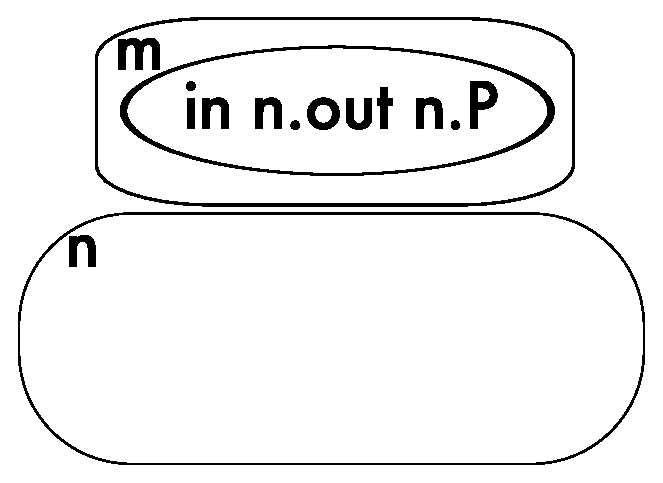
\includegraphics[scale=0.3]{ambient1}
  \caption{Spatial diagram of $m[\ambin{n}.\ambout{n}.P] \mid n[]$}
  \label{fig:ambient1}
\end{figure}

\begin{figure}  
  \centering
  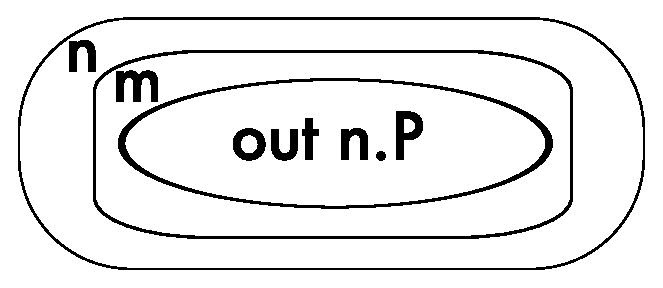
\includegraphics[scale=0.3]{ambient2}
  \caption{Spatial diagram of $n[m[\ambout{n}.P]]$}
  \label{fig:ambient2}
\end{figure}

\begin{figure}  
  \centering
  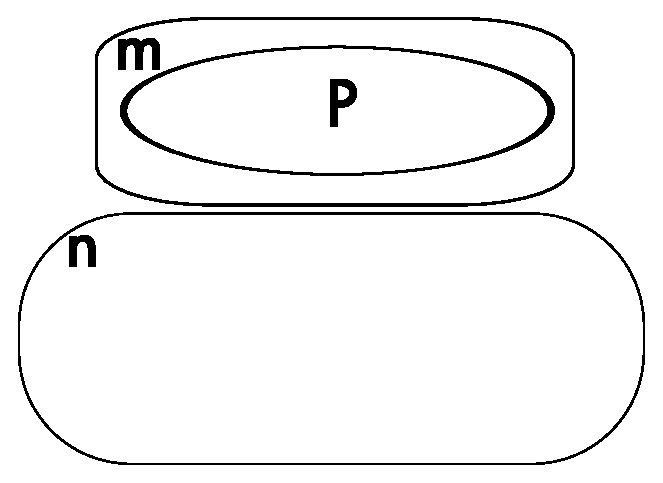
\includegraphics[scale=0.3]{ambient3}
  \caption{Spatial diagram of $m[P] \mid n[]$}
  \label{fig:ambient3}
\end{figure}

$open\ n$ is quite different.  It alters the structure, just as $in$ and
$out$ do, but rather than moving ambients, it destroys them.  It is also
applied to a child ambient rather than to the surrounding ambient, so
$open\ m.P\ |\ m[Q]$ (as in \cite{amb}) reduces to $P\ |\ Q$.

There are also issues with regard to the applicability of capabilities
and the use of the names.  A capability may only cause movement to occur
when at least one applicable ambient is available.  As such, movement
is heavily dependent on context, and specifically the availability of an
appropriately named ambient.  Applicability is dependent upon the
capability involved:

\begin{itemize}
\item For $\ambin{m}$, there must be a sibling of the surrounding
ambient named $m$.
\item For $\ambout{m}$, the parent of the surrounding ambient must be
named $m$.
\item For $\ambopen{m}$, there must be a child of the surrounding
  ambient named $m$.
\end{itemize}

All three capabilities are non-deterministic.  The same ambient name may
occur more than once, and each occurrence is regarded as being distinct.
As a result, the reduction of a capability includes a choice if there is
more than one applicable ambient present.  For example, $open\ m.P\ |\
m[Q]\ |\ m[R]$ has two possible derivations,

\begin{enumerate}
\item $open\ m.P\ |\ m[Q]\ |\ m[R] \rightarrow P\ |\ Q\ |\ m[R]$
\item $open\ m.P\ |\ m[Q]\ |\ m[R] \rightarrow P\ |\ m[Q]\ |\ R$
\end{enumerate}

The issue of non-determinism illustrates the behaviour that occurs when
there is more than one applicable ambient.  What about when there are
none?  The process stalls, and can not move on until such an ambient
becomes available.  This is akin to the situation in channel-based
calculi, such as CCS or the $\pi$ calculus, where a name is restricted,
but the appropriate co-name is not available to provide synchronisation.
For example,

\begin{equation}
(a.P) \backslash a 
\end{equation}

\noindent may never progress to become $P$ as there is no $\overline{a}$
for $a$ to synchronize with.  This behaviour is particularly relevant
with respect to $\ambout{m}$, where the sole use of the name is to stop
the surrounding ambient leaving its parent if the names don't match.

The restriction of ambient names, via $(\nu n) E$, combined with
mobility means that scope extrusion is also present in the calculus.
Just as the transmission of a name outside its scope causes extrusion
in the $\pi$ calculus, the restriction of ambient names may float
outward as necessary.  Scope intrusion is also possible in both
calculi, as demonstrated by the presence of the structural congruence
rule,

\begin{equation}
(\nu n)(P \pc Q) \equiv P \pc (\nu n) Q\ \text{if}\ n \not \in fn(P) \tag{Struct Res Par}
\end{equation}

\noindent which allows the restriction of $n$ to be removed from $P$
if the name doesn't occur free within its body.

\subsection{Variants of the Ambient Calculus}
\label{ambvariants}

A general problem within concurrency is the possibility of
\emph{interference}.  This was touched on briefly in the introduction
to this review, where the value of $x$ differed due to a race
condition.  In the ambient calculus, \emph{redex interference}
\cite{sangiorgi:mobsafeambients} is an issue, and is related to the
non-determinism mentioned above.

Take the example process from \cite{sangiorgi:mobsafeambients}.

\begin{equation}
n[\ambin{m}.P] \pc m[Q] \pc m[R]
\end{equation}

\noindent It is unclear what the environment of $P$ will be, following
the reduction of the capability, $\ambin{m}$.  There are two
alternatives,

\begin{enumerate}
\item $n[\ambin{m}.P] \pc m[Q] \pc m[R] \rightarrow m[n[P] \pc Q] \pc m[R]$
\item $n[\ambin{m}.P] \pc m[Q] \pc m[R] \rightarrow m[Q] \pc m[n[P] \pc [R]]$
\end{enumerate}

\noindent resulting from the two redexes formed between
$n[\ambin{m}.P]$ and $m[Q]$, and $n[\ambin{m}.P]$ and $m[R]$.  If one
contracts, resulting in a reduction, the other is no longer possible.
However, in this case, all three processes, $P$, $Q$ and $R$, can
still interact following either reduction.

In another example from the same paper,

\begin{equation}
\ambopen{n}.P \pc \ambopen{n}.Q \pc n[R]
\end{equation}

\noindent again with two possible interactions

\begin{enumerate}
\item $\ambopen{n}.P \pc \ambopen{n}.Q \pc n[R] \rightarrow P \pc \ambopen{n}.Q \pc R$
\item $\ambopen{n}.P \pc \ambopen{n}.Q \pc n[R] \rightarrow
  \ambopen{n}.P \pc Q \pc R$
\end{enumerate}


\noindent the resulting process includes a process, either $\ambopen{n}.Q$
or $\ambopen{n}.P$, which is stuck until such a time as another ambient
named $n$ appears as a child.  This may never occur.  These kinds of
interference, referred to in \cite{sangiorgi:mobsafeambients} as
\emph{plain interferences}, may occur in other calculi.  The equivalent
in the $\pi$ calculus would be:

\begin{equation}
\overline{x}z.P \pc x(y).Q \pc x(y).R
\end{equation}

\noindent where again a reduction will occur between one of the two:

\begin{enumerate}
\item $\overline{x}z.P \pc x(y).Q \pc x(y).R \rightarrow P \pc Q\{z/y\}
  \pc x(y).R$
\item $\overline{x}z.P \pc x(y).Q \pc x(y).R \rightarrow P \pc x(y).Q
  \pc R\{z/y\}$
\end{enumerate}

\noindent and the remaining process, either $x(y).Q$ or $x(y).R$, will
be blocked.

Another more serious form of interference may occur in the ambient
calculus, due to the provision of differing interactions ($\ambin{m},
\ambout{m}$ and $\ambopen{m}$).  These \emph{grave interferences} occur
when an ambient is involved in two reductions occurring as the result
of different types of capability.  Take the example process,

\begin{equation}
\ambopen{n}.\nil \pc n[\ambin{m}.P] \pc m[Q]
\end{equation}

\noindent in which two reductions can occur that are logically
different.  While the interferences described above are a
representation of the kind of race conditions and non-determinism that
would be expected in any concurrent model, for example, to represent
competition for resources, grave interferences are usually unexpected
and typically represent errors in the model.  This process may perform
two radically different reductions,

\begin{enumerate}
\item $\ambopen{n}.\nil \pc n[\ambin{m}.P] \pc m[Q] \rightarrow \nil \pc
\ambin{m}.P \pc m[Q]$
\item $\ambopen{n}.\nil \pc n[\ambin{m}.P] \pc m[Q] \rightarrow
\ambopen{n}.\nil \pc m[n[P] \pc Q]$
\end{enumerate}

\noindent where either $n$ is destroyed, thus preventing the latter
movement of $P$ in to $m$ as it has no surrounding ambient, or $n$ moves
inside $m$ and is no longer available to be destroyed by
$\ambopen{n}.\nil$.  Clearly, only one of these reductions is likely to be
intentional.  

Levi and Sangiorgi's calculus of Mobile Safe Ambients
\cite{safeamb00,sangiorgi:mobsafeambients} presents a solution to
this.  It introduces a notion of co-capabilities, which enforce a
pairing of mobility primitives before a reduction can be made.  The
result of this is that the ambient being entered, exited or opened is
aware of what is taking place, and may react accordingly.

With these co-capabilities in place, the reduction rules for the
calculus run as follows:

\begin{align}
 n[\ambin{m}.P_1 \pc P_2] \pc m[\sambin{m}.Q_1 \pc Q2]
\rightarrow
m[n[P_1 \pc P_2] \pc Q_1 \pc Q_2] \tag{SafeIn}\\
 m[n[\ambout{m}.P_1 \pc P_2] \pc \sambout{m}.Q_2 \pc Q2]
\rightarrow
n[P_1 \pc P_2] \pc m[Q_1 \pc Q_2] \tag{SafeOut}\\
 \ambopen{n}.P \pc n[\sambopen{n}.Q_1 \pc Q_2]
\rightarrow
P \pc Q_1 \pc Q_2 \tag{SafeOpen} 
\end{align}

\noindent where, in each case, the capability must be able to
synchronize with a co-capability in the relevant ambient for the
reduction to take place.  For example, in SafeIn, $\ambin{m}.P_1$ must
pair up with $\sambin{m}.Q_1$ in the ambient $m$.  As a result, $Q_1$
can react appropriately to the change in structure, based on the fact
that it knows the movement has occurred.

The changes in the calculus of safe ambients, though simple, have a
dramatic effect on the ability to construct an algebraic theory for
the calculus and prove properties, especially when coupled with an
appropriate type system\footnote{In this case, the type system ensures
  single-threadedness, where only one process within an ambient may
  exercise a capability.}.  Essentially, they represent a move from
asynchronous to synchronous mobility primitives.  The calculus of
controlled ambients \cite{controlledamb02} restricts behaviour
further, by requiring that a co-capability must appear in both the
source and the destination.  Thus, an $\ambin{m}$ capability requires
permission both to leave its current location and to enter the
destination ambient. This is useful for the specific application of
the calculus, controlling resources, but is excessive in most
circumstances.

A further variant of the ambient calculus is the calculus of boxed
ambients \cite{boxedamb01}.  This removes the $open$ capability
altogether, replacing it with a form of directed communication inspired
by \cite{seal}.  Processes remain within their initial ambient
permanently (hence the term `boxed') and only the structure of the
ambient topology changes via the $in$ and $out$ capabilities.  Messages
may be sent locally, upwards or downwards, but not to siblings.

An example process from \cite{boxedamb01} is:

\begin{equation}
n[(x)^pP \pc p[\langle M \rangle \pc (x)Q \pc q[\langle N
\rangle^\uparrow ]]]
\end{equation}

\noindent where $n$, $p$ and $q$ are ambients, both $(x)$s are inputs
and $\langle M \rangle$ and $\langle N \rangle$ represent outputs.
The use of the superscript on $(x)^p$ indicates a downward
communication into the ambient $p$, while the use of $\uparrow$ in
$\langle N \rangle^\uparrow$ indicates an upward communication
directed at the parent ambient.  Thus, $(x)Q$ may synchronize with
either $\langle M \rangle$ locally or the upward communication from
$\langle N \rangle$.  $(x)^pP$ must synchronize with $\langle M
\rangle$, as the only output in $p$.

The ideas behind the boxed ambients calculus result in a formalism which
is more suited to communication-focused modelling, where the destruction
of locations would be unnatural.  Both it and the original ambient
calculus have their own particular niche, being suited to particular
applications.  In contrast, the latter is clearly more suited to
situations where the removal of a locality corresponds to a similar
event in the real-world situation being modelled.

\subsection{Advantages and Disadvantages of the Ambient Calculus}

The most interesting aspect of the ambient calculus is that, while it
includes no communication primitives, it can encode the asynchronous
$\pi$ calculus (see \ref{pivariants}).  This seems to imply that it is
possible to model mobility in a more natural way without losing much of
the expressivity of the $\pi$ calculus.  On consideration , this seems a
little less surprising as ambient names exhibit the same scope extrusion
seen with channel names in the $\pi$ calculus.  With this in mind, it is
not too difficult to see that ambient names could be used to mimic
channel names, with synchronisation being emulated by two processes
performing some kind of interaction within the same ambient.

However, the representation of synchronisation illustrated in \cite{amb}
seems to suggest that the ambient calculus may still have problems
dealing with the kind of global synchronisation needed for the
compositional broadcast agent considered in \ref{ccslimit}.  The
operation is performed by destroying and recreating ambients, as a
signal to the other process involved in the synchronisation.  Extending
this would seem to require using more ambients, which again leads to the
problem of enumerating the number of entities who wish to synchronize.
As before, this is possible but not compositional; every time
synchronisation is performed with a different number of agents, the
semantics of the process must be recreated.

Thus, the ambient calculus and the $\pi$ calculus have more in common
than is initially apparent, and the choice between the two seems to be
largely based on the most natural formalism for a particular task.

%\subsubsection{The Seal Calculus}

%The seal calculus \cite{seal}

\subsection{P Systems}
\label{psystems}

While providing a way of modelling concurrent spatially-oriented
systems, P Systems \cite{membranecomp,membranehandbook} arise from
the area of formal language theory and re-writing rules rather than
process calculi.  They are considered here, as there exist a number of
similarities between them and, for example, the ambient calculus both
in providing a distributed model of computation and in finding
applications in the area of biological modelling.  Below, a basic P
system with priorities is introduced.

A transition P system with priorities \cite{paun:98membranes} of
degree $n$, where $n \ge 1$ is represented as:

\begin{equation}
\Pi = (V, \mu, M_1, \dots, M_n,(R_1,\rho_1), \dots, (R_n,\rho_n),i_0)
\end{equation}

\noindent where:

\begin{itemize}
\item $V$ is an alphabet of objects.
\item $\mu$ is the membrane structure, containing $n$ membranes.
\item $M_i$, where $1 \le i \le n$, is a multiset of objects from $V$
      which are contained in membrane $i$.
\item $R_i$, where $1 \le i \le n$ is an evolution rule associated
  with one of the membranes, $i$. The corresponding $\rho_i$ is a
  partial-order relation which determines the priority of the rule.
  The rules are rewriting rules of the form $a \rightarrow v$, which
  causes $a$ to be replaced by $v$; where $a \in V$ and $v \in (V
  \times Tar)^*$, $Tar = \{here, out, in | 1 \le i \le n\}$.  The set
  $Tar$ of target regions gives all the possible derivations for
  symbols occurring on the right-hand side of each rule.  Rules of the
  form $a \rightarrow v\delta$ indicate the membrane will disappear
  after its application.
\item $i_0$ is a number between 1 and $n$ which specifies the
  \emph{output membrane} where the result of the computation should be
  found.
\end{itemize}

\noindent Any of the multisets, rules or priority relations may be
empty.  Evolution occurs in parallel, in a synchronous fashion
involving all membranes (referred to as \emph{maximal parallelism}).
A universal clock is assumed to exist, which breaks the evolution of
the system into cycles.  Objects may move between membranes and
membranes may be broken, causing their objects to flood into the
membrane above and their rules to disappear.  Such behaviour has
echoes of the ambient calculus described in \ref{ambientcalculus},
where ambients may be destroyed by the $open$ primitive and processes
may move around the ambient hierarchy (but only within an ambient).
The notion of synchronous clock cycles also recalls the discrete timed
calculi of chapter \ref{globsync}, where evolution can also be bounded
by clock cycles in a synchronous fashion.  An interesting distinction
is commonly made in P systems; the outer membrane or \emph{skin
  membrane} is assumed to be special.  For example, at least in a
biological context, the system is assumed to terminate if the outer
membrane is destroyed (biologically, the external membrane has been
broken and thus the organism falls apart).

Consider the following example P system (Fig. \ref{fig:psystem}),
\begin{align*}
\Pi_1 & = (V, \mu, M_1, M_2, M_3, M_4, (R_1, \rho_1), (R_2, \rho_2),
 (R_3, \rho_3), (R_4, \rho_4),4) \\
V & = \{a,b,b',c,f\} \\
\mu & = [_1[_2[_3]_3[_4]_4]_2]_1 \\
M_1 & = \emptyset, 
R_1 = \emptyset,
\rho_1 = \emptyset \\
M_2 & = \emptyset, 
R_2 = \{b' \rightarrow b, b \rightarrow b(c, in_4), r_1 : ff
 \rightarrow af, r_2 : f \rightarrow a\delta\},
\rho_2 = \{r_1 > r_2\} \\
M_3 & = \{af\},
R_3 = \{a \rightarrow ab', a \rightarrow b'\delta, f \rightarrow ff\},
\rho_3 = \emptyset \\
M_4 & = \emptyset,
R_4 = \emptyset,
\rho_4 = \emptyset
\end{align*}

\begin{figure}  
  \centering
  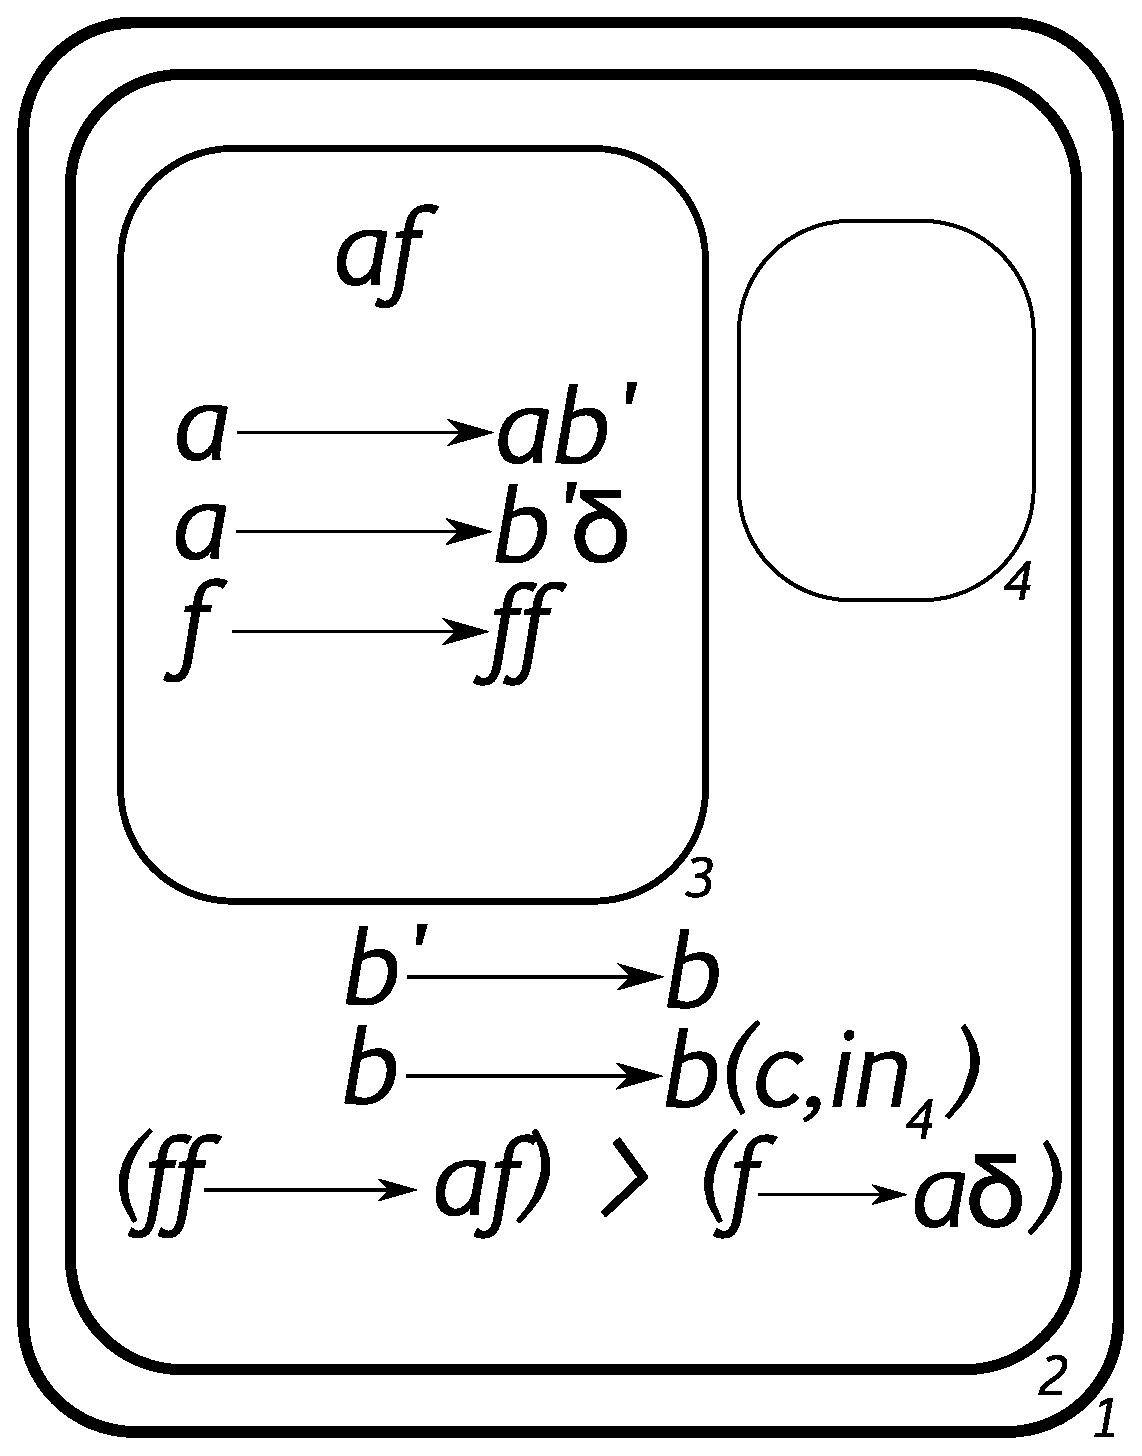
\includegraphics[scale=0.3]{psystem}
  \caption{Example P System}
  \label{fig:psystem}
\end{figure}

\noindent where the only membrane that initially contains any objects is
$M_3$.  In $M_3$ are two objects, $a$ and $f$.  $f$ only matches one
rule, $f \rightarrow ff$, which causes the number of $f$s to double on
each evolution.  For $a$, there are two rules and one is chosen
non-deterministically.  If the first, $a \rightarrow ab'$, is applied,
then an additional object $b'$ appears, and the rule may be applied
again as an $a$ is still present.  If $a \rightarrow ab'$ and $f
\rightarrow ff$ are applied for $n$ steps, then $n$ instances of $b'$
and $2^n$ occurrences of $f$ are present.

If the second $a$ rule $a \rightarrow b'\delta$, is applied, the
$\delta$ causes the membrane, $M_3$, to be dissolved.  At this point,
there will be one extra $b'$ and one extra $f$ resulting from the
application of this rule and $f \rightarrow ff$, respectively, and no
$a$.  This changes the configuration of the system to become:
\begin{align*}
\mu & = [_1[_2[_4]_4]_2]_1 \\
M_1 & = \emptyset, 
R_1 = \emptyset,
\rho_1 = \emptyset \\
M_2 & = \{b'^{n+1}, f^{2n+1}\} \\ 
R_2 & = \{b' \rightarrow b, b \rightarrow b(c, in_4), r_1 : ff
 \rightarrow af, r_2 : f \rightarrow a\delta\},
\rho_2 = \{r_1 > r_2\} \\
M_4 & = \emptyset,
R_4 = \emptyset,
\rho_4 = \emptyset
\end{align*}

\noindent The three rules that were present in $M_3$ are lost, while the
objects float into the membrane above, $M_2$.  In this configuration,
$n$ represents the number of times the pair of rules $a \rightarrow ab'$
and $f \rightarrow ff$ were applied prior to this, and is greater than
or equal to zero.

In $M_2$, a priority relation exists that forces $ff \rightarrow af$ to
be given precedence over $f \rightarrow a\delta$.  As a result, whenever
it is possible to apply $ff \rightarrow af$ (i.e. there are two $f$
objects), it will be applied instead of $f \rightarrow a\delta$.  The
other two rules manipulate the $b'$ objects. First, they are all
converted in to $b$ objects.  This will always occur, as there are at
least two $f$ objects in $M_2$ to begin with, which means $ff
\rightarrow af$ will be applied rather than $f \rightarrow a\delta$
which destroys $M_2$.  Each time $ff \rightarrow af$ is applied, the
number of $f$ objects halves.

The remaining rule, $b \rightarrow b(c, in_4)$, will evolve once for
each occurrence of $ff$, of which there are $n$.  $M_2$ contains $n + 1$
$b$ objects, all converted from the $b'$ objects that were in $M_3$.  As
long as there is an even number of $f$ objects, the two rules $b
\rightarrow b(c, in_4)$ and $ff \rightarrow af$ will be applied, halving
the number of $f$ objects and creating $n + 1$ c objects in $M_4$ (via
$(c, in_4)$), while the number of $b$ objects remains the same.

When only one $f$ object is left, $f \rightarrow a\delta$ will be
applied, resulting in $M_2$ being destroyed and the following
configuration:
\begin{align*}
\mu & = [_1[_4]_4]_1 \\
M_1 & = \{a^{2n+1},b^{n+1}\}, 
R_1 = \emptyset,
\rho_1 = \emptyset \\
M_4 & = \{c^{(n+1)^2}\},
R_4 = \emptyset,
\rho_4 = \emptyset
\end{align*}

\noindent No further evolution is possible, as there are no more rules.
$c^{(n+1)^2}$ is the final output, as $M_4$ is the output membrane.

Further variants of P systems exist.  Tissue P systems use a
graph-based structure rather than the tree shown here, while
population P systems also incorporate an environment and use a dynamic
graph as an associated structure of it.  There are also timed variants
of P systems; rules are usually assumed to apply instantaneously, but
in the timed variants they can take a specific duration.

\section{Comparing Modelling Approaches}
\label{bioapps}

Biological systems are inherently concurrent, being focused on the
behaviour of multiple entities from low-level molecules, through
bacteria and other bodies, to full cellular structures and beyond.
Models which incorporate spatial distribution, such as the ambient
calculus (\ref{ambientcalculus}) and P systems (\ref{psystems}) are
especially useful for representing the structure of real-world
biological entities.

Such modelling is becoming commonplace within the literature
 \cite{fran,cardelli:bioambients,biospi}, where concurrent models
represent an alternative to the use of ordinary differential equations
(ODEs).  The usual approach is to create a model of the system within
the formalism and then perform simulations.  Such simulations rely on
reducing the non-determinism within the model by introducing a
stochastic semantics.  In each of the biochemical stochastic $\pi$
calculus \cite{biospi}, the BioAmbient variant
\cite{cardelli:bioambients} and P systems \cite{fran}, these are based
on Gillespie's algorithm \cite{gillespie}.

The algorithm selects which reaction occurs next and the necessary
advancement of the system's `clock' (a real time value in this context,
rather than some discrete notion).  A probability is associated with
each reaction, so that the algorithm basically runs as follows:

\begin{enumerate}
\item $a_0$ is calculated as the sum of the probabilities.
\item Two random numbers, $r_1$ and $r_2$, are generated from a uniform
      distribution over the unit interval 0 to 1.
\item Calculate the waiting time for the next reaction, $\tau_i =
      \frac{1}{a_0} \ln (\frac{1}{r_1})$
\item Take the index, $j$, of the reaction such that
      $\displaystyle\sum_{k=1}^{j-1} p_k < r_2 a_0 \le
      \displaystyle\sum_{k=1}^jp_k$ where $p_k$ is the $k$th probability.
\item Return the pair $(\tau_i, j)$
\end{enumerate}

\noindent determining which one occurs.  Slight alterations are made in
distributed models to handle the rules arising from different localities.
For example, the P systems model \cite{fran} adapts the algorithm to
form a multi-compartmental variant, which treats each membrane
separately, to a degree, while also taking into account that activity
in one membrane may affect others.

Clearly, different formalisms offer different approaches.  In the
original $\pi$ calculus approach of \cite{biospi}, the focus was solely
on communication with biological compartments abstracted as private
channels.  The model given for BioAmbients \cite{cardelli:bioambients}
is more natural due to the explicit realisation of these compartments.

Take the following example from \cite{cardelli:bioambients},

\begin{equation}
\begin{aligned}
\mathtt{System} & ::= \mathtt{molecule[Mol] \pc \dots \pc molecule[Mol] \pc
 cell[Porin]} \\
\mathtt{Mol} & ::= \mathtt{enter\ cell1.Mol + exit\ cell2 . Mol} \\
\mathtt{Porin} & ::= \mathtt{accept\ cell1.Porin + expel\ cell2.Porin}
\end{aligned}
\end{equation}

\noindent which demonstrates a membranal pore, which molecules use to
pass through a membrane.  Both the cell and the molecules are
represented by ambients.  Each molecule is controlled by a process,
$Mol$, which, at any time, has the option of performing either an
\texttt{enter} or an \texttt{exit}.  Similarly, the $Porin$ process,
which represents the membranal pore, may \texttt{accept} or
\texttt{expel}.

Within the BioAmbient calculus, movement is synchronous and takes place
by the pairing of an \texttt{enter} and \texttt{accept} action (the
equivalent of $in$) or an \texttt{exit} and \texttt{expel} action
(equivalent to $out$).  The first action in each case is used by the
moving process.  Both must also mention the same channel name
(\texttt{cell1} and \texttt{cell2} here).  In the case of the system
shown above, both \texttt{Mol} and \texttt{Porin} permanently offer
their halves of this pairing.  However, the spatial context makes one of
them inapplicable.  Initially, \texttt{exit} and \texttt{expel} won't
synchronize, as \texttt{Mol} is not inside the ambient from which it is
being expelled.  Likewise, once it has entered, it can't do so again,
even though the actions make this possible.

Models such as this seem a little unnatural as molecules are modelled as
both an ambient and a process.  This is because only ambients may move
but only processes can emit the necessary mobility primitives to do so.
The notions of mobility present in the ambient calculus, including this
idea, have been carried across, even though it doesn't directly adopt
the primitives of the ambient calculus; the style is still more akin to
the $\pi$ calculus.

In contrast, \cite{fran} takes a different approach using P systems,
representing signals and proteins directly as objects in the membranes.
One particular application of this technique is \emph{quorum sensing}.
This is a gene regulation system where a population of bacterial cells
communicate in order to regulate the expression of certain genes in a
co-ordinated way which is dependent on the size of the population.
\cite{fran} presents a model of this phenomenon in \emph{vibrio
fischeri}, a marine bacterium, using a P system\footnote{This method of
defining the configuration differs slightly from that in \ref{psystems},
as it also includes a set of labels, rather than assuming that the
natural numbers are used.}:
\begin{align*}
  \Pi_{vf} & = (O, \{e,b\}, \mu, (w_1, e), (w_2, b), \dots,
  (w_{n+1},b),\mathcal{R}_b, \mathcal{R}_e) \\
  O & = \{\OHHL, \LuxR, \LuxR\text{-}\OHHL, \LuxBox, \LuxBox\text{-}\LuxR\text{-}\OHHL\} \\
  w_1 & = \emptyset \\
  w_i & = \{\LuxBox\}\ \text{where}\ 2 \le i \le n + 1 \\
\end{align*}

\noindent where each bacteria is represented as a membrane, $b$, within
an environment membrane, $e$.  The alphabet, $O$, contains the signal,
$\OHHL$, the protein, $\LuxR$ and the regulatory region, $\LuxBox$, in
addition to the protein-signal complex ($\LuxR$-$\OHHL$) formed and its
regulatory region, $\LuxBox$-$\LuxR$-$\OHHL$.  The initial configuration shown
above leaves the environment empty and places just the genome, $\LuxBox$,
inside each bacteria membrane to start production of the signal and the
protein.  $\mathcal{R}_b$ and $\mathcal{R}_e$ contain the rules which
affect the bacteria and the environment respectively.  The reader is
referred to the full paper for full details of these.

There are similarities between process calculi and P systems, even
though they arose from two different communities.  Many of the same
techniques and properties have been proven to apply to both, and it is
possible to translate a P system into a process calculus form to take
advantage of model checking techniques originally designed for a
process calculus.  The difference in their backgrounds also results in
some interesting differences in their design and the way they are
used; P systems arise from language generation and thus the rules are
applied in parallel, while on the other hand, process calculi are
usually based around transitions and communication.  The choice of
which one is best to use really depends upon the use to which it is
being put; P systems make sense when there is structure inherent in
the model and the various process algebraic techniques lend themselves
to situations with a large amount of communication that needs to be
monitored.

\section{Bigraphs}
\label{bigraphs}

Bigraphs \cite{bigraph1,bigraph2} are an attempt at providing a
unifying framework, able to represent both spatial relationships
(\emph{locality}) in the style of the ambient calculus (see
\ref{ambientcalculus}) and link-based-relationships
(\emph{connectivity}) seen in the $\pi$ calculus (see \ref{picalculus}).
Their particular application area is within pervasive computing, where a
mixture of both concepts is needed to represent both movement through
space and the change in relationships between agents.

The nodes in a bigraph support a dual structure, hence the name.  On one
level, there are nodes nested within nodes, representing locality.  This
is called the \emph{place graph}.  These nodes have \emph{ports} which
are connected via links to form a \emph{link graph}.  Each node has a
\emph{control} with an arity that defines the number of ports.  The two
graphs share nodes, but are otherwise independent.  Nesting can only
occur in nodes with a \emph{non-atomic} control.  These can also be
\emph{active} or \emph{passive}.  The former allows reactions to occur
within the node.  \emph{Holes} may occur in bigraphs, where other
bigraphs can appear.

Within this model, it is possible to encode both the $\pi$ calculus and
the ambient calculus.  Take the following rule from the asynchronous
$\pi$ calculus without summation,

\begin{equation}
\overline{x}y \pc x(z).P \rightarrow P\{y/z\}
\end{equation}

\noindent which represents synchronisation.  In \cite{bigraph1}, Milner
encodes this as a bigraph with two controls, $send$ and $get$, both of
which have an arity of two.  To represent the fact that the output
prefix has no continuation in the asynchronous $\pi$ calculus, $send$ is
declared atomic.  $get$ is non-atomic but inactive.

The node $get$ includes a nested hole with the port $z$.  This
represents the continuation $P$, with $z$ being the name bound on
input.  The port $z$ is linked from the hole to $get$ itself.  $send$
has two ports: $x$, which is also connected to $get$, and $y$.  With
these concepts in place, the reaction may be represented as:

\begin{equation}
send_{xy} \pc get_{x(z)} \square \rightarrow x \pc y/(z) \square
\end{equation}

\noindent the $send$ node disappearing afterwards, leaving $y$ connected
to $z$ and $x$ unused.

Similarly, \cite{bigraph1} shows how the $in$ capability from the
ambient calculus:

\begin{equation}
 n[\ambin{m}.P_1 \pc P_2] \pc m[Q]
  \rightarrow
  m[n[P_1 \pc P_2] \pc Q] \\
\end{equation}

\noindent may be encoded using two controls, $amb$ and $in$, both with
an arity of one.  The two ambients involved are represented by
instances of $amb$, while $in$ is an atomic control representing the
process that emits the capability.  The $amb$ control is non-atomic
and active, each ambient containing a hole which represents their
continued behaviour,

The ambient names are represented as the node's single port.  In the
case of the ambient named in the capability, this is also linked to the
$in$ instance.  To model the reaction above, $n$ is connected to the
port of one $amb$, while $m$ is connected to both the other $amb$ and
$in$.  The reaction is then encoded as:

\begin{equation}
amb_n (in_m \pc \square_0) \pc amb_m \square_1
\rightarrow
amb_m (amb_n \square_0 \pc \square_1)
\end{equation}

\noindent where the similarities between the two are clear.

Bigraphs provide an interesting framework for unifying the two
disparate concepts outlined above in \ref{scopemobility} and
\ref{migration}.  It will be exciting to see how this theory develops,
and whether it can also be used to encode the discrete time notions
described in chapter \ref{globsync}.

\section{Conclusion}

The $\pi$ calculus seems to provide the best of both worlds, being able
to model concurrent systems and still retain the expressiveness of the
$\lambda$ calculus.  However, a key limitation was identified which
reinforced the idea that expressivity only makes a model capable, and
not suitable, for simulating any recursive function: modelling global
synchronisation via a broadcasting agent.  This limitation seems to hold
for both CCS and the $\pi$ calculus, and it is also likely that it
applies to many other process calculi, such as the ambient calculus, a
formalism that provides a more natural form of mobility via structural
changes.

Biology was also considered briefly (see \ref{bioapps}), as a
motivating paradigm.  P systems seem the most natural formalism in
this area and there are clear parallels between P systems and ambient
calculi, especially in their use of structure.  In the next chapter,
we take the general concepts of structural change and migrating
objects present in both, and combine them with CaSE to create a new
calculus; Nomadic Time.


% Our Process Calculus
% Thesis: Nomadic Time
% Author: Andrew Hughes

\chapter{Nomadic Time}
\label{nt}

\section{Introduction}

This chapter introduces the process calculus used as the basis for
DynamiTE, Nomadic Time, in which timed processes are mobile.  Over the
course of the first half of this chapter, we show how CaSE \cite{CaSE}
(itself a timed derivative of CCS) is first extended with localities
(see \ref{localising}) and then mobility (see \ref{addingmob}) to
create a calculus which provides both the ability to migrate processes
during execution and to perform global synchronisation in a
compositional manner.  We then introduce the concept of `bouncers'
(see \ref{bouncers}), which allow migration to be restricted; they
define which mobility actions may be performed and how many times.
This is followed by the operational semantics of the calculus (see
\ref{ntsemantics}).  Finally, we close with a comprehensive example
(see \ref{example}) demonstrating each feature of the calculus and the
application of the calculus to our prototypical application (see
\ref{app:nt}).

\section{Localising the Calculus}
\label{localising}

\emph{Localisation}, discussed in detail in \ref{migration}, effectively
adds another level of grouping to the calculus.  A set of composed
processes may be contained within one \emph{locality}, a notion which is
often used in the modelling of \emph{distribution}.  This idea, which
can be taken to its logical conclusion by forming a hierarchy of such
localities, has echoes of the notion of \emph{clock hiding} within CaSE,
as described in \ref{case}.

Thus, the first step in the evolution towards NT is to combine these
two hierarchical concepts by effectively localising CaSE.  The notion of
components and encapsulation is explicitly realised by an
\emph{environ}, which also handles the hiding of clocks.  As a result,
the clock hiding operator from CaSE disappears, being replaced by a new
operator which allows the creation of environs.  The bounds of the
environ define both a new group and the scope of the clock hiding.  The
syntax for localised CaSE is thus:
\begin{equation}
  \begin{aligned}
    \expr, \exprb\ ::=\ &
    \nil  \;\,|\,\; 
    \Delta \;\,|\,\; 
    \Delta_{\sigma} \;\,|\,\; 
    \alpha . \expr  \;\,|\,\;
    \expr + \exprb \;\,|\,\; 
    (\expr\;|\;\exprb)\;\,|\,\; 
    \timeout{\expr}{\sigma}{\exprb} \;\,|\,\; \\
    & \stimeout{\expr}{\sigma}{\exprb} \;\,|\,\; 
    \mu X . \expr \;\,|\,\; 
    X \;\,|\,\; 
    \expr \setminus a \;\,|\,\; 
    \lclocv{m}{\expr}{\vec{\sigma}}
  \end{aligned}
\end{equation}
where $\vec{\sigma}$ is a set of clocks and $m$ represents an
arbitrary environ name\footnote{Note that although names are added to
  the environs here, this is not really necessary at this stage; they
  provide nothing more than a way to refer to environs in talking
  about a system.  However, they are necessary for providing migration
  as discussed in \ref{migration}}.  In particular, $m$ may be equal
to the empty string, $\epsilon$, thus facilitating the use of
anonymous environs.  This allows the semantics of CaSE's clock hiding
to be encoded:

\begin{equation}
\seml E / \sigma \semr \eqdef \lcloc{}{E}{\sigma}
\end{equation}

\noindent thus making localised CaSE a conservative extension.  The
environs form a forest structure, due to the ability to nest
environs to an arbitrary depth and the possibility of multiple
environs occurring at the top level.

Recall the example of clock hiding given in (\ref{clockhidingex}):
\begin{equation}
  (P / \sigma)\;|\;Q
\end{equation}
This becomes:
\begin{equation}
  \lcloc{}{P}{\sigma}\;|\;Q
\end{equation}
in localised CaSE, or:
\begin{equation}
  \lcloc{m}{P}{\sigma}\;|\;Q
\end{equation}
if an arbitrary name, $m$, is assigned to the environ.  Just
as with the clock hiding operator, the clock $\sigma$ is hidden outside
the environ, $m$, causing its ticks to be visible only to $P$.  

With this extension the set of visible clocks for a particular environ
may be obtained by finding the set difference between $\timers$ and
the union of the sets of clocks of its child environs.  For example,
consider the more complex scenario:
\begin{equation}
\lcloc{n}{E\;|\;\lcloc{m}{F\;|\;\lcloc{k}{G}{\sigma}}{\rho}}{\gamma}
\end{equation}
where the top-level environ, $n$, contains a process $E$ and a further
sub-environ, $m$.  Likewise, $m$ contains both a process, $F$, and the
sub-environ, $k$.  Finally, $k$ contains just the single process, $G$.
The set of clocks for the environ $k$ is $\{\sigma\}$ and its parents
are $m$ (with the set $\{\rho\}$) and $n$ (with $\{\gamma\}$).  Thus,
the set of visible clocks for $k$ is $\timers \backslash \emptyset$,
as it has no child environs.  which means that $G$, located in $k$,
can see the ticks of all clocks.

$F$, by comparison, can only see the ticks of the clocks in $\timers
\backslash \{\sigma\}$ as $\sigma$ is hidden outside $k$.  $E$, in the
top-level environ, $n$, can only observe silent actions resulting from
the two hidden clocks, $\rho$ and $\sigma$, but can see the ticks of
$\gamma$ and any other clocks in $\timers$, its set of visible clocks
being $\timers \backslash \{\sigma, \rho\}$.

\section{Adding Mobility}
\label{addingmob}

Localised CaSE makes the notion of components and encapsulation clearer
than in the original calculus, by allowing them to be given explicit
names.  However, it doesn't provide a great deal of extra
functionality\footnote{Although the semantics could be adapted so as to
use the environs for bisimulation, as in \ref{migration}.}.  The most
natural progression from this stage is to add mobility.  For this, the
primitives of the ambient calculus are adopted, as they provide a very
natural and simplistic formalism, which builds on the component-oriented
nature of the calculus, now explicitly realised by environs.  This is
shown in more detail in \ref{locmob}.

In addition, NT allows the movement of individual processes.  In the
ambient calculus, only ambients can move, which restricts the
separability of processes.  For a given group of processes, the
size of the group may only change by:

\begin{enumerate}
\item One of the processes becoming $\nil$.  Both NT and the ambient
      calculus include a structural congruence law,
\begin{equation}
E\;|\;\nil \equiv E
\end{equation}
      which allows such processes to be removed.
\item The process splitting into two or more processes via parallel
      composition.  For example, $\ambin{m}.(E | F)$ enters the ambient, $m$,
      and then splits into two separate processes, $E$ and $F$.
\item Another process \emph{open}ing the ambient, causing the set of
      processes to merge with those in the parent.
\end{enumerate}

What the ambient calculus doesn't allow is for a selected process or
group of processes to be moved from one ambient to another.  That
process or group must be in its own ambient for this to happen.

Take the example process, 
\begin{equation}
m[E\;|\;F\;|\;G]\;|\;n[\nil]\;|\;H
\end{equation}
where $E$, $F$, $G$ and $H$ are all processes and $m$ and $n$
are ambients.  The topology of this process may change in several ways, as
outlined above. Any of the four processes might evolve to $\nil$, or fork
into two or more processes.  In addition, $E$, $F$ or $G$ may emit an
$\ambin{n}$ capability, causing the ambient $m$ to move inside $n$.
Similarly, $H$ may perform an $\ambopen{m}$, causing $m$ to be removed and
the top-level to include all four processes.

So, several events may occur but there are also some that are intuitive,
but difficult to achieve.  For instance, all three processes in $m$ must
move as a unit, whether this is to the top-level due to an $open$
capability or as a result of $m$ moving in to $n$.  Moving one process,
$E$ for example, requires the interaction of both $E$ itself and another
process at the final destination.

To move $E$ to the top level on its own requires converting it to the
form,
\begin{equation}
Emov \eqdef z[\ambout{m}.E]
\end{equation}
where $z$ is a new name, which doesn't occur free in either
$E$, $F$, $G$ or $H$.  The effect is clearer when this is placed in
context,
\begin{equation}
m[z[\ambout{m}.E]\;|\;F\;|\;G]\;|\;n[\nil]\;|\;H
\end{equation}
where it can be clearly seen that the new capability prefixed
on $E$ will cause the new surrounding ambient, $z$, to move outside of
$m$.  To actually have $E$ at the top-level, and not $E$ nested in an
ambient, requires the presence of a top-level process to open the $z$
ambient.  This results in something along the lines of:
\begin{equation}
m[z[\ambout{m}.E]\;|\;F\;|\;G]\;|\;n[\nil]\;|\;H\;|\;\ambopen{z}.\nil
\end{equation}
to truly encode the movement of $E$ alone.  Moving just $E$
into $n$ is even more convoluted:
\begin{equation}
m[z[\ambout{m}.\ambin{n}.E]\;|\;F\;|\;G]\;|\;n[\ambopen{z}.\nil]\;|\;H
\end{equation}
and neither are particularly natural.  NT instead provides
this functionality as a base part of the syntax, which will be explored
in \ref{procmob}.  

Finally, it should be noted that the scope of an action is implicitly
restricted to the bounds of an environ within NT.  For instance, in the
following process:
\begin{equation}
a.P \pc \lcloc{m}{\overline{a}.Q}{\sigma}
\end{equation}
synchronisation between the two processes is not permitted as
they lie on either side of a environ boundary.  This is not an issue,
as the presence of mobility allows processes to move into a situation
where the co-action is in scope.  In addition, NT (at present) does not
incorporate the scoping of environ names.

\subsection{Location Mobility}
\label{locmob}

To add an ambient calculus style of mobility, the existing syntax of
localised CaSE is extended with a mobility prefix, $\ambop . \expr$,
to give:
\begin{equation}
  \begin{aligned}
    \expr, \exprb \mathrel{::=} &
    \nil  \;\,|\,\; 
    \Delta \;\,|\,\; 
    \Delta_{\sigma} \;\,|\,\; 
    \alpha . \expr  \;\,|\,\;
    \expr + \exprb \;\,|\,\; 
    (\expr\;|\;\exprb)\;\,|\,\; 
    \timeout{\expr}{\sigma}{\exprb} \;\,|\,\; \\
    & \stimeout{\expr}{\sigma}{\exprb} \;\,|\,\; 
    \mu X . \expr \;\,|\,\; 
    X \;\,|\,\; 
    \expr \setminus a \;\,|\,\; 
    \lcloc{m}{\expr}{\vec{\sigma}} \;\,|\,\;
    \ambop . \expr
  \end{aligned}
\end{equation}
where $\ambop$ is further defined as:
\begin{equation}
   \ambop \mathrel{::=} \tntin{m} \mid \tntout{m} \mid \tntopen{m} 
\end{equation}
with $m$ again representing the name of an environ.  The behaviour of
these primitives is identical to the behaviour of their equivalents in
the ambient calculus ($\tntin{m}$ being $\ambin{m}$, $\tntout{m}$ being
$\ambout{m}$ and $\tntopen{m}$ being $\ambopen{m}$)\footnote{The mnemonics
$\tntin{m}$, $\tntout{m}$ and $\tntopen{m}$ are used to prevent
confusion with the names of actions.}, so just a short recap of section
\ref{ambientcalculus} is given here, using the syntax above.  Note that
the syntactic abbreviation, $\lncloc{m}{E}$, is used to represent
$\lcloc{m}{E}{}$.

When a process emits an $\tntin{m}$ capability, the surrounding environ
may move into a sibling environ with the name, $m$.  Given the context,
\begin{equation}
\lncloc{m}{E}\;|\;\lncloc{n}{\nil}
\end{equation}
if $E$ is defined as
\begin{equation}
E \eqdef \tntin{n}.E^\prime
\end{equation}
then this will allow the derivation
\begin{equation}
\lncloc{m}{\tntin{n}.E^\prime \pc \lncloc{n}{\nil}} \derives{\tntin{n}} 
\lncloc{n}{\lncloc{m}{E^\prime} \pc \nil}
\end{equation}
to occur.  Similarly, defining $E^\prime$ to be
\begin{equation}
E^\prime \eqdef \tntout{n}.E^{\prime\prime}
\end{equation}
allows the converse
\begin{equation}
\lncloc{n}{\lncloc{m}{\tntout{n}.E^{\prime\prime}\;|\;\nil}} \derives{\tntout{n}}
\lncloc{m}{E^{\prime\prime}}\;|\;\lncloc{n}{\nil}
\end{equation}
to take place, $\tntout{m}$ allowing the surrounding environ
to move outside a parent environ named $m$.  As noted above, these are
fairly dull, both being identical to the same primitives in the ambient
calculus.  The behaviour of $\tntopen{m}$ is more interesting, due to
its interaction with the environ's clock environment.

Take the example context,
\begin{equation}
\lcloc{m}{E\;|\;\lcloc{n}{F}{\sigma}}{\rho}
\end{equation}
where $E$ is defined as
\begin{equation}
E \eqdef \tntopen{n}.E^\prime
\end{equation}
and thus may cause the environ, $n$, to be destroyed
\begin{equation}
\lcloc{m}{\tntopen{n}.E^\prime \;|\;\lcloc{n}{F}{\sigma}}{\rho} \derives{\tntopen{n}}
\lcloc{m}{E'^\prime\;|\;F}{\sigma, \rho}
\end{equation}
and the two clock environments to merge.  As a result, not
only does the context of $F$ change with respect to nearby processes, as
in the ambient calculus, but now $E$ is also affected.  Prior to the
emission of $\tntopen{n}$, $E$ could only see ticks from the clock
$\rho$.  The ticks of $\sigma$ were converted to silent actions by the
environ barrier.  Following the dissolution of the environ, $n$, these
ticks become visible to $E$.  So, the $open$ capability in NT not only
changes the environ hierarchy, but also the clock context within the
parent environ.

Just as in the ambient calculus, the reduction of capabilities is
subject to the availability of applicable environs, thus allowing for
stalled capabilities (when there are none) and non-determinism (when
there are several). For example, the process
\begin{equation}
\lcloc{m}{\tntopen{n}.E\;|\;\lcloc{n}{F}{\sigma}\;|\;\lcloc{n}{G}{\gamma}}{\rho}
\end{equation}
has two possible derivations

\begin{enumerate}
\item
      $\lcloc{m}{\tntopen{n}.E\;|\;\lcloc{n}{F}{\sigma}\;|\;\lcloc{n}{G}{\gamma}}{\rho}
      \derives{\tntopen{n}} \lcloc{m}{E \pc F \pc
      \lcloc{n}{G}{\gamma}}{\sigma , \rho}$
\item
      $\lcloc{m}{\tntopen{n}.E\;|\;\lcloc{n}{F}{\sigma}\;|\;\lcloc{n}{G}{\gamma}}{\rho}
      \derives{\tntopen{n}} \lcloc{m}{E \pc \lcloc{n}{F}{\rho} \pc G}{\gamma , \rho}$
\end{enumerate}
and, as a result, two different resulting clock contexts.  In
the full calculus, this non-determinism is restricted by the notion of
\emph{bouncers}, introduced in section \ref{bouncers}, which reduce the possibility of \emph{grave interferences} (see \ref{ambvariants}).  

\subsection{Process Mobility}
\label{procmob}

In NT, the mobility prefix is further extended as follows:

\begin{equation}
   \ambop \mathrel{::=} \tntin{m} \mid \tntout{m} \mid \tntopen{m} 
      \mid \procin{\beta}{m} \mid \procout{\beta}{m}
\end{equation}

\noindent where $\beta \in \mathcal{N}$ refers to an action.  While
the location mobility described above is \emph{subjective} (the
process requesting the move does the move), process mobility, in this
form, is \emph{objective}.  The process which emits one of the two new
capabilities synchronises with a partner process on the given action,
and it is this partner which actually moves.  The partner will be a
process in the same environ, due to the scoping of actions described
above.

Such behaviour is initially difficult to understand, but can be made
clearer with a simple example.  Take the process,
\begin{equation}
\procin{go}{m}.E \pc go.F \pc \lcloc{m}{\nil}{\sigma}
\end{equation}
\noindent where $E$ is emitting the capability $\procin{go}{m}$, but it
is $go.F$ that will actually move,
\begin{equation}
\procin{go}{m}.E \pc go.F \pc \lcloc{m}{\nil}{\sigma} \derives{\procin{go}{m}}
E \pc \lcloc{m}{F \pc \nil}{\sigma}
\end{equation}
with the continuation, $F$, continuing to evolve in the environ $m$.   

Encoding process mobility in this objective form doesn't prevent it from
being used to perform subjective movement.  As processes can fork, a
process that wishes to move can evolve into a situation where it is
composed in parallel with a new process that exhibits the required
capability.  To demonstrate the converse action, $out$, in the scenario
above, $F$ can be defined as
\begin{equation}
F \eqdef leave.F^\prime \pc \procout{leave}{m}
\end{equation}
where the process on the right moves the one on the left outside $m$.
In context, this performs as follows:
\begin{equation}
E \pc \lcloc{m}{leave.F^\prime \pc \procout{leave}{m}.\nil}{\sigma} 
\derives{\procout{leave}{m}}
E \pc F^\prime \pc \lcloc{m}{\nil}{\sigma}
\end{equation}
to give a final process which is very similar to the original.

More generally, a subjective process movement may be encoded as
\begin{equation}
\seml \sprocin{m}{E}.F \semr \eqdef z.E \pc \procin{z}{m}.F
\end{equation}
where $e$ is the process that will move in to $m$, $F$ is
the continuation and $z$ is a new name.  The converse is pretty much the same:
\begin{equation}
\seml \sprocout{m}{E}.F \semr \eqdef z.E \pc \procout{z}{m}.F
\end{equation}

\section{Bouncers}
\label{bouncers}

This description of NT is concluded by the addition of the final
element, the \emph{bouncers}.  Named after the staff who restrict
access to a night club\footnote{American usage: doorman/woman.}, the
bouncer is an additional property of an environ which appears in the
top right of the expression.  It has no real behaviour of its own, but
instead performs the job of protecting the environ, being a process
with a limited choice of available constructs\footnote{This limited
  choice is only explicitly imposed by the type system.  There is no
  restriction in the abstract syntax.}.  The bouncer provides a
structured selection of co-primitives ($\bin$, $\bout$ and $\bopen$),
similar to those in \cite{sangiorgi:mobsafeambients} (see section
\ref{ambvariants}) and dictates which mobility transitions may occur,
and when.

The full syntax of NT may now be given as:

% If this changes, change the copy in dynamite.tex
\begin{equation}
  \begin{aligned}
    \expr, \exprb \quad \mathrel{::=} \quad &
      \nil  \mid
      \Omega \mid
      \Delta \mid
      \Delta_{\sigma} \mid
      \alpha . \expr  \mid
      \expr + \exprb \mid
      \expr \mathrel{\!|\!} \exprb \mid
      \timeout{\expr}{\sigma}{\exprb} \mid \\
    & \stimeout{\expr}{\sigma}{\exprb} \mid 
      \mu X . \expr \mid
      X \mid 
      \expr \res{A} \mid
      \locv{m}{\expr}{\exprb}{\vec{\sigma}} \mid
      \ambop . \expr \\
   \ambop \quad \mathrel{::=} \quad & \tntin{m} \mid \tntout{m} \mid \tntopen{m} \mid
      \procin{\beta}{m} \mid \procout{\beta}{m} \mid \bin \mid
      \bout \mid \bopen
   \end{aligned}
   \label{eqn:nt:syntax}
\end{equation}
with $\Omega$ representing the bouncer with no behaviour (the
equivalent of $\nil$).  For a process or environ to enter another
environ, its bouncer must allow this to occur by providing the
corresponding $\bin$ co-capability.  Likewise, it must provide $\bout$
to allow a process or environ to leave.  With regard to the destruction
of a environ, the environ's bouncer must allow it to be removed by
providing a $\bopen$ co-capability.

Recall the example given in \ref{locmob}.
\begin{equation}
\lncloc{m}{\tntin{n}.E^\prime}\;|\;\lncloc{n}{\nil}
\end{equation}
With the addition of bouncers, this becomes:
\begin{equation}
\nloc{m}{\tntin{n}.E^\prime}{\Omega}\;|\;\nloc{n}{\nil}{\bin.\Omega}
\end{equation}
where, again, a syntactic abbreviation of $\nloc{m}{E}{F}$ for
$\loc{m}{E}{F}{}$ is used when the clock context is empty. The environ
$m$ has $\Omega$ as its bouncer, as no movement affects it\footnote{In
  contrast, the most permissive bouncer is $\mu X.(\bin .X + \bout .X
  + \bopen .X)$ which always allows any movement to occur.}.  The
bouncer for $n$ is defined as $\bin.\Omega$, which allows the movement
of $m$ into $n$ to occur:
\begin{equation}
\nloc{m}{\tntin{n}.E^\prime}{\Omega}\;|\;\nloc{n}{\nil}{\bin.\Omega}
 \derives{\tin}
\nloc{n}{\nloc{m}{E^\prime}{\Omega} \pc \nil}{\Omega}
\end{equation}
but any subsequent behaviour is disallowed, as the bouncer of $n$ has
now evolved to also be $\Omega$.  Note that the transition is labelled
with a $\tin$ to represent the synchronisation.  This is a member of a
set of \emph{high priority transitions} (denoted $\highpris$), which
includes $\tau$ and the mobility transitions, $\tin$, $\tout$ and
$\topen$.  If a process may emit a transition in $\highpris$, then
low-priority transitions are prevented from occurring.  This also
applies in CaSE, where $\highpris$ is simply $\{ \tau \}$.  

There is a distinct advantage to using a high priority label here.  It
allows movements to be treated in the same way as synchronisations
(which emit $\tau$), so that they also form part of the synchronous
clock cycles, via \emph{maximal progress}, allowing them to be used for
broadcasting in the same compositional style demonstrated in chapter
\ref{globsync} for actions.  This notion is central to the example
presented in section \ref{example}.  In addition, generalising to a set
of such labels rather than simply using $\tau$ throughout means will can
still distinguish between synchronisations and movements.

Using bouncers, it becomes possible to specify how many entities
(processes or environs) may enter or leave an environ.  As bouncers
can recurse, the number can be unlimited.  For example, the bouncer:
\begin{equation}
\mu X.\bin.\bin.\bout.\bout.X
\end{equation}
allows two entities to enter, but two must then leave before another
can enter.  On the subject of exiting an environ, the synchronisation
with $\bout$ works in the same way as $\bin$:
\begin{equation}
\nloc{n}{\nloc{m}{\tntout{n}.E^{\prime \prime}}{\Omega} \pc \nil}{\bout.\Omega}
 \derives{\tout}
\nloc{m}{E^{\prime \prime}}{\Omega} \pc \nloc{n}{\nil}{\Omega}
\end{equation}

Finally, the destruction of an environ is probably the easiest of the
three to understand.  Again, using an example from \ref{locmob},
\begin{equation}
\lcloc{m}{\tntopen{n}.E^\prime\;|\;\lcloc{n}{F}{\sigma}}{\rho}
\end{equation}
it may be endowed with bouncers to give:
\begin{equation}
\loc{m}{\tntopen{n}.E^\prime \pc \loc{n}{F}{\bopen.\Omega}{\sigma}}{\Omega}{\rho}
\end{equation}
This allows the following synchronisation to occur:
\begin{equation}
\loc{m}{\tntopen{n}.E^\prime \pc \loc{n}{F}{\bopen.\Omega}{\sigma}}{\Omega}{\rho}
\derives{\topen}
\loc{m}{E^\prime \pc {F}}{\Omega}{\sigma, \rho}
\end{equation}
in which the clock contexts merge, the actions of $F$ become
available to $E$ and the bouncer of $n$ disappears along with $n$
itself.

\section{The Semantics}
\label{ntsemantics}

This section gives NT an operational semantics in terms of a labelled
transition system, $(\procs, \labels, \rightarrow)$, defined up to
structural congruence.  $\procs$ is the set of NT expressions;
$\labels$ the alphabet comprising actions, clocks and mobility
primitives; and $\rightarrow$ the transition relation.  Transitions
with labels in $\actions$ are known as \emph{action transitions},
those in $\timers$ as \emph{clock transitions} and those in $\mobprim$
as \emph{mobility transitions}.  The transition relation,
$\mathop{\rightarrow} \mathrel{\subseteq} \procs \times \labels \times
\procs$ is defined in Tables \ref{tab:casesubset} and
\ref{tab:mobsubset}.  We use $E$, $F$ and $G$ to range over process
terms; $\sigma$ and $\rho$ over the set of clocks ($\timers$);
$\alpha$ over the set of actions ($\actions$); $h$ over $\highpris$;
$a$ and $b$ over $\symbols \eqdef \left(\labels \setminus
\{\tau\}\right) \cup \{ \tntin{m}, \tntout{m}, \tntopen{m} \} \cup \{
\procin{\beta}{m}, \procout{\beta}{m} \} $; $\kappa$ over $\actions
\cup \mobprim$; $\gamma$ over $\actions \cup \timers \cup \mobprim$
and $A$ ranges over a subset of $\symbols$.

\begin{table}
  \caption{Semantics}
 \label{tab:casesubset}
  \shrule
 \vspace{-2mm}
 \begin{center}
 \begin{tabular}{rl}
     \Rule{Idle}
     {-}
     {\nil \lderives{\sigma} \nil}
     {}
     &
     \hspace{5mm}
     \Rule{Act}
     {-}
     {\alpha . E \derives{\alpha} E}
     {}
     \\[3ex]
     \Rule{Patient\quad}
     {-}
     {a.E \derives{\sigma} a.E}
     {}
     &
     \hspace{5mm}
     \Rule{Stall}
     {-}
     {\Delta_{\sigma} \derives{\rho} \Delta_{\sigma}}
     {\rho \ne \sigma}
     \\[3ex]
     \Rule{Sum1}
     {E \derives{\kappa} E^\prime}
     {E + F \derives{\kappa} E^\prime}
     {}
     &
     \hspace{5mm}
     \Rule{Par1}
     {E \derives{\kappa} E^\prime}
     {E \;|\; F \derives{\kappa} E^\prime \;|\; F}
     {}
     \\[3ex]
     \Rule{Sum2}
     {E \derives{\sigma} E^\prime, F \derives{\sigma} F^\prime}
     {E + F \derives{\sigma} E^\prime + F^\prime}
     {}
     &
     \hspace{5mm}
      \Rule{Par2}
      {E \derives{a} E^\prime,
        F \derives{\overline{a}} F^\prime}
      {E \;|\; F \derives{\tau} E^\prime \;|\; F^\prime}
      {}
     \\[3ex]
      \Rule{Par3}
      {E \derives{\sigma} E^\prime,
        F \derives{\sigma} F^\prime,
        E \;|\; F \nderives{h}}
      {E \;|\; F \derives{\sigma} E^\prime \;|\; F^\prime}
      {}
     &
     \hspace{5mm}
      \Rule{FTO1}
      {E \nderives{h}}
      {\timeout{E}{\sigma}{F} \derives{\sigma} F}
      {}
     \\[3ex]
      \Rule{FTO2}
      {E \derives{\gamma} E'}
      {\timeout{E}{\sigma}{F} \derives{\gamma} E'}
      {\gamma \ne \sigma}
     &
     \hspace{5mm}
      \Rule{STO1}
      {E \nderives{h}}
      {\stimeout{E}{\sigma}{F} \derives{\sigma} F}
      {}
     \\[3ex]
      \Rule{STO2}
      {E \derives{\kappa} E'}
      {\stimeout{E}{\sigma}{F} \derives{\kappa} E'}
      {}
     &
     \hspace{5mm}
      \Rule{STO3}
      {E \derives{\rho} E', E \nderives{h}}
      {\stimeout{E}{\sigma}{F} \derives{\rho} \stimeout{E'}{\sigma}{F}}
      {\rho \ne \sigma}
     \\[3ex]
      \Rule{Rec}
      {E \derives{\gamma} E'}
      {\mu X.E \derives{\gamma} E' \{ \mu X.E / X\}}
      {}
      &
     \hspace{5mm}
      \Rule{Res}
      {E \derives{\gamma} E'}
      {E \res{a} \derives{\gamma} E' \res{a}}
      {\gamma \ne a}
     \\
      \Rule{LHd1}
      {E \derives{\sigma} E'}
      {\locv{m}{E}{B}{\vec{\sigma}} \derives{\tau} \locv{m}{E'}{B}{\vec{\sigma}}}
      {\sigma \in \vec{\sigma}}
  &
     \hspace{5mm}
        \Rule{LHd2}
      {E \derives{h} E'}
      {\locv{m}{E}{B}{\vec{\sigma}} \derives{h} \locv{m}{E'}{B}{\vec{\sigma}}}
      {}
  \\[3ex]
      \Rule{LHd3}
      {E \derives{\rho} E',
       E \nderives{\sigma}, E \nderives{h}}
      {\locv{m}{E}{B}{\vec{\sigma}} \derives{\rho} \locv{m}{E'}{B}{\vec{\sigma}}}
      {\rho \not \in \vec{\sigma}, \sigma \in \vec{\sigma}}
&
     \hspace{5mm}
      \Rule{Cap1}
      {-}
      {\ambop . E \derives{\ambop} E}
      {}
  \\[3ex]
  \Rule{Cap2}
  {-}
  {\ambop . E \derives{\sigma} \ambop . E}
  {}
&
     \hspace{5mm}
     \Rule{SCong}
     {E \equiv E', E' \derives{\gamma} F', F' \equiv F}
     {E \derives{\gamma} F}
     {}
 \end{tabular}
  \end{center}
  \shrule
\end{table}

\begin{table}
  \caption{Mobility Semantics}
 \label{tab:mobsubset}
  \shrule
 \vspace{-2mm}
 \begin{center}
 \begin{tabular}{rlrl}
  \multicolumn{4}{c}{
  \Rulea{InEnv}
  {E \derives{\tntin{m}} E', B_1 \derives{\bin} B'_1}
  {\locv{n}{E}{B_2}{\vec{\sigma}} \;|\;
  \locv{m}{G}{B_1}{\vec{\rho}}
  \derives{\tin}
  \locv{m}{G \pc \locv{n}{E'}{B_2}{\vec{\sigma}}}{B'_1}{\vec{\rho}}}
  {}
  }
  \\[3ex]
  \multicolumn{4}{c}{
  \Rulea{OutEnv}
  {E \derives{\tntout{m}} E', B_1 \derives{\bout} B'_1}
  {\locv{m}{G \pc \locv{n}{E}{B_2}{\vec{\sigma}}}{B_1}{\vec{\rho}}
  \derives{\tout}
  \locv{n}{E'}{B_2}{\vec{\sigma}} \pc
  \locv{m}{G}{B'_1}{\vec{\rho}}}
  }
  {}
  \\[3ex]
  \multicolumn{4}{c}{
  \Rulea{Open}
  {E \derives{\tntopen{m}} E', B_1 \derives{\bopen} B'_1}
  {\locv{n}{E \;|\; \locv{m}{F}{B_1}{\vec{\sigma}}}{B_2}{\vec{\gamma}}
  \derives{\topen} 
  \locv{n}{E' \;|\; F}{B_2}{\vec{\gamma} \cup \vec{\sigma}}}
  {}
  }
  \\[3ex]
  \multicolumn{4}{c}{
  \Rulea{ProcIn}
  {E \derives{a} E',
  F \xderives{\procin{a}{m}} F',
  B_1 \derives{\bin} B'_1}
  {((E \pc G) \res{A}) \pc F \pc 
  \locv{m}{H}{B_1}{\vec{\sigma}}
  \derives{\tin}
  {(G \res{A}) \pc F' \pc \locv{m}{H \pc E'}{B'_1}{\vec{\sigma}}}
  }
  }
  {}
  \\[3ex]
  \multicolumn{4}{c}{
      \Rulea{ProcOut}
  {E \derives{a} E',
  F \xderives{\procout{a}{m}} F',
  B_1 \derives{\bout} B'_1}
  {\locv{m}{((E \;|\; G) \res{A}) \pc F}{B_1}{\vec{\sigma}}
  \derives{\tout}
  {E' \pc \locv{m}{(G \res{A}) \pc F'}{B'_1}{\vec{\sigma}}}
  }
  }
  {}
 \end{tabular}
  \end{center}
  \shrule
\end{table}

Structural congruence is the least congruence relation that satisfies
the laws given in Table \ref{tab:structcong}, allowing structural
rearrangement and simplification of process terms. $A$, $B$ and $C$
range over subsets of \symbols.  Notably, the rules allow multiple
restriction operators to be combined into a single set (StrResRes).

\begin{table}
 \caption{Structural Congruence Laws}
 \label{tab:structcong}
  \shrule \centering
  \begin{tabular}{rcrcl}
  StrSum1 & \quad\quad &  
  $E + F$              & $\equiv$ & $F + E$
\\
  StrSum2 &&  
  $E + (F + G)$        & $\equiv$ & $(E + F) + G$
\\
  StrPar1 &&  
  $E \pc F$            & $\equiv$ & $F \pc E$
\\
  StrPar2 &&  
  $E \pc (F \pc G)$    & $\equiv$ & $(E \pc F) \pc G$
\\
  StrIdent &&  
  $E \pc \nil$         & $\equiv$ & $E$
\\
  StrResRem &&  
  $\nil \res{A}$       & $\equiv$ & $\nil$
\\
  StrResRes &&  
  $E \res{A} \res{B}$  & $\equiv$ & $E \res{A \cup B}$
  \end{tabular}
  \shrule
\end{table}

Table \ref{tab:casesubset} shows the operational semantics, some of
which are inherited from CaSE.  $Idle$ and $Patient$ represent
the progress of time over $\nil$ and action prefixes respectively.
$Act$ allows an action to be performed, with an appropriately labelled
transition, with the process continuing as $E$.  $Stall$ represents
the stopping of a specific clock, $\sigma$, allowing transitions to
occur for any other clock, $\rho$.

Commutativity is now implied by the presence of structural congruence,
so $Sum1$ and $Par1$ are sufficient to describe the behaviour of the
summation and parallel composition operators for single actions.  $Sum2$
and $Par3$ represent the passage of time over these two operators.  Note
that time must be able to pass on both sides, and that the restriction
$E \mid F \nderives{h}$ enforces prioritisation.

Consequently,

\begin{proposition}
The semantics exhibit the following properties:
\begin{enumerate}
\item prioritisation;
$E \derives{\sigma}$ implies $E \nderives{h}$ 
\item time determinacy; $E \derives{\sigma} E'$ and $E
\derives{\sigma} E''$ implies $E' = E''$.\qed
\end{enumerate}
\end{proposition}

These properties can be observed directly from the rules.  The
transition $E \derives{\sigma}$ is produced by the rules $Idle$,
$Patient$ and $Cap2$, and retained over summation ($Sum2$), parallel
composition ($Par3$), timeouts ($FTO1$, $FTO2$, $STO1$ and $STO3$),
recursion ($Rec$), restriction ($Res$) and environs ($LHd3$) where $E
\nderives{h}$.  The rule $LHd1$ provides the conversion of ticks
emitted by the hidden clocks to silent actions: if $E$ can perform a
$\sigma$ transition, then it performs a $\tau$ transition in any
context where $\sigma$ is hidden.  As $\tau$ is one of the possible
values of $h$, the presence of transitions for the clocks being hidden
prevent transitions being created for those that are not hidden in
$LHd3$.  The property is implicit for summation, recursion and
restriction as if the composed processes can perform a $\sigma$
transition, then it must not be blocked by a $h$ transition.  The
presence of time determinancy is obvious from the $Idle$, $Patient$
and $Cap2$ rules which generate $\sigma$ transitions as the process
($\nil$, $\alpha.E$ or $\ambop.E$) remains unchanged as a result of
performing $\derives{\sigma}$.

$Par2$ encapsulates synchronisation; when one of the processes can
perform an action and the other can perform the matching co-action, a
silent action is performed and both evolve.  $FTO1$ and $STO1$ are
essentially identical, allowing the dissolution of the timeout via a
tick of the associated clock, $\sigma$, on the provision that $E
\nderives{h}$.  The difference between the two timeouts is shown by
$FTO2$, $STO2$ and $STO3$.  $FTO2$ is a general rule for the fragile
timeout, which allows $E$ to be performed and the timeout removed on
the occurrence of any transition other than the clock tick.  For the
stable timeout, the effect of clocks and actions are separated.
According to $STO3$, clocks other than $\sigma$ may tick, but the
timeout stays in place.  $STO2$ handles the removal of the stable
timeout, due to an action performed by $E$.

Recursion is provided by $Rec$, which performs substitution of $X$ for
the body of the recursion as soon as any transition, $\gamma$, occurs.
The $Res$ rule defines restriction, which disallows any transitions
for the given name.  Also included in the table is the rule $SCong$,
which links the structural congruence rules to the labelled transition
system, and rules which allow the mobility prefix, $\ambop$, to
evolve, thus completing the semantics for expressions.

The remaining semantics in Table \ref{tab:mobsubset} focus on
mobility.  $InEnv$ allows a $\tin$ transition to occur and $n$ to move
into $m$ if matching $\tntin{m}$ and $\bin$ transitions are available
from the process $\tntin{m}.E$ and bouncer, $B_1$.  Conversely,
$OutEnv$ concerns the interaction between $\tntout{m}.E$ and $\bout$,
allowing a $\tout$ transition to occur and $n$ to move outside $m$.
Likewise, $\tntopen{m}$ causes a $\topen$ transition to occur when
both an $\tntopen{m}$ and an $\bopen$ transition are available.  The
named environ, $m$, is destroyed along with its bouncer, and the two
clock contexts are unified.

Finally, $ProcIn$ and $ProcOut$ describe the movement of processes
between environs.  In both rules, $E$ moves due to a mobility
primitive which is part of $F$.  This occurs if an $a$ transition
takes place in the presence of matching $\procin{a}{m}$ and $\bin$, or
$\procout{a}{m}$ and $\bout$, actions.  An appropriate mobility
transition ($\tin$ or $\tout$) is emitted as a result of this
three-way synchronisation.  In both, we include the use of restriction
on $E \pc G$ so as to show how $E$ escapes its scope.  Process
mobility, in this form, is \emph{objective}.  The process which emits
the mobility primitive synchronises with a partner process, and it is
this partner which actually moves.  The partner is necessarily a
process in the same environ, due to the scoping of actions described
above.

\section{A Simple Example}
\label{example}

Consider the familiar children's game of musical chairs.  The conduct of
the game can be divided into the following stages:
\begin{enumerate}
\item The players begin the game standing.  The number of players is
initially equal to the number of chairs.
\item The music starts.
\item A chair is removed from the game.
\item The music stops.
\item Each player attempts to obtain a chair.
\item Players that fail to obtain a chair are out of the game.
\item The music restarts.  Any players who are still in the game leave
  their chairs and the next round begins (from stage three).
\end{enumerate}
The winner is the last player left in the game.  A model of
this game can be created using the NT process calculus.

The game environment is represented using environs.  In the musical
chairs scenario, each chair is represented by a environ, as is the `sin
bin', to which players are moved when they are no longer in the game.
These environs are all nested inside a further environ which represents
the room itself.  This is not a necessity, but makes for a cleaner
solution; it allows multiple instances of the system to be nested inside
some context, each performing its own internal interactions and entering
into the synchronisation cycle of the larger system.

\begin{figure}  
  \centering
  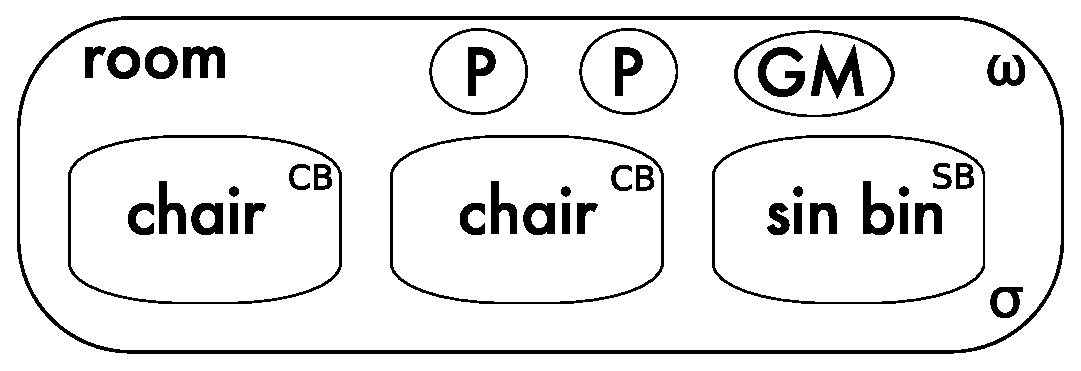
\includegraphics[scale=0.5]{gameenvbw}
  \caption{The Musical Chairs Environment}
  \label{fig:gameenv}
\end{figure}

The environ structure is represented graphically by Fig. \ref{fig:gameenv}
and in the calculus by the equation shown below.
\begin{equation}
\loc{room}{\nloc{chair}{\nil}{CB} \pc \nloc{chair}{\nil}{CB}
\pc \nloc{sinbin}{\nil}{SB} \pc P \pc P \pc GM}{\Omega}{\sigma}
\end{equation}
where $\nloc{m}{E}{F}$ is abbreviated from $\loc{m}{E}{F}{}$.  The
players themselves are represented by \emph{processes}.  This allows
them both to interact and to move between environs.  A gamesmaster
process is also introduced.  This doesn't play an active role in the
game itself, but is instead responsible for performing the
administrative duties of removing chairs from the game and controlling
player movement.  The process definitions are summarised in Table
\ref{tab:musicalchairs}, and make use of the derived syntax for a
clock prefix, $\sigma.P$, shown in \ref{clockcontrol}.  Their names
are shorthand for Chair Bouncer ($CB$), Sinbin Bouncer ($SB$), Games
Master x ($GMx$), Player ($P$), Moving Player ($MP$), Player in Chair
($PiC$), Player Leaving Chair ($PLC$) and Leaver ($L$).

\begin{table}[h]
  \caption{Summary of Processes and Derived Syntax for Musical Chairs}
  \label{tab:musicalchairs}
  \shrule
  \begin{align}
   CB &
    \eqdef 
    \mu X.(\bin.\bout.X + \bopen.\Omega) \label{chairb} \\
   SB &
    \eqdef 
    \mu X.\bin.X \label{sinb} \\
   GM1 &
    \eqdef 
    \sigma.GM2 \label{gmstage2} \\
    GM2 &
    \eqdef 
    \tntopen{chair}.GM3 \label{gmstage3} \\
   GM3 &
   \eqdef
   \sigma.GM4 \label{gmstage4} \\
   GM4 &
    \eqdef  
    \mu X.(\stimeout{\procin{sit}{chair}.X}{\sigma}{GM5}) \label{gmstage5} \\
   GM5 &
    \eqdef 
    \mu X.(\stimeout{\procin{leave}{sinbin}.X}{\sigma}{GM1}) \label{gmstage6}\\
    P &
    \eqdef 
    \sigma.\sigma.MP \label{player} \\
    MP &
    \eqdef
    \stimeout{sit.PiC}{\sigma}{L} \label{mplayer}\\
   PiC &
    \eqdef 
    \sigma.\sigma.PLC \label{pinchair} \\
   PLC &
   \eqdef
   \procout{stand}{chair}.\nil|stand.P \label{pleavechair} \\
   L &
    \eqdef 
    leave.\nil \label{loser} 
  \end{align}
  \shrule
\end{table}

The presence of music is signified by the ticks of a clock, $\sigma$.  A
tick from $\sigma$ is also used to represent the implicit
acknowledgement that everyone who can obtain a chair has done so, and
that the remaining player left in the room has lost.  With regard to the
bouncers of the environs, the room environ is not prone to either
destruction or the entry or exit of other environs, having a bouncer
simply equal to $\Omega$.  This retains the encapsulation of the model
as a single room environ, and prevents other processes or environs
from interfering with its behaviour.

The definition of appropriate bouncers is essential for the chairs
(\ref{chairb}) and the $sinbin$ (\ref{sinb}).  It is the chair bouncer
that enforces the implicit predicate that only one player may inhabit a
chair at any one time, while the $sinbin$ bouncer prevents players
leaving the $sinbin$ once they have entered.

To model stage one of the game, $n$ player processes and $n$ chair
environs are placed in the room.  The advantage of using NT for this
model is that the actual number of players or chairs is irrelevant.
They need not even be equal.  The calculus allows the creation of a
compositional semantics, as discussed in chapter \ref{introduction},
which works with any $n$.

For the purposes of demonstration, $n$ is assumed to be two to give the
following starting state:
\begin{equation}
  \loc{room}{\nloc{chair}{\nil}{CB} \pc \nloc{chair}{\nil}{CB} \pc 
   P \pc P \pc GM1}{\Omega}{\sigma}.
\end{equation}
The room and chairs appear as shown earlier.  The player
processes (\ref{player}) simply wait until two clock
cycles have passed, the end of each being signalled by a tick from
$\sigma$.  The intermittent period between the ticks (the second clock
cycle) represents the playing of the music.  

Stage two, where the music is started, is thus represented simply by the
first tick of $\sigma$,
\begin{equation}
\begin{aligned}
  & \loc{room}{\nloc{chair}{\nil}{CB} \pc \nloc{chair}{\nil}{CB} \pc 
   P \pc P \pc
   GM1}{\Omega}{\sigma} \\
 \lderives{\sigma}\ & \loc{room}{\nloc{chair}{\nil}{CB} \pc \nloc{chair}{\nil}{CB} \pc 
   \sigma.MP \pc \sigma.MP \pc
   GM2}{\Omega}{\sigma}
\end{aligned}
\end{equation}
which the gamesmaster ($GM1$ (\ref{gmstage2})) also waits for, before
evolving into $GM2$ (\ref{gmstage3}).  The second cycle, prior to the
music stopping, is used to remove a chair from the game.  Maximal
progress, as explained in section \ref{introduction}, ensures that this
occurs before the next clock tick, as the removal emits a high priority
action, $\topen$.  The transition from stage three to stage four is thus
as follows:
\begin{equation}
\begin{aligned}
& \loc{room}{\nloc{chair}{\nil}{CB} \pc \nloc{chair}{\nil}{CB} \pc 
   \sigma.MP \pc \sigma.MP \pc
   GM2}{\Omega}{\sigma} \\
 \lderives{\topen}\ & \loc{room}{\nloc{chair}{\nil}{CB} \pc 
   \sigma.MP \pc \sigma.MP \pc
   GM3}{\Omega}{\sigma}
\end{aligned}
\end{equation}
with one of the two chairs being chosen non-deterministically.
The second tick then occurs, leading in to stage five and the most
interesting part of the model.

\begin{equation}
\begin{aligned}
& \loc{room}{\nloc{chair}{\nil}{CB} \pc 
   \sigma.MP \pc \sigma.MP \pc
   GM3}{\Omega}{\sigma} \\
\lderives{\sigma}\ & \loc{room}{\nloc{chair}{\nil}{CB} \pc 
   MP \pc MP \pc
   GM4}{\Omega}{\sigma} \\
\end{aligned}
\end{equation}

The aim of stage five is to get as many player processes as possible
inside chair environs.  This is handled by again relying on maximal
progress to perform a form of broadcast that centres on mobile
actions, as briefly mentioned in \ref{procmob}.  Rather than sending a
signal to a number of recipients, a request to move into a chair (see
(\ref{gmstage5}) and (\ref{mplayer})) is delivered instead.

If a chair is available, then a player process will enter it (the
choice of chair and player is non-deterministic).  This will cause a
high priority action to occur, which takes precedence over the clock
tick.  Thus, when the clock eventually does tick, it is clear that no
more players can enter chairs. Using clocks in this manner makes the
system \emph{compositional}; in contrast to other models, players and
chairs can be added without requiring changes to the process
definitions.  In this running example, there are two players, but only
one chair, which results in a single $\tin$ transition:
\begin{equation}
\begin{aligned}
& \loc{room}{\nloc{chair}{\nil}{CB} \pc 
   MP \pc MP \pc
   GM4}{\Omega}{\sigma} \\
\lderives{\tin}\ & \loc{room}{\nloc{chair}{PiC}{\bout.CB} \pc 
   MP \pc
   GM4}{\Omega}{\sigma} \\
\end{aligned}
\end{equation}
that causes one of the $MP$ processes to move in to a
chair, and become a $PiC$ process.  This is followed by the
$\sigma$ transition, which marks the move to stage six.

\begin{equation}
\begin{aligned}
&  \loc{room}{\nloc{chair}{PiC}{\bout.CB} \pc 
   MP \pc
   GM4}{\Omega}{\sigma} \\
\lderives{\sigma}\ & \loc{room}{\nloc{chair}{\sigma.PLC}{\bout.CB} \pc 
   L \pc
   GM5}{\Omega}{\sigma} \\
\end{aligned}
\end{equation}

Both stage six and seven proceed in a similar way.  Stage six sees
essentially the same broadcasting behaviour applied to the losing
players (see (\ref{gmstage6}) and (\ref{loser})).  The difference is
that stage six demonstrates something which wouldn't be possible without
mobility: the broadcast is limited to those player processes which
remain in the room.  As communication between processes in different
environs is disallowed in NT, an implicit scoping of the broadcast
occurs.  In the example, stage six again sees just one $\topen$
transition:
\begin{equation}
\begin{aligned}
&  \loc{room}{\nloc{chair}{\sigma.PLC}{\bout.CB} \pc 
   L \pc
   GM5}{\Omega}{\sigma} \\
\lderives{\topen}\ & \loc{room}{\nloc{chair}{\sigma.PLC}{\bout.CB} \pc
   GM5}{\Omega}{\sigma} \\
\end{aligned}
\end{equation}
which results in the remaining $MP$ (now a losing process, $L$) moving
to the sinbin.  Due to space constraints, the sinbin environ is not
shown in the above derivations.  It may be factored in to the above as
follows:
\begin{equation}
\begin{aligned}
& \nloc{sinbin}{\nil}{SB} \pc L \pc GM5 \\
\lderives{\tin} & \nloc{sinbin}{\nil}{SB} \pc GM5
\end{aligned}
\end{equation}
 where the $L$ process evolves to become a simple $\nil$
process.  The broadcast is again terminated by a tick from $\sigma$,
\begin{equation}
\begin{aligned}
&  \loc{room}{\nloc{chair}{\sigma.PLC}{\bout.CB} \pc
   GM5}{\Omega}{\sigma} \\
\lderives{\sigma}\ & \loc{room}{\nloc{chair}{PLC}{\bout.CB} \pc
   GM1}{\Omega}{\sigma} 
\end{aligned}
\end{equation}
which, in this case, also signifies the music starting up again.  The
remaining players leave their chairs:
\begin{equation}
\begin{aligned}
& \loc{room}{\nloc{chair}{PLC}{\bout.CB} \pc
   GM1}{\Omega}{\sigma}   \\
\lderives{\tout}\ & \loc{room}{\nloc{chair}{\nil}{CB} \pc
   GM1 \pc P}{\Omega}{\sigma} 
\end{aligned}
\end{equation}
and the system essentially returns to the beginning, with $n -
1$ chairs and $n - 1$ players.

\section{A Prototypical Application in NT}
\label{app:nt}

Recall that in \ref{app:req} we specified a series of requirements for a music player application:

\begin{itemize}
\item The application should provide some form of interface with which
  the user can interact.
\item It should be able to take a wave file and return a sequence of
  sound data for playback.
\item It should be able to output the sound data through the speakers.
\item It should be able to generate a spectral analysis of the sound
  data as a form of visual feedback.
\end{itemize}

Now that we have our process calculus to work with, we can provide a formal design for this application,
which can then be converted directly into a real-world application using DynamiTE in the next chapter.

First, we will consider the reading of the wave file.  The simplest solution is:

\begin{equation}
  In \eqdef i.\mu X.\tau.\overline{o}.X
\end{equation}
\noindent where the filename is read in on $i$ and processed to
produce some sound data in the $\tau$ action.  The data is then output
on $o$.  We then recurse, continuing to produce more sound data and
output it on $o$\footnote{At some point, the $\tau$ process will reach
  the end of the file; there isn't an obvious way of representing this
  in the design so we just have to assume that, in the implementation,
  the internal $\tau$ process will terminate the thread running
  $In$.  We could use $X + \nil$ at the end, but then we are
  representing the end of the process as being non-deterministic, when
  it is in fact determined by the file.}.

From this, we can already determine some things about the other processes in the system:

\begin{itemize}
\item The interface ($\Intf$) must output on $\overline{i}$ to
  trigger $\In$ into starting to produce sound.
\item The speaker output ($\Out$) must read on $o$ to obtain the sound
  data and send it to the speakers.
\item The spectral analyser ($\Analy$) must read on $o$ to obtain the
  sound data and produce the visual feedback.
\end{itemize}

\noindent and definitions for $\Out$ and $\Analy$ follow fairly
trivally\footnote{We could represent these processes outputting on
  channels representing the speakers and display respectively, but in
  reality these are going to be system calls in the $\tau$ process,
  just as the $\tau$ in $\In$ performs reading and decoding operations
  on the file to produce sound data}:

\begin{equation}
\begin{aligned}
  & Out \eqdef o.\tau.\nil \\
  & Analy \eqdef o.\tau.\nil
\end{aligned}
\end{equation}

This already highlights one problem with the current $In$ process.
Both $\Out$ and $\Analy$ need to synchronise with it on the $o$ channel,
but it currently only performs one $\overline{o}$ action.  Thus, on
each loop within $\In$, one of the two will synchronise and the other
will miss out.

From \ref{tpl} and \ref{example}, we already know the best way to
solve this; with a timeout.  $\In$ needs to recurse over the
$\overline{o}$ action until it can no longer synchronise with a
reciepient, at which point it reads the next piece of sound data; this
is exactly the same logic as we employed for the compositional
broadcast agent in \ref{tpl}.  As a result, $\In$ now looks like this:

\begin{equation}
  In \eqdef i.\mu X.\tau.\mu W.\stimeout{\overline{o}.W}{\sigma}{X}
\end{equation}

\noindent We bind $W$ to $\timeout{\overline{o}.W}{\sigma}{X}$ so that
each time $\overline{o}$ is performed, we return to our original state.
When $\In$ is running in parallel with $\Out$ and $\Analy$:

\begin{equation}
  IntSys \eqdef i.\mu X.(\tau.\mu W.\stimeout{\overline{o}.W}{\sigma}{X} \pc o.\tau.\nil \pc o.\tau.\nil)
\end{equation}

\noindent the presence of both $o$ and $\overline{o}$ will allow a
$\tau$ transition to occur (rule $Par2$ in the semantics), which in
turn inhibits $\sigma$.  Once both have occurred, $\sigma$ transitions
can occur and will cause recursion to occur via the expansion of $X$.
Our structural congruence rules ($SCong$) mean that we can simply
discard the two $\nil$ processes left behind by $\Out$ and $\Analy$.

There is one remaining issue with this construction; the internal
$\tau$ actions of $\Out$ and $\Analy$ will also cause $\In$ to continue
to recurse on $W$ rather than reading the next piece of input.  The
solution to this is to also synchronise these two processes on
$\sigma$:

\begin{equation}
  Out \eqdef o.\stimeout{\Delta}{\sigma}{\tau.\nil}
\end{equation}

\noindent so that now, once input has been received on $o$, $\Out$
waits until $\sigma$ becomes unimpeded and is able to tick; $\Delta$
produces no transitions, so neither $STO2$ or $STO3$ can be applied,
while $STO1$ requires the absence of any high priority transitions,
which includes $\tau$ transitions. This should allow all three
processes to continue with their internal processing.  The same
definition can be applied to $\Analy$.

Of course, we could provide a much simpler solution by just performing
$\overline{o}$ twice.  The advantage of this solution, as we have
discussed before, is that we can add any number of other processes
that need to synchronise on $o$ without having to alter our definition
of $\In$.

All that remains to complete our definition of this system is to
define the interface.  This is simply a means of translating user
actions into calls to our internal system.  This can be as simple as:

\begin{equation}
  Intf \eqdef useri.(\overline{i}.\nil | IntSys)
\end{equation}

But what does $useri$ synchronise with?  This comes from the user and
is outside the system itself:

\begin{equation}
   \procin{begin}{player}.\nil \pc begin.\overline{useri}.\nil \pc \loc{player}{Intf}{\bin.\Omega}{\sigma}
\end{equation}

\noindent Our system is now encapsulated in an environ, $player$.  To
start the player, a client must enter $player$ and synchronise on
$useri$.  The bouncer of the $player$ environ allows only one process
to enter, by providing only one $\bin$ with which to synchronise.  The
clock $\sigma$ is hidden outside the environ so all the ticks from
within $player$ appear as silent actions to those outside (see
$LHd1$).  As all the other transitions performed by $\Intf$ will also
be silent actions, being a mix of internal $\tau$ actions and
synchronisations between $i$ and $o$, processes outside $player$ can
use the presence of these transitions to determine whether or not
$\Intf$ is active or not.

We have deliberately kept the design as simple as possible to make it
easier to digest and to reduce the complexity of the corresponding
implementation we will cover in \ref{app:dynamite} as part of our
discussion of DynamiTE.  There are many more things that could be
represented, not the least being a way of stopping playback once
begun!

\section{Conclusion}

In this chapter, we introduced our process calculus, Nomadic Time, the
first novel work in this thesis.  This extends the CaSE process
calculus of chapter \ref{case} with the notions of localities (see
\ref{migration}) and process migration (see \ref{ambientcalculus}).
We also added the notion of `bouncers', a security mechanism which
allows the number and type of mobility operations which may be
performed on an environ (our term for a locality in NT) to be defined.
The first half of the chapter demonstrated how each of these features
was layered onto the calculus, before finishing with its operational
semantics (\ref{ntsemantics}).  We then demonstrated how the calculus
may be used using two examples; the first (\ref{example}) aimed to
demonstrate each of the features of the calculus in action, while the
second (\ref{app:nt}) expanded on the application specified in
\ref{app:req} from a more real-world perspective.

In the next chapter, we show how Nomadic Time may be used to construct
a concurrent programming framework in the Java programming language.
We refer to this framework as the DynamiTE (Dynamic Theory Execution)
framework, and this forms the second novel work in this thesis.  We
then use this framework to implement a prototypical application, using
the design from \ref{app:nt} to construct corresponding Java classes
which meet the requirements in \ref{app:req}.  Finally, we cover some
other existing attempts to provide implementations of process calculi.


% The Concurrent Object Framework
% Thesis: DynamiTE
% Author: Andrew Hughes

\chapter{The DynamiTE Framework}
\label{dynamite}

\section{Introduction}

In this chapter, we introduce DynamiTE, the Dynamic Theory Execution
framework.  This provides the solution we first proposed in
\ref{solution}, using the Nomadic Time (NT) calculus introduced in
\ref{nt} and \ref{tnt} as a foundation for application development.
Through using DynamiTE, programmers compose NT processes, realised as
Java objects, to create a working system.  The framework handles
running these processes, in parallel if necessary, and negotiates the
communication between them.  Both features are provided by leveraging
existing facilities in the underlying Java virtual machine and class
library.

Over the course of this chapter, we will describe how NT processes are
mapped onto Java objects (see \ref{dyn:maptheory}) and then show how
DynamiTE can be used to create an implementation of the application we
introduced in \ref{protoapp} (see \ref{app:dynamite}).  But first, we
discuss why we chose Java as the host language for DynamiTE and what
advantages and disadvantages this brings to its implementation.

\section{Why Java?}

The first implementation of the Java programming language was released
in 1995 by Sun Microsystems.  It takes the form of a block structured
language with a syntax akin to C or C++.  However, unlike programs
written in those languages, Java applications tend to be compiled to
platform-independent Java bytecodes which are then executed by a Java
Virtual Machine or JVM.  This allows the same Java program to be
executed on multiple platforms without the need for recompilation.
With this new operating environment comes the removal of a number of
features found in Java's predecessors and the restriction of others,
with the aim of creating a safer and more portable language:

\begin{itemize}
\item \textbf{No pointer manipulation}.  All primitive types in Java
  (integer, floating point numbers, booleans and single characters)
  are passed by value.  All objects are stored and passed as pointers
  or references to their location in memory.  These pointers are
  immutable, removing the ability to perform pointer arthimetic
  (e.g. for iterating over arrays) and with it, a host of problems
  inherent with inappropriate memory access.  For example, attempts to
  use a \texttt{null} pointer are caught by the virtual machine and
  produce a checked exception, rather than causing a segmentation
  fault which brings down the entire process.
\item \textbf{All arrays are bounds checked}.  A major cause of errors
  and security issues in C and C++ programs is the possibility of
  buffer overflows, where programs write to memory beyond the end of
  an array.  In Java, such errors are prevented by the virtual
  machine; any attempt to access an index outside the bounds of an
  array causes a checked exception to be thrown and direct access to
  the array's memory is forbidden by the lack of pointer manipulation.
\item \textbf{All memory management is performed by a garbage
  collector}.  While allowing manual memory management allows the
  programmer greater control, it leads to an equivalent to the issue
  we saw with semaphores in \ref{semaphores}; every allocation must be
  paired with a later deallocation to avoid the possibility of an
  application leaking memory.  The problem is even more pronounced
  with regard to memory management as, while the acquisition and
  release of a lock tend to occur in close proximity to one another,
  allocation and deallocation can occur in quite disparate parts of
  the application.  In Java, memory is instead managed by a
  \emph{garbage collector} which allocates memory for objects as
  needed and periodically reclaims those that are no longer
  referenced.  The downside of this is that the garbage collector has
  to use processor time to perform its scans which would otherwise be
  used by the application.  However, as new garbage collection
  techniques, such as concurrent and generational collectors, become
  prevalent, this disadvantage is further outweighed by the prospect
  of chasing memory leaks.
\item \textbf{Lack of unsigned types}.  All integer types in Java use
  a bit to store the sign of the value, with no equivalent unsigned
  types that instead use this bit to store larger values.  This makes
  bitwise operations (and (\texttt{\&}), or(\texttt{|}) and
  not(\texttt{\~})) more inefficient as they need to operate on the
  type one size above (bytes ($2^8$) on shorts ($2^{16}$), shorts on
  ints ($2^{32}$), etc.).  Indeed, section 15.22.1 of the Java
  language specification\cite{javaspec} states that \emph{binary
    numeric promotion} (as defined in 5.6.2) should be applied to the
  operands, causing them to be converted to integer or long integer
  levels of precision before the operation is performed.  Thus, it
  logically follows that it is impossible to work with unsigned long
  integers ($2^64$) without resorting to the overhead of a class which
  implements arbitrary precision integers, such as
  \texttt{java.lang.BigInteger}.  Unsigned types continue to be
  proposed for addition to the Java language, but no such extension is
  scheduled for the next release (Java 7).
\end{itemize}

Although these changes are made at the expense of flexibility for the
programmer and possible efficency gains, they save time overall in
chasing bugs caused by memory allocation errors, buffer overflows or
leaks.  Besides, the Java Native Interface (JNI) can be used to
implement certain methods in C, should the need arise.  Many of the
methods provided by the Java class library do just that, usually to
make use of a platform-specific application programming interface
(API).  Doing so has some overhead and means losing the safety and
memory management benefits of Java, but is possible where necessary.

Performance has been a common criticism of Java, not just because of
these features but also because the Java bytecodes it uses must be
either interpreted or compiled into native code at run time.  This is
much less of an issue than it once was, due to advances in virtual
machine design and Just-In-Time (JIT) compilation techniques.
Theoretically, JIT compilation should eventually exceed the
performance of code compiled Ahead-Of-Time (AOT) as it can take
advantage of information only available at runtime.  This includes
knowing the exact platform on which the code will execute and being
able to make better optimisations based on statistics gathered through
execution (e.g. better branch prediction).  For example, HotSpot, the
virtual machine used by Sun's implementation of Java, only uses the
JIT compiler to create native code when it believes the code is used
enough (`hot' enough) to make doing so worthwhile.

Of these changes, the absence of unsigned types is the only one that
seems to have no advantage, other than simplifing the language.  Many
file formats and network protocols include unsigned types, so working
with them in Java becomes harder than is necessary.  Although their
absence may have made sense in earlier versions of the language, the
complexity of understanding unsigned arithmetic now seems trivial when
compared with the existential type system and its lack of reification
which was introduced by the addition of `\emph{generics}' in Java 5.
We thus hope that they may make an appearance in Java 8.

\subsection{Concurrency Provision}

From the perspective of implementing DynamiTE, one advantage of Java
is its broad support for concurrency.  Java is one of the few
languages to have an implementation of \emph{monitors}, a feature we
demonstrated in \ref{semaphores}.  It has also had support for threads
from the very beginning, with support as a core part of the virtual
machine rather than as an auxillary library (the approach used for C).
Java's platform independence means that the same threading constructs
and semantics, as mandated by the VM specification\cite{vmspec}, can
be used across all operating systems supported by a Java virtual
machine.  The actual implementation is provided by the virtual machine
and class library, which may either map them on to native threads or
provide \emph{green} threads, where the virtual machine itself creates
and schedules threads.  The main disadvantage of the latter is that
blocking calls to the operating system performed by one thread will
cause the virtual machine and all its threads to be blocked; as the
system is unaware of the presence of the threads, its only option is
to block the entire VM process.  Green threads are however much faster
to create and synchronise, as everything takes place within the VM.
They can also match the required thread semantics exactly, rather than
having to map those provided by the operating system's threads.  While
earlier versions of Sun's implementation used green threads, native
threads are now used on all supported platforms.

The result of this early adoption of multithreading is that the
implementation in Java is reasonably mature and well-tested.  With
Java 5, this support was greatly expanded as a result of research led
by Doug Lea and incorporated into the Java platform via JSR166 and the
\texttt{java.util.concurrent} packages \cite{jsr166, concpractice}.

The extensions provided by JSR166 take the form of a host of new
classes, backed by support in the virtual machine.  The Java language
itself is not altered.  It provides support for:

\begin{itemize}
\item \textbf{Atomic Variables}.  These provide replacements for
  integer, long integer and reference fields which can be updated in
  an atomic fashion, are safer than \texttt{volatile} variables and
  more efficient than locking.  The Java memory model allows
  operations which alter the value of normal fields to be reordered by
  the VM as a form of optimisation, as long as this reordering is not
  visible from within the same thread.  However, this means that other
  threads may see the changes in the wrong order or not at all.
  Marking a field as \texttt{volatile} makes the VM aware that it may
  be accessed by multiple threads, causing updates to be made visible
  to all threads immediately.  However, \texttt{volatile} fields are
  still prone to race conditions when used in non-atomic operations
  such as incrementing a value or performing a conditional
  update\footnote{e.g. in \texttt{if (x == 4) x = 5}, it is possible
    for \texttt{x}'s value to have been changed by another thread
    before the assignment but after the comparison}.  The usual
  solution is to obtain a lock on the class every time the variable is
  altered; this provides both the update guarantees of a
  \texttt{volatile} variable and blocks other threads trying to obtain
  the same lock.  Atomic variables provide an alternate solution by
  allowing the processor's CAS operation (see \ref{semaphores}) to be
  used.  This is usually more efficient than locking the entire class,
  which will involve the VM performing a CAS operation on the lock at
  some point anyway.  While locking takes a pessimistic approach to
  thread safety by blocking all other threads, CAS operations are
  optimistic; the update is attempted, and if it fails, we try again
  until it succeeds.  Implementing such a check successfully is even
  more prone to error than locking, as the programmer has to ensure
  they check the result of the CAS and loop accordingly, but it is
  usually much more efficient when contention is low.  With the
  addition of atomic variables to Java, programmers now have the
  choice of using either.
  \item \textbf{Explicit Locks}.  As we saw in \ref{semaphores}, Java
    has implicit reentrant locking via the \texttt{synchronised}
    keyword.  Their use, however, is limited; there is only one lock
    per class, so all its variables must be protected by the same
    lock, and threads are always blocked until they either acquire the
    lock or the thread is interrupted by \texttt{Thread.interrupt()}.
    The \texttt{ReentrantLock} class provides a more advanced version
    with the following additional features:
    \begin{itemize}
      \item \texttt{tryLock()} can be called to perform a non-blocking
        acquisition of the lock.  It immediately returns with
        \texttt{true} if the lock was acquired, and \texttt{false} if
        it wasn't.
      \item \texttt{tryLock(long, TimeUnit)} can be called to perform
        a timed acquisition.  If the lock is available, it acquires it
        and returns immediately.  Otherwise, it blocks.  However,
        unlike the implicit lock provision and the \texttt{lock()}
        method, it will become unblocked after the given timeout and
        return \texttt{false}.
        \item The lock can operate in a fair mode, where threads
          acquire the lock in the order they requested it.  Both
          implicit and explicit locks default to unfair behaviour,
          which permits \emph{barging} if a new thread happens to
          request a lock when it is unheld.  Unfair locks are much
          faster\footnote{If threads are not allowed to jump the
            queue, then we end up blocking and descheduling a thread
            which could have quite happily acquired the lock but isn't
            allowed to do so because of the fairness policy}, but
          fairness is sometimes needed to ensure correctness.
    \end{itemize}
    A class can have multiple instances of an explicit lock, just like
    any other variable, and this benefit is utilised by
    \texttt{ReentrantReadWriteLock}.  This class provides both a
    shared (\textbf{read}) lock and an exclusive (\textbf{write})
    lock.  Multiple threads can acquire the read lock, but to acquire
    the write lock, both locks must be unheld.  This can be used to
    make classes more efficient when compared with the brute force
    approach of enforcing mutual exclusion for all operations.  For
    example, a collection class can allow multiple threads to read
    values as long as there is no thread altering the collection.
    Both locks, and other implementations such as \texttt{Semaphore},
    are based on \texttt{AbstractQueuedSynchronizer}\cite{aqs} which
    provides a common framework thread queues.
    \item \textbf{Explicit Condition Queues}.  As in the case of
      locks, Java already has its own implicit condition queues,
      accessible via the \texttt{wait}, \texttt{notify} and
      \texttt{notifyAll} methods.  These also have similar limitations
      to the implicit locks; only one queue is available per class and
      either one or all threads must be notified.  With only one
      condition queue, the usability of \texttt{notify} to alert a
      single thread is extremely limited; using it is dangerous if
      there is more than one condition as the wrong thread may be
      awoken, and it is inefficient unless a change in the condition
      means that one and only one thread may proceed.  The former can
      be observed in the buffer example of \ref{semaphores} where
      there are two conditions: \texttt{used == BUFFER\_SIZE} and
      \texttt{used == 0}. The latter is observable in a `gate'
      scenario where multiple threads queue up waiting for a condition
      to hold, and then all proceed when it does.  Explicit condition
      queues address these issues by allowing a class to have multiple
      condition queues.  Each \texttt{Condition} is obtained from a
      \texttt{Lock} by a call to \texttt{Lock.newCondition} and that
      same lock must be held when calling its methods.  In the buffer
      example, the synchronized blocks would be replaced by the use of
      explicit locks and the calls to \texttt{wait} and
      \texttt{notifyAll} by \texttt{await} and \texttt{signal} calls
      on one of two \texttt{Condition} objects.  The \texttt{signal}
      method can now be used rather than \texttt{signalAll}, awakening
      just one thread, as we know the thread will be waiting for the
      condition whose state has changed and no other.  This avoids
      waking all threads and having all but one go back to sleep.
    \item \textbf{Executors and Thread Pools}.  The new classes
      provide a framework for executing tasks in the form of the
      \texttt{Executor} interface.  This decouples the process of
      submitting a task from how it is executed.  Tasks (in the form of an object which implements the \texttt{Runnable} interface) are submitted to an \texttt{Executor} instance, and then performed in a manner determined by the \texttt{Executor} implementation.  The \texttt{Executors} class provides a number of pre-defined instances:
      \begin{itemize}
        \item A single thread executor, which performs tasks sequentially.
        \item An executor with a fixed size pool of threads.
        \item An executor with an unbounded pool that grows and shrinks as demand allows.
        \item An executor with a fixed size pool of threads and delayed or periodic task execution.
      \end{itemize}
      The programmer is also, of course, free to define their own
      implementation.  This feature is very useful for implementing
      parallel composition in DynamiTE as each process may be
      submitted to an executor, the choice of which is left up to the
      user of the framework.
    \item \textbf{New Collections}.  The standard Java collections
      apply an all-or-nothing approach to thread safety; either the
      instance is unsafe for multithreaded use (as with instances of
      the Java 1.2 classes -- \texttt{HashMap}, \texttt{ArrayList},
      etc.) or every method call locks the class (as with the legacy
      classes such as \texttt{Vector} and \texttt{Hashtable} or the
      1.2 classes when wrapped by the \texttt{synchronizedX} methods
      in \texttt{Collections}).  The JSR166 extensions provide a new
      set of collections which utilise the features listed above.  For
      example, \texttt{ConcurrentHashMap} provides a hash map which
      utilises \emph{lock striping}; the map is protected by multiple
      read and write locks which protect only a segment of the whole
      map each.  Thus, not only can multiple readers access the map
      concurrently, but it may be possible to perform multiple writes
      concurrently if they effect different areas of the map.  The new
      collections also include various \texttt{BlockingQueue}
      implementations, which implement the producer-consumer model we
      demonstrated with the buffer example in \ref{semaphores}.  One
      such implementation is \texttt{SynchronousQueue} which closely
      matches the semantics of synchronous channels in Nomadic Time;
      it has no storage so a thread performing a \texttt{put} blocks
      until a receiving thread calls \texttt{take}.
\end{itemize}

With these additions, the programmer is given a lot of control and
flexibility when implementing concurrent programs in Java, and we will
leverage many of these features when implementing DynamiTE.  Having
essential components such as locks and concurrent collections already
available and well tested makes it much easier to meet the
requirements of the framework.

Other languages are not so lucky.  In C and C++, threads are provided
by an operating system library and thus vary depending on platform.
The POSIX standard for threads attempts to overcome this by providing
a standard threading interface and semantics for POSIX systems.  While
POSIX-based systems including GNU/Linux, Solaris, FreeBSD and Mac OS X
all provide implementations. the problem remains with systems that do
not provide such by default, notably Microsoft Windows.

Haskell has been slow to introduce threading support.  Although the
Concurrent Haskell\cite{conchaskell} extension was originally proposed
in 1996, it does not form part of the Haskell 98 standard and the GHC
documentation still lists it as experimental.  Both Hugs and the
Glasgow Haskell Compiler (GHC), the two main implementations of
Haskell, provide an implementation of Concurrent Haskell's
\texttt{Control.Concurrent} module, they do so using green threads.
As mentioned above, while these are faster than native threads,
blocking calls to the operating system, such as I/O, will cause all
threads to be blocked.  A workaround is provided in GHC when it is
built with the \texttt{-threaded} option; it uses a pool of worker
threads to execute Haskell code and switches to a new one when a
\texttt{safe} foreign call is made.  It also allows native threads via
\texttt{forkOS} when built in this manner.  As with C, this makes
Haskell's thread behaviour dependent on the underlying system as
opposed to providing a standard set of operations and semantics;
whether threads are provided and how well they perform depends
entirely on which implementation of Haskell is being used.

However, functional languages in general should be a good basis for
concurrency.  They already operate in a task-oriented manner through
\emph{pure functions}; data is fed in, manipulated as desired and the
result output without altering memory.  Those that do alter memory,
and thus could lead to concurrency issues, are clearly denoted
(e.g. by monads in Haskell), reducing the amount of code that has to
be checked for race conditions.

It is thus a pity that they are not more widely used and their
concurrency facilities not more well developed.  This is changing,
however.  GHC has recently been extended with support for Software
Transactional Memory (STM) \cite{haskellstm}, which provides a new
\texttt{atomic} function and \texttt{STM} monad for implementing
transactions.  The STM logs all actions and then performs a single
atomic commit, provided there are no conflicts with other updates.
This allows Haskell programmers to compose new atomic transactions
from others, and moves the need to ensure atomicity away from each
individual function to the caller, who can only invoke them from
within an atomic environment.

Erlang\cite{erlang} is another interesting case, as both it and
DynamiTE focus on message passing between processes as opposed to
shared data and locking.  Erlang differs in that it operates
asynchronously, collecting messages in a mailbox on a per-process
basis and filtering which ones are received in any one operation.
However, synchronous delivery can be implemented by requiring messages
to be acknowledged.  The main limitation of current Erlang
implementations is that they use green processes; unlike green
threads, these don't share state but they do have the same downside
that a blocking system call from one will cause them all to become
blocked by the system.

Both Erlang and Haskell provide an interesting environment in which to
implement a framework like DynamiTE.  Indeed, we hope that the
majority of the design explained here in \ref{dyn:maptheory} can be
applied to most languages with sufficient threading support.  However,
there is another reason for our choice of Java as the initial
prototype language.

\subsection{Popularity}

Popularity is rarely a good reason to do anything but, in combatting
developer inertia, it is a good weapon to have.  The simple fact is
that most of today's developers know Java and sometimes little else;
it (or its close relative, C\#) is taught as part of most computer
science degrees and is used as the language of choice for many
applications, especially in the area of enterprise web applications.

As we discussed in \ref{solution}, easing the barriers for adoption is
an essential aspect in influencing developers to try something new.
With DynamiTE, we are already advocating the idea of using message
passing rather than state manipulation to Java developers, a body of
programmers who will generally be more familiar with object-oriented
design techniques which focus on manipulating data.  Adding the
prospect of learning an entirely new language is not going to help our
case, and we believe this to be the main reason other solutions have
not moved far beyond their academic roots.  Instead, DynamiTE is
developed as a Java class library like any other, which leverages
standard features of the Java platform and which can be further
developed by the very people that use it.

We will be the first to admit that Java has issues; its age means that
with hindsight many design decisions can now be seen as flawed and
attempting to change this leads us to consider the bane of all
programming languages -- backwards compatibility.  Most features, good
or bad, are now enshrined in the language and further development
rightly takes a conservative attitude to avoid breaking the huge body
of existing code already in use.  This means that APIs are deprecated
rather than removed, causing the class library to become more bloated
than ever, and new language features such as generics take years to
appear and even then have to be limited.  No consensus has yet been
reached on how closures should be implemented, so they will not appear
in Java 7 either.  These issues are here to stay; Java is unlikely to
ever have a type system as advanced as that of most functional
languages or a separation between pure and impure functions.  But with
these come maturity and a vast body of developers which we believe to
be far more useful in achieving our goal than the possibilities of a
perfect but niche language.

\section{Mapping Theory to Practicality}
\label{dyn:maptheory}

In this section, we show how the constructs of NT introduced in
chapter \ref{nt} are mapped on to Java classes by the DynamiTE
framework.  Within DynamiTE, developers can create concurrent
applications simply by implementing the specific behaviour they
require in appropriate subclasses.  Recall the syntax of NT from \ref{eqn:tnt-syntax}:

\begin{equation}
  \begin{aligned}
    \expr, \exprb \quad \mathrel{::=} \quad &
      \nil  \mid
      \Omega \mid
      \Delta \mid
      \Delta_{\sigma} \mid
      \alpha . \expr  \mid
      \expr + \exprb \mid
      \expr \mathrel{\!|\!} \exprb \mid
      \timeout{\expr}{\sigma}{\exprb} \mid \\
    & \stimeout{\expr}{\sigma}{\exprb} \mid 
      \mu X . \expr \mid
      X \mid 
      \expr \res{A} \mid
      \locv{m}{\expr}{\exprb}{\vec{\sigma}} \mid
      \ambop . \expr \\
   \ambop \quad \mathrel{::=} \quad & \tntin{m} \mid \tntout{m} \mid \tntopen{m} \mid
      \procin{\beta}{m} \mid \procout{\beta}{m} \mid \bin \mid
      \bout \mid \bopen
   \end{aligned}
\end{equation}

Each syntactic construct is mapped
to an appropriate Java class, which provides the required
functionality and relates to others via a common \texttt{Process}
superclass.  Operation follows a top-down approach; the complete
system is represented by a single instance of one of these classes
which, in most cases, will be an operator that composes together
further instances as appropriate.

The simplest \texttt{Process} subclass is the representation of $\nil$,
realised as a class \texttt{Nil} which provides process termination.
The internal action $\tau$ is realised as an abstract class \texttt{Tau}
and this is where the user can implement arbitrary sequential behaviour
as required, by providing a subclass. The observable actions form part
of the channel subsystem, described in \ref{dyn:channels}.

The $+$ operator is implemented as a class which contains a list of
subprocesses from which one is chosen at random.  The action to perform
is computed by traversing the hierarchy, so restriction is simply a
matter of providing appropriate filtering, thus preventing the
restricted names from travelling further up the hierarchy.

More interesting is the \texttt{Par} class which implements the $\mid$
operator, as it must allow its subprocesses to operate concurrently.
The most obvious way to achieve this is by mapping individual processes
onto Java threads.  This also means that data can be stored with the
process by means of thread-local variables.  However, we are keen to
offer flexibility in how the individual features of the framework are
implemented.  Java thread mapping is only one way in which concurrent
processing may be implemented and so we abstract away \texttt{Par} from
the threading implementation as much as possible, thus allowing it to be
replaced by other implementations at a later date.  For example,
concurrent processing could also be provided by distinct processes
spawned by the VM or a more complex distributed solution may become
apparent.

\subsection{The Channel Abstraction}
\label{dyn:channels}

In the same vein, the implementation of synchronisation channels is
abstracted in such as way as to allow for differing implementations.
Here, the provision of multiple implementations is more prevalent and so
a plugin mechanism is already present.  Fortunately, Java already has
plenty of support for plugin based frameworks (imaging and sound already
being implemented in this fashion) and the new
\texttt{java.util.ServiceLoader} API provided in 1.6 makes this simpler
still.  This allows the user to have freedom of choice with respect to
their chosen channel implementation, which may even be further extended
by their own or third-party plugins.

At its simplest, DynamiTE provides a way of testing NT processes and
ensuring they perform as expected.  In this respect, the simplest
channel plugin is a dummy channel, which need do nothing more than
simply exist.  More complex solutions are of course possible and are
needed to make the framework both usable and interesting.  

Although currently there is no realisation of data within the formal
layer of the calculus, this only matters to the extent that we wish
transmitted data to alter the constructs themselves via
substitution\footnote{The $\pi$ calculus \cite{picalctutorial} is an
obvious example of such behaviour, which goes to the extreme of not only
allowing data to be transferred but also references to channels which
can then later be used in the language constructs.  This, in essence,
provides the form of mobility present in the $\pi$ calculus.}.  Data can
be transferred between processes and used within internal actions
without having to be explicitly realised at the formal level.  There are
a multitude of ways of implementing data transfer, ranging from simple
mechanisms like files and sockets to more full-blown interprocess
communication protocols such as Java's Remote Method Invocation (RMI),
the Common Object Request Broker Architecture (CORBA) and web services.
The plugin nature of the channel architecture means that any of these
possibilities may be used and more besides.

While the implementations of the channels themselves can provide the
input and output mechanisms, interoperability between the two has to
take place at a higher level.  Thus, the onus is on the parallel
implementation, \texttt{Par}, to co-ordinate the communication between
the two, by virtue of discovering which names are exposed at the point
of composition.

A possible simplification becomes apparent here, as some implementations
may make use of channel naming.  For example, if the channel name refers
to a host and port for a TCP/IP implementation, then the sender need
only try and connect to see if a recipient is available.  Channel names
are assumed to be unique, so such a mapping is possible.  However, they
are not unique to a particular process, making it perfectly plausible
for the channel name to occur simultaneously on multiple processes and
thus for a competition to occur.  There is also the issue of whether
they can actually `see' each other, according to the constraints of the
calculus, so the decision should still be left to an appropriate
parallel composition operator.

\subsection{Signalling}
\label{dyn:signalling}

One of the most interesting parts of the DynamiTE framework is the
implementation of clock signals.  While there have been other attempts
to produce frameworks or languages based on process calculi (see section
\ref{dyn:relatedwork}), we believe that the rendering of discrete time into
such a context is novel.

The first question to answer when attempting to perform such a
translation is where to actually locate the clocks.  Within NT, the
obvious answer is within each environ, as these are responsible for
providing the division between processes which can observe clock ticks
and those which can not.  For example, the following environ
\begin{displaymath}
\loc{m}{P}{\Omega}{\sigma}
\end{displaymath}
would be realised as an instance of the \texttt{Environ} class with the
name $m$.  This instance would maintain a reference to the process $P$
with which it interacts.  Not only is the execution of $P$ controlled by
the environ (as with the implementations of $+$ and $\mid$ above), but
it also controls when and how the ticks of $\sigma$ reach $P$.

Recall our earlier description of the calculus, where we mentioned how
clock ticks are always pre-empted by high priority actions, which may
arise either from explicit internal actions denoted by $\tau$, implicit
internal actions caused by synchronisation or movement.  So, in order
for the environ to know whether to propagate a clock tick to the
process, it must first probe it to find out whether such a high priority
action is pending.  Clock ticks may also be prevented by the $\Delta$
and $\Delta_\sigma$ constructs, so these must also be checked for.

Both can actually be achieved in one transaction by making the probe the
clock tick.  The clock tick is sent down the process hierarchy until it
reaches a point at which a decision can be made as to whether the tick
should occur or not.  If the tick can occur, it is propagated back up
the hierarchy, eventually stopping when it reaches its host environ
again.  The host environ can be determined by the set of clocks
associated with each environ, which is also used to calculate the
signals to be propagated initially.  If the clock is not allowed to
tick, then the actual action performed is sent instead.

This algorithm is best explained by a couple of prototypical examples.
First, consider 
\begin{displaymath}
\loc{m}{a.\nil + b.\nil}{\Omega}{\sigma}
\end{displaymath}
where the process inside $m$ has no $\tau$ actions, synchronisations,
mobility or clock stop operators, and thus clearly allows the clock
$\sigma$ to tick.  The environ $m$ iterates over its set of clocks (here
just $\sigma$), and sends a tick from each to its process, $a.\nil +
b.\nil$.

This process is realised by an instance of the \texttt{Sum} class, which
composes the two processes together.  A clock can only tick over the
summation operator if it can tick over both sides, so the result from
this instance is simply the result of combining the return value from
probing each of the constituent processes.

Both $a.\nil$ and $b.\nil$ are implemented using instances of the
\texttt{Prefix} class, which composes a \texttt{Channel}\footnote{An
abstract class, instances of which are provided by the channel
architecture described in \ref{dyn:channels}} or \texttt{Tau} instance
(unified by the \texttt{Action} class) with another instance of a
\texttt{Process} subclass.  In determining whether a clock can tick, it
first checks that the action is a channel rather than a \texttt{Tau}
instance (which would pre-empt the clock), and then probes the
\texttt{Process} instance.  In both these simple cases, this is an
instance of \texttt{Nil}, which allows clock ticks.

Having determined that the clock may tick, each nested call returns with
the $\sigma$ clock tick, thus propagating it up to the original call in
the environ $m$.  Having seen how this operates for a process that can
tick, it is simple to see how it differs when something prevents the
clock from ticking.  If any part of the query returns something other
than a clock tick, this will be propagated upwards in preference.

Consider what happens if $a.\nil$ is changed to $\tau.\nil$.  The
left-hand side of the summation will receive the $\tau$ action from the
\texttt{Prefix} instance, which then takes priority over the $\sigma$
from the right-hand side and is propagated to the environ, $m$.  This is
the case in any situation where the $\sigma$ is required to compete
against an action, a $\tau$ or a mobility primitive.  The clock stop
operators behave slightly differently in that they don't replace the
action, but instead mark the $\sigma$ action as \emph{stopped}.

Note that a similar method of determining the presence of clock ticks
must take place to handle the \texttt{STimeout} and \texttt{FTimeout}
classes.  Both sides of the timeout are inspected, and behaviour
determined as follows:
\begin{enumerate}
\item If the left-hand side can perform a high-priority action, it will
      be allowed to proceed and the right-hand side need not be
      considered.
\item Otherwise, the possible actions include unpaired actions (such as
      $a$ and $b$) and clock ticks (both from the clock involved in the
      timeout and from other clocks), one of which is chosen to be
      performed.
\item Once the chosen action has been performed, the timeout instance
      will be replaced as appropriate (see chapter \ref{nt}). 
\end{enumerate}

\subsection{Structural Changes}
\label{dyn:structchange}

The \texttt{Environ} class also places a central role in providing
system structure.  In chapter \ref{nt}, we described how
processes are organised into environs and the way communication is
limited to its bounds.  Within DynamiTE, one possible use of environs
is to map them to physical or virtual hosts.  While a simple testing
solution can execute the entire system on a single platform, environs
provide a natural form of process distribution which can be leveraged by
the framework.

This does however give the initial impression that structural mobility
will become very inefficient, if hosts are expected to interact to
determine the feasibility of a move and then actually change position
during execution.  In reality, these issues are minimal.  An inward
movement is always in relation to a sibling, while an outward movement
concerns some parent environ.  As the structure of environs is expected
to closely match the actual physical structure of the hosts, such
interactions should be relatively low cost to perform.  Also, a
structural movement does not change the contents of the moving environ,
only its context.  Thus, only later communication with surrounding
environs is affected.  For example, it may have been able to see a
sibling environ before the movement, but is now inside this environ and
can receive clock ticks emitted by it.

If hosts do not physically move, then what is the point in allowing such
structural changes?  The change in clock signalling just mentioned is
one effect.  In addition, we also make provision for contextual data to
be stored at the environ level, in addition to that stored local to a
particular thread, and transferred via channels.  This gives additional
purpose to the use of structural mobility and process migration, which
we describe next.

\subsection{Migration}
\label{dyn:migration}

The final aspect of DynamiTE that we describe here is the migration of a
process from one environ to another, which occurs both as a result of
using one of the process mobility operators and from the behaviour of
$\tntopen$.  This is perhaps one of the most interesting aspects, as it
represents the movement of code from one environment to another,
possibly located in a different physical location.

Migrating an active process is not a simple operation.  Not only must
any remaining code to be executed be transferred, but any local data
must also migrate.  NT does allow us to achieve a significant amount of
simplification here.  The transferred process is already separated from
other code within the system by virtue of the moving process being in
the form of a \texttt{Prefix} instance.  When the action is matched to
the one used for the mobility operation, the \texttt{Process} instance
is transferred to its new location.  There is no necessity to deal with
code that is currently being executed.

As with concurrency and channel operation, how movement is achieved is
designed to be flexible, with provision being made for distribution and
code migration to be implemented in different ways.  One of the most
obvious ways is to serialise the \texttt{Process} instance and
reconstitute it at its destination.  Migrating a process should then
just be a case of transmitting the serialised instance, followed by any
local data, and beginning execution at the destination.  However, this
is one area in which we expect further study of the existing literature
to enlighten us with more sophisticated ways of achieving such
migration.

\section{A Prototypical Application in DynamiTE}
\label{app:dynamite}
                                   
\section{Related Work}
\label{dyn:relatedwork}

There has already been a significant body of research into providing
concurrent frameworks, including those based on process calculi.
However, we believe our work to be novel in approaching the
implementation of both global discrete time, via clock signalling, and
mobility.

The $\pi$ calculus has been the subject of much of this work, primarily
due to its status as the most prevalant mobile process calculus.  Obliq
\cite{obliq} and Pict \cite{daveturner:phd} are both programming
languages with semantics founded in the $\pi$ calculus, while Nomadic
Pict \cite{wojciechowski:phd} takes this further, introducing
distribution not usually present in the $\pi$ calculus.  Within research
related to the ambient calculus, a machine framework (PAN
cite{sangiorgi:safeambientsmachine}) has been developed and
implemented.  Process calculi, such as the Seal calculus \cite{seal}
have also been developed specifically to provide a formal framework for
a distributed implementation.
%The $\pi$ calculus has been the subject of much of this work, primarily
%due to its status as the most prevalent mobile process calculus.  Obliq
%\cite{obliq} and Pict \cite{daveturner:phd} are both programming
%languages with semantics founded in the $\pi$ calculus, while a machine
%framework (PAN \cite{sangiorgi:safeambientsmachine}) has been developed
%and implemented for the ambient calculus.

\section{Conclusion}


% Types
% Thesis: Typed Nomadic Time
% Author: Andrew Hughes

\chapter{Typed Nomadic Time}
\label{tnt}

\section{Introduction}

A type system is a common addition to a process calculus.  This is
especially true, when the intended use of the calculus is as the basis
for a programming language or a distributed system, which is the case
here.  In this final chapter of original research, we demonstrate how
Nomadic Time may be extended with a type system based on the notion of
groups (see \ref{typesys}) and how this may then be used in DynamiTE
(see \ref{dyn:type}).  Each process is assigned to a group, which then
determines which environs it may \emph{reside} in, \emph{open},
\emph{leave} or \emph{enter}.

Before we enter into the technicalities of how this system is
implemented, we first present some existing type systems used in other
process calculi, including the origins of this group-based system.

\section{Existing Typed Calculi}
\label{typedcalculi}

Type systems can be used to restrict the calculus in ways that aren't
always possible via mere manipulation of the syntax and semantics.
Adding a type system can be as simple as formalising implicit notions,
such as the use of $\ambin{m}$ as a capability and not as part of a
path \cite{ambienttypes} or the fact that the $x$ in $x(y)$ should be
represent a link and not a mere value \cite{sangiorgi:types-or}.  It
may also provide more complex intuitions, by distinguishing individual
entities, controlling mobility \cite{sangiorgi:mobsafeambients,
  ambienttypes} or resources \cite{hennessy:dpi98} or even providing a
full subtyping relation \cite{sangiorgi:typing, boxedamb02}.  This
section considers a few examples of such type systems for both the
$\pi$ calculus (\ref{pitypes}) and the ambient calculus
(\ref{ambienttypes}).\subsection{Type Systems for the $\pi$ Calculus}
\label{pitypes}

Various type systems have been introduced for the $\pi$ calculus in
the literature, ranging from the simple notion of sorts introduced by
Milner \cite{milner:pi} to those introduced for a specific purpose
\cite{sangiorgi:types-or} and more complex systems involving subtyping
\cite{sangiorgi:typing}.  Here, sorts are considered followed by a
brief look at the distinction between values and links made by
Sangiorgi \cite{sangiorgi:types-or} for the purpose of proving
termination.

\subsubsection{Sorts}
\label{sorts}

The earliest notion of types was introduced by Milner in
\cite{milner:93polyadic, milner:pi}.  The discipline of \emph{sorts}
is simply a way of representing `the length and nature of the vector
of names a name may carry in communication' \cite{milner:93polyadic}.
Formally, a sort is a partial function,

\begin{equation}
ob : \Sigma \rightarrow \Sigma^*
\end{equation}

\noindent mapping a name to a vector of names.  From this, it is
simple to define a sort for all communications in CCS and CaSE as
$\{NAME \mapsto ()\}$ (as nothing is passed) and the monadic $\pi$
calculus as $\{NAME \mapsto (NAME)\}$.

Take the simple example of a buffer,

\begin{equation}
  Buf \eqdef (in,out)(in(x).\overline{out}x.Buf\langle in,
  out\rangle 
\end{equation}

\noindent which simply receives a value on $in$ and transmits it on
$out$.  $x$ may be assigned the sort $s_1 \mapsto S$, where $S$ is the
unknown sort of the buffered value and $s_1$ is an arbitrary name for
the new sort.  From this, it follows that both the $in$ and $out$
channels have the sort $s_2 \mapsto (s_1)$, as they both receive or
transmit $x$.

The purpose behind introducing sorts is to make explicit the need to
match the number of values being received with the number being sent.
Matching the length of these vectors becomes a necessity when dealing
with the polyadic $\pi$ calculus, which doesn't have the same uniform
sort for all channels as is present in CCS, CaSE or the $\pi$
calculus.

Consider the example from \cite{milner:pi} of two processes, $P$ and
$Q$:

\begin{align}
P & \eqdef x(y).\overline{y}uv.\nil \\
Q & \eqdef \overline{x}y'.y'(w).Q' 
\end{align}

\noindent where the parallel composition of these two processes should
be disallowed.  This is made clear following the first reduction that
would result from such a composition:

\begin{equation}
P \pc Q \rightarrow \overline{y'}uv.\nil \pc y'(w).Q'
\end{equation}

\noindent where $Q$ transmits $y'$ to $P$.  $P$ then tries to use $y'$
to transmit two values, $u$ and $v$, whereas $y'$ is only used with
one, $w$, in the input of $Q$.  Applying an appropriate sort discipline,

\begin{equation}
\begin{aligned}
u: s_1 & \mapsto S \\
v: s_2 & \mapsto T \\
w: s_3 & \mapsto (s_1) \\
y: s_4 & \mapsto (s_1, s_2) \\
y': s_5 & \mapsto (s_1)
\end{aligned}
\end{equation}

\noindent allows the typing of $x$ to be prevented by distinguishing
between types based on the length of the sort.  In $P$, $x$ must have
a sort of length two, while in $Q$, its sort would only be of length
one.  This kind of type system formalises an intuition already adopted
implicitly (that the length of the input vector should equal that of
the output vector), which is a common methodology for type systems.

\subsubsection{Typing for Termination}

A similar realisation of implicit assumptions is made by Sangiorgi
\cite{sangiorgi:types-or} and is used to prove termination for a
subset of possible $\pi$ calculus processes.  The type system is used
to explicitly realise the \emph{order} of a name.  The types use the
simple grammar,

\begin{equation}
T ::= \#T \pc unit
\end{equation}

\noindent where $unit$ represents a value and a series of $\#$ symbols
is used to represent the level of indirection which exists between the
value and the current name.  For example, $\#unit$ is the type of a
\emph{first-order link}, representing a name which is used to pass
values between processes.  A type with more than one $\#$ represents a
\emph{higher-order link}, which is used to pass links between
processes.

This notion is used within the fragment of the type system shown in
Table \ref{tab:sangrules} to restrict the possible types used in input
and output prefixing, and restriction.  The rule T-Out ensures
that an output prefix, $\overline{v}w.M$, is only typeable if:

\begin{table}
  \caption{Typing Rules from \cite{sangiorgi:types-or}}
  \label{tab:sangrules}
  \shrule
 \begin{center}
 \begin{tabular}{c}
     \Rule{\sc{T-Out}\ \ }
     {\vdash v : \#T, \vdash w : T, \vdash M}
     {\vdash \overline{v}w.M}
     {}
  \\[3ex]
  \Rule{\sc{T-Inp}\ }
     {\vdash v : \#T, x \in T, \vdash M}
     {\vdash v(x).M}
     {}
  \\[3ex]
     \Rule{\sc{T-Res}\ \ }
     {x_i \in \#T_i\ \text{for some}\ T_i (1 \le i \le n), \vdash M}
     {\vdash (x_1 \dots x_n) M}
     {}
 \end{tabular}
  \end{center}
  \shrule
\end{table}

\begin{itemize}
\item $v$ is at least a first-order link (it has one or more $\#$s)
\item $w$ has a type, $T$
\item The continuation, $M$, is typeable
\end{itemize}

\noindent which prevents $v$ from being a simple value.  Similarly,
T-In restricts $v$ to being at least a first-order link in
$v(x).M$ and T-Res ensures that each restricted name is a link.

These are all ideas that are adopted implicitly in using the $\pi$
calculus to model systems, but, when not enforced by a type system,
these properties can not be included in proofs.  The type system in
Sangiorgi's paper, although simple, allows a set of processes which
are syntactically correct, but logically flawed, to be excluded by
only considering processes which are typeable.

%\subsubsection{The Type System of the Distributed $\pi$ Calculus}

\subsection{Type Systems for the Ambient Calculus}
\label{ambienttypes}

Early work \cite{commtypesamb} on providing a type system for the
ambient calculus focused on typing the derived communication primitives
and specifically the values being exchanged.  While interesting, this
doesn't really relate to the focus of the calculus, spatial mobility.
In \cite{cardelli:typesforambients, cardelli:ambienttypes}, a first
attempt is made at providing types for mobility, via mobility and locking
annotations.  Mobility annotations are used to mark an ambient as mobile
($\underline{\vee}$) or immobile ($\curvearrowright$), where mobile
ambients may be involved in movement operations using the capabilities
$in$ and $out$.  Locking annotations control the use of $open$; locked
ambients ($\bullet$) may not be the target of an $open$ capability,
while unlocked ambients ($\circ$) may.

A more general theory is given in \cite{ambienttypes} with the
introduction of \emph{groups}.  Rather than simply specifying whether or
not an ambient can move or be destroyed, the type system is more
specific as to which ambients may effect others.  To avoid dependent
types \cite{deptypes}, where the types are dependent on the values being
typed, an intermediary notion of a group is introduced.  This is also
advantageous in that it allows a series of ambients to have the same
typing, while typing in relation to a single ambient is still possible
by having a group with only one member.

For example, given two ambients $m$ and $n$, the types should express
that $n$ can enter $m$.  A dependent formalisation would say that $n$
has the type $CanEnter(m)$, while, using groups, $m$ is given the type
$G$ (where $G$ is a group) and $n$ is typed as $CanEnter(G)$.  Within
the type system itself, ambients are allocated to groups via the use of
a group binder, $(\nu G)$.  Just like the ambient binder, $(\nu n)$,
the scope of this may extrude outwards.  However, the type system
prevents it from ever encapsulating ambients which did not form part of
its initial scope (i.e. it only tracks the movements of ambients that
are a member of that group).  Within the paper, groups are used to
assign properties to its members, such as the type of communication
possible and the control of crossing or opening ambients.

The types of messages or \emph{exchanges} may specify either no
communication ($Shh$) or a tuple of partners for the communication:

\begin{equation}
S, T ::= Shh \pc W_1 \times \dots \times W_k
\end{equation}

\noindent For example, in the simplest form of the calculus,
$Agent[Shh]$ represents a group called $Agent$, the members of which may
not exchange values.  Nesting is possible, so $Place[Agent[Shh]]]$
represents a $Place$ where groups of $Agent$s may stay and continue to
be silent.

The full type system, given in \cite{ambienttypes}, includes these
exchange types along with types to control the opening and crossing of
ambients.  Groups are parameterised over $F$,

\begin{equation}
F ::= ^\curvearrowright \mathbf{G}, ^\circ \mathbf{H}, T
\end{equation}

\noindent with the final form of ambient type being $G^\curvearrowright
\mathbf{G'}[F]$.  $\mathbf{G'}$ represents the groups that the ambient
may cross via objective moves (introduced in the same paper), while
$\mathbf{G}$ includes the groups that the ambient may cross via standard
subjective movement.  Finally, $\mathbf{H}$ distinguishes the groups
whose ambients may be $\ambopen{e}$, while $T$ is as defined above.

A similar system is adopted in \cite{m3}, but, as this refers to boxed
ambients (see \ref{ambvariants}), no control of $open$ is required.  It
does introduce a new set of groups, however, to handle the lightweight
process mobility presented.  In both cases, the type system has a
positive effect on the calculus.  Not only does it alleviate some of
the syntax ambiguity, but it also allows a more fine-grained notion of
mobility, where specific ambients can be made immobile or unable to
cross a particular ambient.

Type systems were also briefly considered as a way of restricting the
behaviour of a process algebraic model.  These tend to explicitly reduce
the expressivity of the formalism in order to ensure that unwanted
constructs can not be created by making them untypeable.  This also
makes it easier to prove properties of the calculus.  

\section{A Type System for Nomadic Time}
\label{typesys}

In this section, we consider the specification of a simple type
system for Nomadic Time, which fulfils two main goals:

\begin{enumerate}
\item It ensures the sanity of a given syntactic construction, which
  is implicit in the earlier examples.  This is primarily achieved by
  ensuring that normal process primitives and the primitives used by
  bouncers remain distinct.  For example, $\tntin{n}.\bin.\nil$ should
  not be a valid bouncer, especially as $\tntin{n}$ suggests that the
  bouncer (and its environ) should move inside $n$.
\item It extends and refines our control over mobility by adding a
      secondary mechanism orthogonal to the use of bouncers.
\end{enumerate}

Our rudimentary type system is inspired in part by those given for the
ambient calculus (see \ref{ambienttypes}), specifically the notion of
groups presented in \cite{ambienttypes} and \cite{m3}.  Each process is
assigned a group type, which determines the use of the mobility
primitives.  Each group is a tuple comprising four sets of environ
names\footnote{Each group $g$ is defined abstractly to be of kind
$Group$.}:

\begin{tabular}{rlcl}
$\quad \bullet$ & $\mathscr{R}$ & -- & Environs in which the process may
 \emph{reside} \\
$\bullet$ & $\mathscr{O}$ & -- & Environs which it may \emph{open} \\
$\bullet$ & $\mathscr{L}$ & -- & Environs which it may \emph{leave} \\
$\bullet$ & $\mathscr{E}$ & -- & Environs which it may \emph{enter}
\end{tabular}

$\mathscr{L}$ and $\mathscr{E}$ form subsets of $\mathscr{R}$, as
clearly, if a process may enter or leave a environ, it must also be able
to reside within it.  As an example, consider the group
$(\{n\},\emptyset, \emptyset,\{n\})$.  Processes of this type may enter
and reside in $n$, but, once there, they may not leave.  They also lack
the ability to destroy $n$.  We write $g(\mathscr{R})$,
$g(\mathscr{O})$, $g(\mathscr{L})$ and $g(\mathscr{E})$ for the
components of the group $g$.

The type system is presented in Table \ref{tab:basictypes}; the general
syntax for a type $T$ is given by

\begin{equation*}
\label{eqn:tnt:typesyntax}
\begin{aligned}
T \mathrel{::=} & \quad P \mid Act \mid Clock \mid Name \mid Bouncer \mid
 Environ \\
P \mathrel{::=} & \quad g \mid P \oplus P \mid P \otimes P \mid \pi_L P \mid
 \pi_R P \\
                & \quad \text{where $g \colon Group$ ranges over group types.}
\end{aligned}
\end{equation*}

The rule $Env$ states that if $\xi$ of type $T$ is a member of
$\Gamma$, then a typing derivation $\vdash \xi : T$ may be made in the
context of $\Gamma$.  This forms the basis of all later rules.  Notice
that our system is naturally polymorphic; both $\nil$ and $\Delta$ can
have any group type $g$.  In contrast, $\Omega$ can only be typed as a
$Bouncer$, thus distinguishing it from the behaviourally equivalent
process, $\Delta$.  

The remaining rules allow types to be applied in accordance with the
various operators present in the calculus.  Notice that $Stall$ requires
that $\sigma$ is typeable as a clock, another restriction which makes
explicit a number of issues implied in the syntax.  Similarly, $Act$
requires $\alpha$ to be an action ($Act$) and $Res$ requires the $a$ to
be a $Name$.  When handing the binary operators, we use the rules $SumC$
and $ParC$ to construct appropriate composite types that maintain the
groups used on either side.  The rules $SumL$ and $SumR$ then allow the
appropriate type to be recovered when one of the processes in a
summation evolves.  Notice that no construct is available (none is
needed) for recovering the components of a product type in this system.

\begin{table}
  \caption{Types}
  \label{tab:basictypes}
  \shrule
 \begin{center}
 \begin{tabular}{rlrl}
     \Rule{Env}
     {\xi : T \in \Gamma}
     {\Gamma \vdash \xi : T}
     {}
  &
  \Rule{Nil}
     {\Gamma \vdash g : Group}
     {\Gamma \vdash \nil : g}
     {}
  \\[3ex]
     \Rule{BNil}
     {-}
     {\Gamma \vdash \Omega : Bouncer}
     {}
     &
     \Rule{Stop}
     {\Gamma \vdash g : Group}
     {\Gamma \vdash \Delta : g}
     {}
     \\[3ex]
     \Rule{Stall}
     {\Gamma \vdash \sigma : Clock, g : Group}
     {\Gamma \vdash \Delta_\sigma : g}
     {}
     &
     \Rule{Act}
     {\Gamma \vdash \alpha : Act, E : g : Group}
     {\Gamma \vdash \alpha . E : g}
     {}
  \\[3ex]
     \Rule{Rec}
     {\Gamma \vdash E : g : Group}
     {\Gamma \vdash \mu X.E : g}
     {}
     &
     \Rule{Res}
     {\Gamma \vdash a : Name, E : g : Group}
     {\Gamma \vdash E \res{a} : g}
     {}
  \\[3ex]
   \Rule{SumC}
   {\Gamma \vdash E : g : Group, F : g' : Group}
   {\Gamma \vdash E + F : g \oplus g'}
   {}
   &
   \Rule{ParC}
   {\Gamma \vdash E : g : Group, F : g' : Group}
   {\Gamma \vdash E \pc F : g \otimes g'}
   {}
   \\[3ex]
   \Rule{SumL}
   {\Gamma \vdash E + F : g : Group}
   {\Gamma \vdash E' : \pi_{L} g}
   {(E \derives{\kappa} E')}
   &
   \Rule{SumR}
   {\Gamma \vdash E + F : g : Group}
   {\Gamma \vdash F' : \pi_{R} g}
   {(F \derives{\kappa} F')}
   \\[3ex]
 \end{tabular}
  \end{center}
  \shrule
\end{table}

Table \ref{tab:totypes} shows the rules for timeouts.  These follow much
the same design as the rules for the summation operator, except that
they include the additional requirement that $\sigma$ must be typeable
as a clock.  The $STOS$ rule handles the additional eventuality that the
process may evolve with the timeout still in place when using the stable
timeout operator.
 
\begin{table}
  \caption{Timeout Types}
  \label{tab:totypes}
  \shrule
 \begin{center}
 \begin{tabular}{rlrl}
  \multicolumn{4}{c}{
   \Rulea{FTOC}
   {\Gamma \vdash E : g : Group, F : g' : Group, \sigma : Clock}
   {\Gamma \vdash \timeout{E}{\sigma}{F} : g \oplus g'}
   {}}
   \\[3ex]
  \multicolumn{4}{c}{
   \Rulea{STOC}
   {\Gamma \vdash E : g : Group, F : g' : Group, \sigma : Clock}
   {\Gamma \vdash \stimeout{E}{\sigma}{F} : g \oplus g'}
   {}}
   \\[3ex]
  \multicolumn{4}{c}{
   \Rulea{FTOL}
   {\Gamma \vdash \timeout{E}{\sigma}{F} : g : Group}
   {\Gamma \vdash E' : \pi_{L} g}
   {(E \derives{\gamma} E', \gamma \ne \sigma)}
}
   \\[3ex]
  \multicolumn{4}{c}{
   \Rulea{FTOR}
   {\Gamma \vdash \timeout{E}{\sigma}{F} : g : Group}
   {\Gamma \vdash F : \pi_{R} g}
   {}}
   \\[3ex]
  \multicolumn{4}{c}{
   \Rulea{STOL}
   {\Gamma \vdash \stimeout{E}{\sigma}{F} : g : Group}
   {\Gamma \vdash E' : \pi_{L} g}
   {(E \derives{\kappa} E')}
  }\\[3ex]
  \multicolumn{4}{c}{
   \Rulea{STOR}
   {\Gamma \vdash \stimeout{E}{\sigma}{F} : g : Group}
   {\Gamma \vdash F : \pi_{R} g}
   {}}
   \\[3ex]
  \multicolumn{4}{c}{
  \Rulea{STOS}
   {\Gamma \vdash \stimeout{E}{\sigma}{F} : g : Group}
   {\Gamma \vdash \stimeout{E'}{\sigma}{F} : g}
   {(E \derives{\rho} E', \rho \ne \sigma)}
  }
  \\[3ex]
 \end{tabular}
  \end{center}
  \shrule
\end{table}

The rules for the bouncers are shown in Table \ref{tab:botypes}, where
$BRec$ allows recursive bouncers to be defined, while $BIn$, $BOut$ and
$BOpen$ allow an existing bouncer, $B$, to be prefixed with one of the
three bouncer primitives ($\bin$, $\bout$ and $\bopen$).  $BSum$ simply
allows the result of composing two bouncers with the summation operator,
$+$ to be typeable as well.

\begin{table}
  \caption{Bouncer Types}
  \label{tab:botypes}
  \shrule
 \begin{center}
 \begin{tabular}{rlrl}
  \Rule{BRec}
  {\Gamma \vdash B : Bouncer}
  {\Gamma \vdash \mu X.B : Bouncer}
  {}
  &
  \Rule{BIn}
  {\Gamma \vdash B : Bouncer}
  {\Gamma \vdash \bin .B : Bouncer}
  {}
  \\[3ex]
  \Rule{BOut}
  {\Gamma \vdash B : Bouncer}
  {\Gamma \vdash \bout .B : Bouncer}
  {}
  &
  \Rule{BOpen}
  {\Gamma \vdash B : Bouncer}
  {\Gamma \vdash \bopen .B : Bouncer}
  {}
  \\[3ex]
  \multicolumn{4}{c}{
   \Rulea{BSum}
   {\Gamma \cup \Gamma^\prime \vdash B : Bouncer,
   \Gamma \cup \Gamma^\prime  \vdash B^\prime : Bouncer}
   {\Gamma \cup \Gamma^\prime \vdash B + B^\prime : Bouncer}
   {}
  }
 \end{tabular}
  \end{center}
  \shrule
\end{table}
 
The mobility types in Table \ref{tab:motypes} form the remaining focus
of our type system; the type $g$ of an environ
$\locv{m}{E}{B}{\vec{\sigma}}$ is that of its encapsulated process $E$,
subject to the constraint $m \in g(\mathscr{R})$. Similar sanity checks
are performed in the other rules. For example, in $Open$, $E$ is the
process that performs the mobility primitive, $\tntopen{m}$ (subject to
the constraint $m \in g(\mathscr{O})$).  However, the destruction of $m$
also has an effect on its process ($F$).  As a result, $F$ must have an
appropriate type, $h$, such that $F$ can reside in the parent environ,
$n$, after $m$ is removed.

\begin{table}
  \caption{Mobility Types}
  \label{tab:motypes}
  \shrule
 \begin{center}
 \begin{tabular}{rlrl}
  \multicolumn{4}{c}{
     \Rulea{Environ}
     {\Gamma \vdash m : Environ,
     \Gamma \vdash E : g : Group,
     \Gamma \vdash B : Bouncer,
     m \in g(\mathscr{R})}
     {\Gamma \vdash \loc{m}{E}{B}{\vec{\sigma}} : g}
     {}
  }
  \\[3ex]
  \multicolumn{4}{c}{
     \Rulea{EnvIn}
     { \Gamma \vdash m : Environ,
       \Gamma \vdash E : g : Group,
       m \in g(\mathscr{E})}
     {\Gamma \vdash \tntin{m}.E : g}
     {}
  }
     \\[3ex]
  \multicolumn{4}{c}{
     \Rulea{EnvOut}
     {\Gamma \vdash \loc{n}{\loc{m}{E}{B_1}{\vec{\sigma}}}{B_2}{\vec{\rho}} : g : Group,
  m \in g(\mathscr{L}),
  n \in g(\mathscr{E})}
     {\Gamma \vdash \tntout{m}.E : g}
     {}
  }
     \\[3ex]
  \multicolumn{4}{c}{
     \Rulea{Open}
     {\Gamma \vdash \loc{n}{E}{B_1}{\vec{\sigma}} : g : Group,
  \Gamma \vdash \loc{m}{F}{B}{\vec{\sigma}} : h : Group,
  m \in g(\mathscr{O}),
  n \in h(\mathscr{E})}
     {\Gamma \vdash \tntopen{m}.E : g}
     {}
  }
  \\[3ex]
  \multicolumn{4}{c}{
     \Rulea{ProcIn}
  {\Gamma \vdash a : Name,
  \Gamma \vdash \loc{n}{E \mid F \mid \loc{m}{\nil}{B_1}{\vec{\sigma}}}{B_2}{\vec{\rho}} : g : Group, 
  m \in g(\mathscr{E})}
     {\loc{n}{\procin{a}{m}.E \mid a.F \mid \loc{m}{\nil}{B_1}{\vec{\sigma}}}{B_2}{\vec{\rho}} : g : Group}
     {}  
  }
  \\[3ex]
  \multicolumn{4}{c}{
     \Rulea{ProcOut}
  {\Gamma \vdash a : Name,
  \Gamma \vdash \locv{n}{\loc{m}{E \mid F}{B_1}{\vec{\sigma}}}{B_2}{\vec{\rho}} : g : Group, 
  m \in g(\mathscr{L}),
  n \in g(\mathscr{E})}
     {\Gamma \vdash \locv{n}{\loc{m}{\procout{a}{m}.E \mid a.F}{B}{\vec{\sigma}}}{B_2}{\vec{\rho}} :
  g}
     {}
  }
 \end{tabular}
  \end{center}
  \shrule
\end{table}

\section{DynamiTE and the Type System}
\label{dyn:type}

Extending DynamiTE to support the type system of Typed Nomadic Time
(TNT), and type systems in general is relatively simple.  We first
extend the \texttt{Process} interface to create a new interface,
\texttt{TypedProcess}:

\begin{verbatim}
public interface TypedProcess
  extends Process
{
  Type getType()
    throws UntypeableProcessException;
}
\end{verbatim}

With \texttt{TypedProcess}, we extend the contract for implementing a
process by one method: \texttt{getType}.  This either returns the type
of the process, or throws an exception if the process is untypeable.
The type of a process is represented by a new hierarchy of classes,
all of which implement the \texttt{Type} marker interface.  Thus, in
the same way the syntax of a calculus is represented as a set of
classes which implement \texttt{Process}, so its type system is
represented by a set of classes which implement \texttt{Type}.  The
\texttt{Calculus} interface (introduced in \ref{dyn:plugin}) becomes:

\begin{verbatim}
public interface Calculus
  extends Probeable
{
  public Collection<Class<? extends Process>> getSyntax();
  public Collection<Class<? extends Type>> getTypeSystem();
  public Label getLabel(String label);
}
\end{verbatim}

The methods \texttt{getSyntax} and \texttt{getLabel(String)} were both
provided before, and return the syntax and transition labels for the
calculus respectively, the latter also acting as a validation
mechanism.  The new method is \texttt{getTypeSystem} which returns the
classes that represents valid types; for TNT, \texttt{getTypeSystem}
represents $T$ (see \ref{eqn:tnt:typesyntax}) just as
\texttt{getSyntax} represents the process terms $E$ and $F$ (see
\ref{eqn:nt:syntax}).  We implement the method for TNT as follows:

\begin{verbatim}
  public Collection<Class<? extends Type>> getTypeSystem()
  {
    Set<Class<? extends Type>> types =
      new HashSet<Class<? extends Type>>();
    types.add(ProcessType.class);
    types.add(ActionType.class);
    types.add(ClockType.class);
    types.add(NameType.class);
    types.add(BouncerType.class);
    types.add(EnvironType.class);
    return types;
  }
\end{verbatim}

The classes have a common suffix of `Type' to avoid conflicts with the
syntax classes.  All but \texttt{ProcessType} are simple classes with
a singleton instance for that type.  To represent $P$, there are three
further classes: \texttt{Group}, \texttt{SumType} and
\texttt{ProdType}; we dispense with $\pi_L P$ and $\pi_R P$ for the
implementation as we can obtain the group directly from the
appropriate composed process.  To handle the constraints imposed by
group membership, such as $m \in g(\mathscr{E})$, \texttt{ProcessType}
requires its subclasses to implement the follow methods:

\begin{verbatim}
public interface ProcessType
  extends Type
{
  boolean canResideIn(String environ);
  boolean canOpen(String environ);
  boolean canLeave(String environ);
  boolean canEnter(String environ);
}
\end{verbatim}

These are implemented in \texttt{Group} using sets provided by the
user.  For \texttt{SumType}, the environ name must appear in either of
the composed groups, and for \texttt{ProdType}, it must appear in
both, thus being a member of the Cartesian product of the two sets.
The implementations of \texttt{getType} for each process term follow
fairly straightforwardly from the type system given in
\ref{tab:basictypes}, \ref{tab:totypes}, \ref{tab:botypes} and
\ref{tab:mobtypes}.  For instance, implementing $BNil$ is just a
matter of adding the following method to the \texttt{Omega} class:

\begin{verbatim}
public Type getType()
{
  return BouncerType.BOUNCER;
}
\end{verbatim}

Those which contain the $g : Group$ prerequisite are more complicated.
Just as with names, clocks and environs, the available groups are
created by the user and registered with the \texttt{Context}.  To
create the association between a process and a group to begin with,
the classes \texttt{Nil}, \texttt{Delta} and \texttt{Stall} (those
that don't contain an instance of \texttt{Process}) gain an additional
constructor which records the group of the process.  This has the
effect of making \texttt{Nil} and \texttt{Delta} no longer singletons.
Instead, the class is implemented as follows:

\begin{verbatim}
public class Delta
  extends Process
{
  public static final Delta DELTA = new Delta();

  private Delta() 
  { 
    this(null); 
  }
  
  public Delta(Group g) 
  { 
    this.g = g; 
  }

  public Type getType()
  {
    return g;
  }
}
\end{verbatim}

We still allow instances of these classes to be constructed without a
group (\texttt{getType()} will return \texttt{null}) so as to still
support Nomadic Time.  The other classes likewise implement
\texttt{getType()} in accordance with the typing rules, so that the
group of the overall process is derived from that of its constituents.
For example, the implementation for \texttt{Sum} looks like this:

\begin{verbatim}
public Type getType()
{
  return new SumType(left.getType(), right.getType());
}
\end{verbatim}

\noindent where \texttt{left} and \texttt{right} are the processes
composed by the $+$ operator.

All the implementations of \texttt{getType()} we have shown so far
always succeed.  This is not the case with the mobility typing rules
implemented in subclasses of \texttt{ModPrefix}.  For example, we
implement \texttt{getType()} in \texttt{InEnv} as follows:

\begin{verbatim}
public Type getType()
{
  ProcessType procType = proc.getType();  
  if (EnvironType.isEnviron(env) &&
      procType != null &&
      procType.canEnter(env))
  {
    return procType;
  }
  else
  {
    throw new UntypeableProcessException(this);
  }
}
 
\end{verbatim}

\noindent In the above, the call to \texttt{EnvironType.isEnviron}
corresponds to $\Gamma \vdash m : Environ$ and checks that the given
name has been registered as an environ.  We could do such a check
directly, but this method allows the means of ensuring $\Gamma \vdash
m : Environ$ to change without effecting every \texttt{getType()}
implementation.  The call to \texttt{procType.canEnter(String)}
ensures that $m \in g(\mathscr{E})$ holds.  The actual code executed
by the call depends on the type of \texttt{procType}; for a
\texttt{Group}, the check only searchs the single $\mathcal{E}$ set
belonging to that group, but for \texttt{ProdType}, it must ensure
that $m$ is in the $\mathcal{E}$ set of both composed groups.

Finally, the type checks may be performed at runtime by an evolver
that supports them.  We add an additional interface,
\texttt{TypedEvolver} to correspond to \texttt{TypedProcess}:

\begin{verbatim}
public interface TypedEvolver
{
  void evolve(TypedProcess p);
}
\end{verbatim}

\noindent When the checks are made and how the evolver reacts to them
are left up to each implementation.

\section{Conclusion}

In this chapter, we consider a number of type systems from the
literature, including the use of sorts for typing communication (see
\ref{sorts}) and the use of groups to restrict ambient movement (see
\ref{ambienttypes}).  We then adapted the later to create a type
system for Nomadic Time, resulting in the typed variant Typed Nomadic
Time or TNT (see \ref{typesys}). Finally, we showed how DynamiTE could
be modified to support this (see \ref{dyn:type}).  To conclude, we
believe that our type system provides a useful optional addition to
the calculus.  It can be employed, when needed, to provide a finer
level of access control than the simple approach of enumerating
possible actions, as used by bouncers.  There are possibilities for
extending the type system further, which we will cover as part of the
next and final chapter on future work.


\chapter{Future Work}


\addcontentsline{toc}{chapter}{Bibliography}
\bibliography{literature}
\bibliographystyle{acm}



\appendix
\chapter{Progress}

A well-typed term is not stuck.  It can either take a step according
to the operational semantics or is $\Delta$ or $X$.

\begin{theorem}
If $\Gamma \vdash P : t : T$ then either $P \derives{} P'$, $P =
\Delta$, $P = \Omega$ or $P = X$.
\end{theorem}

\begin{proof}
By induction on a derivation of $P:t$.  At each step, we assume that
the desired property holds for all subderivations and proceed by case
analysis on the final rule in the derivation.  We assume that
$\timers$ is non-empty; if instead $\timers = \emptyset$ then
$\Delta_\sigma$ and $\nil$ are equivalent to $\Delta$ and are possible
values for $P$.

\case{T-Nil}:

\noindent If the last rule in the derivation is T-Nil, then we know
from the form of the rule that $P$ must be the process term $\nil$.
From the $Idle$ rule in the semantics, $\nil$ has a transition for
each clock $\sigma \in \timers$ and so is not stuck.

\case{T-Stop}:

\noindent If the last rule in the derivation is T-Stop, then we know
from the form of the rule that $P$ must be the term $\Delta$.

\case{T-Stall}:

\noindent If the last rule in the derivation is T-Stall, then we know
from the form of the rule that $P$ must be the process term
$\Delta_\sigma$.  From the $Stall$ rule in the operational semantics,
$\Delta_\sigma$ has a transition for each clock $\rho$ where $\rho \ne
\sigma$ and so is not stuck.

\case{T-Var}:

\noindent If the last rule in the derivation is T-Var, then we know
from the form of the rule that $P$ must be the process term $X$.

\case{T-Act}:

\noindent If the last rule in the derivation is T-Act, then we know
from the form of the rule that $P$ must be the process term
$\alpha.E$.  The operational semantics provide two rules, $Act$ and
$Patient$, so that $\alpha.E$ has a transition $\alpha.E
\derives{\alpha} E$ and additional transitions $\alpha.E
\derives{\sigma} \alpha.E$ for each clock $\sigma \in \timers$.  So
the term is not stuck.

\case{T-Rec}:

\noindent If the last rule in the derivation is T-Rec, then we know
from the form of the rule that $P$ must be the process term $\mu X.E$.
From the rule $Rec$ in the operational semantics, $\mu X.E$ has a
transition $\derives{\gamma}$ for each such transition that occurs
from $E$.  By the induction hypothesis, we know $E$ is not stuck so
$\mu X.E$ is also not stuck as it either has the same transitions, or
$E = \Delta$, $E = \Omega$ or $E = X$.

\case{T-Res}:

\noindent If the last rule in the derivation is T-Res, then we know
from the form of the rule that $P$ must be the process term $E
\res{a}$.  From the rule $Res$ in the semantics, $E \res{a}$ has a
transition $\derives{\gamma}$ for each such transition from $E$, minus
those where $\gamma = a$.  We know by the induction hypothesis that
$E$ is not stuck.  If $E$ has transitions, then $E \res{a}$ also has
transitions as $a$ will never match cases where $\gamma \in \timers$
(produced by the base rules $Idle$ and $Patient$) or $\gamma \in
\highpris$ (produced by $Par3$, $LHid1$, $InEnv$, $OutEnv$, $Open$,
$ProcIn$ and $ProcOut$).  Otherwise, $E = \Delta$, $E = \Omega$ or $E
= X$.  In either case, $E \res{a}$ is not stuck.

\case{T-Sum}:

\noindent If the last rule in the derivation is T-Sum, then we know
from the form of the rule that $P$ must be the process term $E + F$.
By the induction hypothesis, neither $E$ or $F$ are stuck and the
rules $Sum1$ and $Sum2$ cause any transitions from the composed
processes to also hold for $E + F$.  Thus either $E + F$ has
transitions, or both $E$ and $F$ are one of $\Omega$, $X$ or $\Delta$.
For both, $E + F$ is not stuck.

\case{T-Par}:

\noindent If the last rule in the derivation is T-Par, then we know
from the form of the rule that $P$ must be the process term $E \pc F$.
The same logic applies as for the summation case using the rules
$Par1$ and $Par2$.  Using the rules $Par3$, $InEnv$, $OutEnv$, $Open$,
$ProcIn$ and $ProcOut$, $E \pc F$ can also produce further
transitions.  So $E \pc F$ is not stuck.

\case{T-FTO}:

\noindent If the last rule in the derivation is T-FTO, then we know
from the form of the rule that $P$ must be the process term
$\timeout{E}{\sigma}{F}$.  Again, we know $E$ and $F$ are not stuck
from the induction hypothesis.  All transitions $\derives{\gamma}$
produced by $E$ hold for $\timeout{E}{\sigma}{F}$ with the exception
of the case where $\gamma = \sigma$.  In this case, there is a
transition $\timeout{E}{\sigma}{F} \derives{\sigma} F$.  If $E = X$ or
$E = \Delta$, then the transition $\timeout{E}{\sigma}{F}
\derives{\sigma} F$ is still present, as $E$ has no transitions and
thus $E \nderives{h}$.  Therefore, $\timeout{E}{\sigma}{F}$ is not
stuck as it always has transitions.

\case{T-STO}:

\noindent If the last rule in the derivation is T-STO, then we know
from the form of the rule that $P$ must be the process term
$\stimeout{E}{\sigma}{F}$.  The proof here is the same as for T-FTO,
the only difference between the two being that $FTO2$ is split into
the two rules $STO2$ and $STO3$, so that the timeout is preserved for
$\derives{\rho}$ where $\rho \ne \sigma$.

\case{BNil}:

\noindent If the last rule in the derivation is BNil, then we know
from the form of the rule that $P$ must be the process term $\Omega$.

\case{BRec}:

\noindent If the last rule in the derivation is BRec, then we know
from the form of the rule that $P$ must be the process term $\mu X.B$
and the same proof holds as for T-Rec using the $Rec$ rule from the
operational semantics.

\case{BIn}:

\noindent If the last rule in the derivation is BIn, then we know from
the form of the rule that $P$ must be the process term $\bin.B$.  The
operational semantics provide two rules, $Cap1$ and $Cap2$, so that
$\ambop.E$ has a transition $\ambop.E \derives{\ambop} E$ and
additional transitions $\ambop.E \derives{\sigma} \ambop.E$ for each
clock $\sigma \in \timers$.  So the term is not stuck.

\case{BOut}:

\noindent If the last rule in the derivation is BOut, then we know
from the form of the rule that $P$ must be the process term $\bout.B$.
The same proof applies as for BIn.

\case{BOpen}:

\noindent If the last rule in the derivation is BOpen, then we know
from the form of the rule that $P$ must be the process term
$\bopen.B$.  The same proof applies as for BOpen.

\case{BSum}:

\noindent If the last rule in the derivation is BSum, then we know
from the form of the rule that $P$ must be the process term $B + B'$.
The same proof applies as for T-Sum, using the operational semantics
rule $Sum$.

\case{T-Environ}:

\noindent If the last rule in the derivation is Environ, then we know
from the form of the rule that $P$ must be the process term
$\locv{m}{E}{B}{\vec{\sigma}}$.  The operational semantics provide
three rules, $LHd1$, $LHd2$ and $LHd3$, so that
$\locv{m}{E}{B}{\vec{\sigma}}$ has a transition
$\locv{m}{E}{B}{\vec{\sigma}} \derives{h} E$ for each transition
$\derives{h}$ produced by $E$ and additional transitions $\ambop.E
\derives{\rho} \ambop.E$ for each clock $\rho \in \timers$ where $rho
\not \in \vec{\sigma}$.  Any transitions $E \derives{\sigma} E'$,
where $\sigma \in \vec{\sigma}$ convert to transitions of the form
$\locv{m}{E}{B}{\vec{\sigma}} \derives{\tau}
\locv{m}{E'}{B}{\vec{\sigma}}$.  Transitions produced by the rules
$Act$ and $Cap1$ are not propogated, but the assumed presence of
clocks means that at least one transition will always apply to
$\locv{m}{E}{B}{\vec{\sigma}}$, so the term is not stuck.

\case{T-EnvIn}:

\noindent If the last rule in the derivation is T-EnvIn, then we know
from the form of the rule that $P$ must be the process term
$\locv{n}{\tntin{m}.E}{B}{\vec{\sigma}}$.  As with the cases BIn, BOut
and BOpen, transitions arise from the rules $Cap1$ and $Cap2$, so the
term is not stuck.

\case{T-EnvOut}:

\noindent If the last rule in the derivation is T-EnvOut, then we know
from the form of the rule that $P$ must be the process term
$\locv{n}{\locv{m}{\locv{k}{\tntin{m}.E}{B_1}{\vec{\sigma}}}{B_2}{\vec{\rho}}}{B_3}{\vec{\gamma}}$.
The proof is the same as for T-EnvIn, BIn, BOut and BOpen.

\case{T-Open}:

\noindent If the last rule in the derivation is T-Open, then we know
from the form of the rule that $P$ must be the process term
$\locv{n}{\tntopen{m}.E \pc
  \locv{m}{F}{B_1}{\vec{\sigma}}}{B_2}{\vec{\rho}}$.  The same proof
applies as for T-EnvIn and T-EnvOut, with the addition of the
transition $P \derives{\topen} \locv{n}{E \pc F}{B_2}{\vec{\rho}}$
resulting from the $Open$ rule which causes the environ $m$ to be
destroyed.

\case{T-ProcIn}:

\noindent If the last rule in the derivation is ProcIn, then we know
from the form of the rule that $P$ must be the process term $a.E \pc
\procin{a}{m}.F$.  In a similar manner to T-Open, transitions are
produced by the $Cap1$ and $Cap2$ rules in addition to the possibility
of process movement arising from the $ProcIn$ rule, $P \derives{\tin}
\locv{m}{E}{B}{\vec{\sigma}} \pc F$ so $P$ is not stuck.

\case{T-ProcOut}:

\noindent If the last rule in the derivation is T-ProcOut, then we
know from the form of the rule that $P$ must be the process term
$\locv{n}{\locv{m}{a.E \pc
    \procout{a}{m}.F}{B_1}{\vec{\sigma}}}{B_2}{\vec{\rho}}$.  As with
T-ProcIn, transitions are produced by $Cap1$ and $Cap2$ rules in
addition to the possibility of process movement arising from the
$ProcOut$ rules, $P \derives{\tout} \locv{n}{a.E \pc
  \locv{m}{F}{B_1}{\vec{\sigma}}}{B_2}{\vec{\rho}}$, so $P$ is not stuck.

\end{proof}

\chapter{Preservation}
\label{preservation}

If a well-typed term takes a step of evaluation, then the resulting
term is also well-typed.

\begin{theorem}
If $\Gamma \vdash P : t : T$ and $P \derives{} P'$, then there exists
$t' : T$ such that $\Gamma \vdash P' : t'$.
\end{theorem}

\begin{proof}
By induction on a derivation of $P:t$.  At each step, we assume that
the desired property holds for all subderivations and proceed by case
analysis on the final rule in the derivation.

\case{T-Nil}:

\noindent If the last rule in the derivation is T-Nil, then we know
from the form of the rule that $P$ must be the process term $\nil$ and
$t$ must be the type $g$ where $g : Group$.  From the semantics
($Idle$), $\nil$ has a transition $\nil \derives{\sigma} \nil$ for
each clock $\sigma$ in $\timers$.  In each case, $P' = \nil$ which, by
the T-Nil rule, has type $g$ so our proposition is satisfied.

\case{T-Stop}:

\noindent If the last rule in the derivation is T-Stop, then we know
from the form of the rule that $P$ must be the process term $\Delta$
and $t$ must be the type $g$ where $g : Group$.  From the semantics,
there are no transitions for $\Delta$ so there is nothing to prove.

\case{T-Stall}:

\noindent If the last rule in the derivation is T-Stall, then we know
from the form of the rule that $P$ must be the process term
$\Delta_\sigma$ and $t$ must be the type $g$ where $g : Group$.  From
the semantics ($Stall$), $\Delta_\sigma$ has a transition
$\Delta_\sigma \derives{\rho} \Delta_\sigma$ for each clock $\rho$ in
$\timers$ where $\rho \ne \sigma$.  In each case, $P' = \Delta_\sigma$
which, by the T-Stall rule, has type $g$ so our proposition is
satisfied.

\case{T-Var}:

\noindent If the last rule in the derivation is T-Var, then we know
from the form of the rule that $P$ must be the process term $X$ and
$t$ must be some type $t$.  From the semantics, there are no
transitions for $X$ so there is nothing to prove.

\case{T-Act}:

\noindent If the last rule in the derivation is T-Act, then we know
from the form of the rule that $P$ must be the process term
$\alpha.E$ and $t$ must be the type $g$ where $g : Group$.  From
the semantics, there are two subcases:

\subcase{Act}:

\noindent The $Act$ rule from the semantics provides the transition
$\alpha.E \derives{\alpha} E$, so $P'$ is $E$.  From the
subderivations of the T-Act typing rule, we know that $E : g :
Group$ so we can apply the induction hypothesis to obtain $P' : g$.

\subcase{Patient}:

\noindent From the $Patient$ rule of the semantics, $\alpha.E$ has a transition
$\alpha.E \derives{\sigma} \alpha.E$ for each clock $\sigma$ in
$\timers$.  In each case, $P' = \alpha.E$ which, by the T-Act typing
rule, has type $g$ so our proposition is satisfied.

\case{T-Rec}:

\noindent If the last rule in the derivation is T-Rec, then we know
from the form of the rule that $P$ must be the process term $\mu X.E$
and $t$ must be the type $g$ where $g : Group$.  From the $Rec$ rule
of the semantics, $\mu X.E$ has a transition to $E'\{\mu X.E/X\}$ for
any transition $\gamma$ which can be performed by $E$.  In each case,
$P' = E'\{\mu X.E/X\}$ so we need to show that this is well-typed.
From the subderivations of the T-Rec typing rule, we know that $E :
g : Group$ so we can apply the induction hypothesis to obtain $E' : g
: Group$.  So, we just need to show that the well-typedness of $E'$ is
preserved when the substitution ($\{\mu X.E/X\}$ is performed.

\begin{lemma}
If $\Gamma, x : S \vdash P : t$ and $\Gamma \vdash x : S$ then $\Gamma \vdash P\{x/X\} : t$
\end{lemma}

\begin{proof}
By induction on a derivation of the statement $\Gamma, x : S \vdash P
: t$.  For a given derivation, we proceed by cases on the final typing
rule.  There is only one case where $X$ appears and this is $Var$,
where $P = X$ and $t = g$.  There are two possible subcases:

\subcase{Match}: $x = X$

\noindent If $X$ matches the bound variable being substituted, $x$, then it
becomes $x$, which we know is well-typed from the precondition.
  
\subcase{NoMatch}: $x \ne X$

\noindent If $X$ does not match the bound variable being substituted, $x$, then it
remains as $X$, which is typeable using the T-Var rule.

\end{proof}

\case{T-Res}:

\noindent If the last rule in the derivation is T-Res, then we know
from the form of the rule that $P$ must be the process term $E
\res{a}$ and $t$ must be the type $g$ where $g : Group$.  From the
$Res$ rule of the semantics, $E \res{a}$ has a transition to $E'
\res{a}$ for all transitions ($\gamma$) which can be performed by $E$
where $\gamma \ne a$.  In each case, $P' = E'$ so we need to show that
this is well-typed.  From the subderivations of the T-Res typing
rule, we know that $E : g : Group$ so we can apply the induction
hypothesis to obtain $E' : g : Group$.

\case{T-Sum}:

\noindent If the last rule in the derivation is T-Sum, then we know
from the form of the rule that $P$ must be the process term $E + F$
and $t$ must be the type $g \oplus g'$ where $g, g' : Group$.  From
the semantics, there are two subcases:

\subcase{Sum1}:

\noindent The $Sum1$ rule from the semantics provides the transition
$E + F \derives{\kappa} E'$, so $P'$ is $E'$.  From the
subderivations of the T-Sum typing rule, we know that $E : g : Group$
so we can apply the induction hypothesis to obtain $P' : g$.

\subcase{Sum2}:

\noindent From the $Sum2$ rule of the semantics, $E + F$ has a
transition $E + F \derives{\sigma} E' + F'$ for each clock $\sigma$ in
$\timers$.  In each case, $P' = E' + F'$.  From the subderivations of
the T-Sum typing rule, we know that $E : g : Group$ and $F : g :
Group$ and by applying the induction hypothesis, we know both $E'$ and
$F'$ are well typed.  As a result, we can apply T-Sum to give $P' : g
\oplus g'$.

\case{T-Par}:

\noindent If the last rule in the derivation is T-Par, then we know
from the form of the rule that $P$ must be the process term $E \pc F$
and $t$ must be the type $g \otimes g'$ where $g, g' : Group$.  From
the semantics, there are eight subcases:

\subcase{Par1}:

\noindent The $Par1$ rule from the semantics provides the transition
$E \pc F \derives{\kappa} E' \pc F$, so $P'$ is $E' \pc F$.  From the
subderivations of the T-Par typing rule, we know that $E : g : Group$
and $F : g' : Group$ so we can apply the induction hypothesis to obtain
$E' : g$ and the T-Par typing rule to give $E' \pc F : g \otimes g'$.

\subcase{Par2}:

\noindent From the $Par2$ rule of the semantics, $E \pc F$ has a
transition $E \pc F \derives{\tau} E' \pc F'$ when $E$ and $F$
synchronise.  In this case, $P' = E' + F'$.  From the subderivations
of the T-Par typing rule, we know that $E : g : Group$ and $F : g' :
Group$ and by applying the induction hypothesis, we know both $E'$ and
$F'$ are well typed.  As a result, we can apply T-Par to give $P' : g
\oplus g'$.

\subcase{Par3}:

\noindent From the $Par3$ rule of the semantics, $E \pc F$ has a
transition $E \pc F \derives{\sigma} E' \pc F'$ for each clock
$\sigma$ in $\timers$, as long as $E \pc F$ does not contain a high
priority transition ($\nderives{h}$).  In each case, $P' = E' + F'$.
From the subderivations of the T-Par typing rule, we know that $E : g
: Group$ and $F : g : Group$ and by applying the induction hypothesis,
we know both $E'$ and $F'$ are well typed.  As a result, we can apply
T-Par to give $P' : g \oplus g'$.

\subcase{InEnv}:

\noindent From the $InEnv$ rule of the semantics, $E \pc F$ has a
transition $E \pc F \derives{\tin} E' \pc F'$ where $E$ takes the form
$\locv{n}{G}{B_2}{\vec{\sigma}}$ and $F$ is
$\locv{m}{H}{B_1}{\vec{\rho}}$.  Following the transition, $P' =
\locv{m}{H \pc \locv{n}{G'}{B_2}{\vec{\sigma}}}{B'_1}{\vec{\rho}}$.
If this is well-typed, then, by using T-Environ, we know $H \pc
\locv{n}{G'}{B_2}{\vec{\sigma}}$ has type $g : Group$, $B'_1 :
Bouncer$ and $m \in \Resides{g}$.  According to T-Par, $g = g'
\otimes g''$, so $H$ has type $g'$ and $locv{n}{G'}{B_2}{\vec{sigma}}$
has type $g''$.  Again, T-Environ gives $G' : g''' : Group$, $B_2 :
Bouncer$ and $n \in \Resides{g'''}$.

From the subderivations of the T-Par typing rule, we know that $E :
g : Group$ and $F : g' : Group$ and by applying the induction
hypothesis, we know both $G'$ and $B'_1$ are well typed.  As $F$ is
well-typed, then $H$ must be well-typed by the rule T-Environ.  Thus
$P'$ is well-typed.

\subcase{OutEnv}:

\noindent From the $OutEnv$ rule of the semantics, $E \pc F$ has a
transition $E \pc F \derives{\tout} E' \pc F'$ where $E$ takes the
form $H$ and $F$ is $\locv{n}{G}{B_2}{\vec{\sigma}}$.  Following the
transition, \linebreak $P' = \locv{n}{G'}{B_2}{\vec{\sigma}} \pc
\locv{m}{H}{B'_1}{\vec{\rho}}$.  Using T-Par, we know that $P' : g
\otimes g'$, $\locv{n}{G'}{B_2}{\vec{\sigma}}$ is of type $g$ and
$\locv{m}{H}{B'_1}{\vec{\rho}}$ is of type $g'$.

From the subderivations of the T-Par typing rule, we know that $E :
g : Group$ and $F : g' : Group$ and by applying the induction
hypothesis, we know both $G'$ and $B'_1$ are well typed.  By
T-Environ, $\locv{n}{G'}{B_2}{\vec{\sigma}}$ is well-typed as $G'$
and $B_2$ (from the original $F$) are well typed.  Similarly,
$\locv{m}{H}{B'_1}{\vec{\rho}}$ is well-typed as $H$ is well-typed
(from the original $E$) and $B'_1$ is well-typed.  Thus $P'$ is
well-typed.

\subcase{Open}:

\noindent From the $Open$ rule of the semantics, $E \pc F$ has a
transition $E \pc F \derives{\topen} E' \pc F'$ where $E$ takes the
form $G$ and $F$ is $\locv{m}{H}{B_1}{\vec{\sigma}}$.  Following the
transition, $P' = \locv{n}{G' \pc H}{B_2}{\vec{\sigma} \cup
  \vec{\rho}}$.  Using T-Par, we know that $P' : g \otimes g'$, $G'$
is of type $g$ and $H$ is of type $g'$.

From the subderivations of the T-Par typing rule, we know that $E : g
: Group$ and $F : g' : Group$ and by applying the induction
hypothesis, we know both $G'$ and $B'_1$ are well typed.  By
T-Environ, as $\locv{m}{H}{B_1}{\vec{\sigma}}$ is well-typed, $H$
(from the original $F$) is also well typed. Thus $P'$ is
well-typed.

\subcase{ProcIn}:

\noindent From the $ProcIn$ rule of the semantics, $E \pc F$ has a
transition $E \pc F \derives{\tin} E' \pc F'$.  Following the
transition, $P' = \locv{m}{E'}{B'_1}{\vec{\sigma}} \pc F'$.  Using
T-Par, we know that $P' : g \otimes g'$,
$\locv{m}{E'}{B'_1}{\vec{\sigma}}$ is of type $g$ and $F'$ is of type
$g'$.

From the subderivations of the T-Par typing rule, we know that $E : g
: Group$ and $F : g' : Group$ and by applying the induction
hypothesis, we know both $E'$, $F'$ and $B'_1$ are well typed.  By
T-Environ, $\locv{m}{E'}{B'_1}{\vec{\sigma}}$ is well-typed as both
$E'$ and $B'_1$ are.  Thus $P'$ is well-typed.

\subcase{ProcOut}:

\noindent From the $ProcOut$ rule of the semantics, $E \pc F$ has a
transition $E \pc F \derives{\tin} E' \pc F'$.  Following the
transition, $P' = E' \pc \locv{m}{F'}{B'_1}{\vec{\sigma}}$.  Using
T-Par, we know that $P' : g \otimes g'$,
$E'$ is of type $g$ and $\locv{m}{F'}{B'_1}{\vec{\sigma}}$ is of type
$g'$.

From the subderivations of the T-Par typing rule, we know that $E : g
: Group$ and $F : g' : Group$ and by applying the induction
hypothesis, we know both $E'$, $F'$ and $B'_1$ are well typed.  By
T-Environ, $\locv{m}{F'}{B'_1}{\vec{\sigma}}$ is well-typed as both
$F'$ and $B'_1$ are.  Thus $P'$ is well-typed.

\case{T-FTO}:

\noindent If the last rule in the derivation is T-FTO, then we know
from the form of the rule that $P$ must be the process term
$\timeout{E}{\sigma}{F}$ and $t$ must be the type $g \oplus g'$ where
$g, g' : Group$.  From the semantics, there are two subcases:

\subcase{FTO1}:

\noindent From the $FTO1$ rule of the semantics,
$\timeout{E}{\sigma}{F}$ has a transition $\timeout{E}{\sigma}{F}
\derives{\sigma} F$ for each clock $\sigma$ in $\timers$ as long as $E
\nderives{h}$.  In each case, $P' = F$.  From the subderivations of
the T-FTO typing rule, we know that $F : g : Group$ so $P'$ is thus
well-typed.

\subcase{FTO2}:

\noindent The $FTO2$ rule from the semantics provides the transition
$\timeout{E}{\sigma}{F} \derives{\gamma} E'$, so $P'$ is $E'$ where
$\gamma \ne \sigma$.  From the subderivations of the T-FTO typing
rule, we know that $E : g : Group$ so we can apply the induction
hypothesis to obtain $P' : g$.

\case{T-STO}:

\noindent If the last rule in the derivation is T-STO, then we know
from the form of the rule that $P$ must be the process term
$\stimeout{E}{\sigma}{F}$ and $t$ must be the type $g \oplus g'$ where
$g, g' : Group$.  From the semantics, there are three subcases:

\subcase{STO1}:

\noindent From the $STO1$ rule of the semantics,
$\stimeout{E}{\sigma}{F}$ has a transition $\stimeout{E}{\sigma}{F}
\derives{\sigma} F$ as long as $E \nderives{h}$.  So, $P' = F$.  From
the subderivations of the T-STO typing rule, we know that $F : g :
Group$ so $P'$ is thus well-typed.

\subcase{STO2}:

\noindent The $STO2$ rule from the semantics provides the transition
$\stimeout{E}{\sigma}{F} \derives{\kappa} E'$, so $P'$ is $E'$.  From
the subderivations of the T-STO typing rule, we know that $E : g :
Group$ so we can apply the induction hypothesis to obtain $P' : g$.

\subcase{STO3}:

\noindent From the $STO3$ rule of the semantics,
$\stimeout{E}{\sigma}{F}$ has a transition $\stimeout{E}{\sigma}{F}
\derives{\rho} F$ for each clock $\rho$ in $\timers$ as long as $E
\nderives{h}$ and $\rho \ne \sigma$.  In each case, $P' =
\stimeout{E'}{\sigma}{F}$.  From the subderivations of the T-STO
typing rule, we know that $E : g : Group$ and $F : g : Group$ so we
can apply the induction hypothesis to ensure $E'$ and $F'$ are well
typed. By then applying T-STO, we know that $P'$ is well-typed.

\case{BNil}:

\noindent If the last rule in the derivation is BNil, then we know
from the form of the rule that $P$ must be the process term $\Omega$
and $t$ must be the type $Bouncer$.  From the semantics, there are no
transitions for $\Omega$ so there is nothing to prove.

\case{BRec}:

\noindent If the last rule in the derivation is BRec, then we know
from the form of the rule that $P$ must be the process term $\mu X.B$
and $t$ must be the type $Bouncer$.  From the $Rec$ rule of the
semantics, $\mu X.B$ has a transition to $B'\{\mu X.B/X\}$ for any
transition $\gamma$ which can be performed by $B$.  In each case, $P'
= B'\{\mu X.B/X\}$ so we need to show that this is well-typed.  From
the subderivations of the T-Rec typing rule, we know that $B :
Bouncer$ so we can apply the induction hypothesis to obtain $B' :
Bouncer$.  We know from our previous lemma in the T-Rec case that the
well-typedness of $B'$ is preserved when the substitution ($\{\mu
X.B/X\}$ is performed, so $P'$ is well-typed.

\case{BIn}:

\noindent If the last rule in the derivation is BIn, then we know from
the form of the rule that $P$ must be the process term $\bin.B$ and
$t$ must be the type $Bouncer$.  From the semantics, there are two
subcases:

\subcase{Cap1}:

\noindent The $Cap1$ rule from the semantics provides the transition
$\ambop.E \derives{\ambop} E$, so $P'$ is $E$.  From the
subderivations of the BIn typing rule, we know that $B : Bouncer$ so
$P' : Bouncer$.

\subcase{Cap2}:

\noindent From the $Cap2$ rule of the semantics, $\ambop.E$ has a
transition $\ambop.E \derives{\sigma} \ambop.E$ for each clock
$\sigma$ in $\timers$.  In each case, $P' = \bin.E$ which is the same
as $P$ so our proposition is satisfied.

\case{BOut}:

\noindent If the last rule in the derivation is BOut, then we know from
the form of the rule that $P$ must be the process term $\bout.B$ and
$t$ must be the type $Bouncer$.  From the semantics, there are two
subcases:

\subcase{Cap1}:

\noindent The $Cap1$ rule from the semantics provides the transition
$\ambop.E \derives{\ambop} E$, so $P'$ is $E$.  From the
subderivations of the BOut typing rule, we know that $B : Bouncer$ so
$P' : Bouncer$.

\subcase{Cap2}:

\noindent From the $Cap2$ rule of the semantics, $\ambop.E$ has a
transition $\ambop.E \derives{\sigma} \ambop.E$ for each clock
$\sigma$ in $\timers$.  In each case, $P' = \bout.E$ which is the same
as $P$ so our proposition is satisfied.

\case{BOpen}:

\noindent If the last rule in the derivation is BOpen, then we know from
the form of the rule that $P$ must be the process term $\bopen.B$ and
$t$ must be the type $Bouncer$.  From the semantics, there are two
subcases:

\subcase{Cap1}:

\noindent The $Cap1$ rule from the semantics provides the transition
$\ambop.E \derives{\ambop} E$, so $P'$ is $E$.  From the
subderivations of the BOpen typing rule, we know that $B : Bouncer$ so
$P' : Bouncer$.

\subcase{Cap2}:

\noindent From the $Cap2$ rule of the semantics, $\ambop.E$ has a
transition $\ambop.E \derives{\sigma} \ambop.E$ for each clock
$\sigma$ in $\timers$.  In each case, $P' = \bopen.E$ which is the
same as $P$ so our proposition is satisfied.

\case{BSum}:

\noindent If the last rule in the derivation is BSum, then we know
from the form of the rule that $P$ must be the process term $B + B'$
and $t$ must be the type $Bouncer$.  From the semantics, there are two
subcases:

\subcase{Sum1}:

\noindent The $Sum1$ rule from the semantics provides the transition
$E + F \derives{\kappa} E'$, so $P'$ is $E'$.  From the
subderivations of the BSum typing rule, we know that $B : Bouncer$
so we can apply the induction hypothesis to obtain $P' : Bouncer$.

\subcase{Sum2}:

\noindent From the $Sum2$ rule of the semantics, $E + F$ has a
transition $E + F \derives{\sigma} E' + F'$ for each clock $\sigma$ in
$\timers$.  In each case, $P' = B'' + B'''$.  From the subderivations
of the BSum typing rule, we know that $B : Bouncer$ and $B' : Bouncer$
and by applying the induction hypothesis, we know both $B''$ and
$B'''$ are well typed.  As a result, we can apply BSum to give $P' :
Bouncer$.

\case{T-Environ}:

\noindent If the last rule in the derivation is Environ, then we know
from the form of the rule that $P$ must be the process term
$\locv{m}{E}{B}{\vec{\sigma}}$ and $t$ must be the type $g : Group$.
From the semantics, there are three subcases:

\subcase{LHd1}:

\noindent From the $LHd1$ rule of the semantics,
$\locv{m}{E}{B}{\vec{\sigma}}$ has a transition
$\locv{m}{E}{B}{\vec{\sigma}} \derives{\tau}
\locv{m}{E'}{B}{\vec{\sigma}}$ as long as $E \derives{\sigma} E'$ and
$\sigma \in \vec{\sigma}$.  So, $P' = \locv{m}{E'}{B}{\vec{\sigma}}$.
From the subderivations of the T-Environ typing rule, we know that $E
: g : Group$ and, by the induction hypothesis, $E'$ is also
well-typed.  By then applying T-Environ to the well-typed terms $E'$
and $B$, we can see that $P'$ is well-typed.

\subcase{LHd2}:

\noindent From the $LHd2$ rule of the semantics,
$\locv{m}{E}{B}{\vec{\sigma}}$ has a transition
$\locv{m}{E}{B}{\vec{\sigma}} \derives{h}
\locv{m}{E'}{B}{\vec{\sigma}}$.  So, $P' =
\locv{m}{E'}{B}{\vec{\sigma}}$.  From the subderivations of the
T-Environ typing rule, we know that $E : g : Group$ and, by the
induction hypothesis, $E'$ is also well-typed.  By then applying
T-Environ to the well-typed terms $E'$ and $B$, we can see that $P'$
is well-typed.

\subcase{LHd3}:

\noindent From the $LHd3$ rule of the semantics,
$\locv{m}{E}{B}{\vec{\sigma}}$ has a transition
$\locv{m}{E}{B}{\vec{\sigma}} \derives{\rho}
\locv{m}{E'}{B}{\vec{\sigma}}$ for each clock $\rho$ in $\timers$ as
long as $\rho \not \in \vec{\sigma}$ and $E \nderives{\sigma}$ where
$\sigma \in \vec{\sigma}$.  In each case, $P' =
\locv{m}{E'}{B}{\vec{\sigma}}$.  From the subderivations of the
T-Environ typing rule, we know that $E : g : Group$ and, by the
induction hypothesis, $E'$ is also well-typed.  By then applying
T-Environ to the well-typed terms $E'$ and $B$, we can see that $P'$
is well-typed.

\case{T-EnvIn}:

\noindent If the last rule in the derivation is T-EnvIn, then we know
from the form of the rule that $P$ must be the process term
$\locv{n}{\tntin{m}.E}{B}{\vec{\sigma}}$ and $t$ must be the type $g :
  Group$.  From the semantics, there are two subcases:

\subcase{Cap1}:

\noindent The $Cap1$ rule from the semantics provides the transition
$\ambop.E \derives{\ambop} E$, so $P'$ is
$\locv{n}{E}{B}{\vec{\sigma}}$.  From the subderivations of the
T-EnvIn typing rule, we know that $E : g : Group$ so by the T-Environ
rule $P'$ is well-typed.

\subcase{Cap2}:

\noindent From the $Cap2$ rule of the semantics, $\ambop.E$ has a
transition $\ambop.E \derives{\sigma} \ambop.E$ for each clock
$\sigma$ in $\timers$.  In each case, $P' =
\locv{n}{\tntin{m}.E}{B}{\vec{\sigma}}$ which is the same as $P$ and
thus well-typed.

\case{T-EnvOut}:

\noindent If the last rule in the derivation is T-EnvOut, then we know
from the form of the rule that $P$ must be the process term
$\locv{n}{\locv{m}{\locv{k}{\tntin{m}.E}{B_1}{\vec{\sigma}}}{B_2}{\vec{\rho}}}{B_3}{\vec{\gamma}}$
and $t$ must be the type $g : Group$.  From the semantics, there are
two subcases:

\subcase{Cap1}:

\noindent The $Cap1$ rule from the semantics provides the transition
$\ambop.E \derives{\ambop} E$, so $P'$ is \linebreak
$\locv{n}{\locv{m}{\locv{k}{E}{B_1}{\vec{\sigma}}}{B_2}{\vec{\rho}}}{B_3}{\vec{\gamma}}$.
From the subderivations of the T-EnvOut typing rule, we know that $E : g
: Group$ so by multiple application of the T-Environ rule $P'$ is
well-typed.

\subcase{Cap2}:

\noindent From the $Cap2$ rule of the semantics, $\ambop.E$ has a
transition $\ambop.E \derives{\sigma} \ambop.E$ for each clock
$\sigma$ in $\timers$.  In each case, $P' =
\locv{n}{\locv{m}{\locv{k}{\tntin{m}.E}{B_1}{\vec{\sigma}}}{B_2}{\vec{\rho}}}{B_3}{\vec{\gamma}}$
which is the same as $P$ and thus well-typed.

\case{T-Open}:

\noindent If the last rule in the derivation is T-Open, then we know
from the form of the rule that $P$ must be the process term
$\locv{n}{\tntopen{m}.E \pc
  \locv{m}{F}{B_1}{\vec{\sigma}}}{B_2}{\vec{\rho}}$ and $t$ must be
the type $g : Group$.  For the case of $F$, we use the induction
hypothesis to retain well-typedness.  For $\tntopen{m}.E$, there are
three subcases in the semantics:

\subcase{Cap1}:

\noindent The $Cap1$ rule from the semantics provides the transition
$\ambop.E \derives{\ambop} E$, so $P'$ is \linebreak $\locv{n}{E \pc
  \locv{m}{F}{B_1}{\vec{\sigma}}}{B_2}{\vec{\rho}}$.  From the
subderivations of the T-Open typing rule, we know that $E : g : Group$
so by application of the T-Par and T-Environ rules $P'$ is well-typed.

\subcase{Cap2}:

\noindent From the $Cap2$ rule of the semantics, $\ambop.E$ has a
transition $\ambop.E \derives{\sigma} \ambop.E$ for each clock
$\sigma$ in $\timers$.  In each case, $P' = \locv{n}{\tntopen{m}.E \pc
  \locv{m}{F}{B_1}{\vec{\sigma}}}{B_2}{\vec{\rho}}$ which is the same
as $P$ and thus well-typed.

\subcase{Open}:

\noindent The $Open$ rule from the semantics allows $P
\derives{\topen} P'$, so $P' = \locv{n}{E \pc F}{B_2}{\vec{\rho}}$.
From the subderivations of the T-Open typing rule, we know that $E : g
: Group$ and $F : g : Group$ so by application of the T-Par rule $P'$
is well-typed.

\case{T-ProcIn}:

\noindent If the last rule in the derivation is T-ProcIn, then we know
from the form of the rule that $P$ must be the process term $a.E \pc
\procin{a}{m}.F$ and $t$ must be the type $g \otimes g': Group$.
There are five subcases in the semantics, two of which we have already
proved for the case T-Act; for $a.E$, we know that it can progress by
the $Act$ or $Patient$ rule and still be typeable, and in these cases
$P'$ is also well-typed via the T-Par rule.

\subcase{Cap1}:

\noindent The $Cap1$ rule from the semantics provides the transition
$\ambop.E \derives{\ambop} E$, so $P'$ is $a.E \pc F$.  From the
subderivations of the T-ProcIn typing rule, we know that $F : g : Group$
so by application of the T-Par rule $P'$ is well-typed.

\subcase{Cap2}:

\noindent From the $Cap2$ rule of the semantics, $\ambop.E$ has a
transition $\ambop.E \derives{\sigma} \ambop.E$ for each clock
$\sigma$ in $\timers$.  In each case, $P' = a.E \pc \procin{a}{m}.F$
which is the same as $P$ and thus well-typed.

\subcase{ProcIn}:

\noindent The $ProcIn$ rule from the semantics allows $P
\derives{\tin} P'$, so $P' = \locv{m}{E}{B}{\vec{\sigma}} \pc F$.
From the subderivations of the T-ProcIn typing rule, we know that $E :
g : Group$ and $F : g : Group$ so by application of the T-Environ and
T-Par rules $P'$ is well-typed.

\case{T-ProcOut}:

\noindent If the last rule in the derivation is T-ProcOut, then we know
from the form of the rule that $P$ must be the process term
$\locv{n}{\locv{m}{a.E \pc
    \procout{a}{m}.F}{B_1}{\vec{\sigma}}}{B_2}{\vec{\rho}}$ and $t$
must be the type $g \otimes g': Group$.  There are five subcases in
the semantics, two of which we have already proved for the case T-Act;
for $a.E$, we know that it can progress by the $Act$ or $Patient$ rule
and still be typeable, and in these cases $P'$ is also well-typed via
the T-Par and T-Environ rules.

\subcase{Cap1}:

\noindent The $Cap1$ rule from the semantics provides the transition
$\ambop.E \derives{\ambop} E$, so $P'$ is \linebreak
$\locv{n}{\locv{m}{a.E \pc F}{B_1}{\vec{\sigma}}}{B_2}{\vec{\rho}}$.
From the subderivations of the T-ProcIn typing rule, we know that $F :
g : Group$ so by application of the T-Par and T-Environ rules $P'$ is
well-typed.

\subcase{Cap2}:

\noindent From the $Cap2$ rule of the semantics, $\ambop.E$ has a
transition $\ambop.E \derives{\sigma} \ambop.E$ for each clock
$\sigma$ in $\timers$.  In each case, $P' = \locv{n}{\locv{m}{a.E \pc
    \procout{a}{m}.F}{B_1}{\vec{\sigma}}}{B_2}{\vec{\rho}} = P$ and is
thus well-typed.

\subcase{ProcOut}:

\noindent The $ProcOut$ rule from the semantics allows $P
\derives{\tout} P'$, so $P' = \locv{n}{a.E \pc
  \locv{m}{F}{B_1}{\vec{\sigma}}}{B_2}{\vec{\rho}}$.  From the
subderivations of the T-ProcOut typing rule, we know that $E : g :
Group$ and $F : g : Group$ so by application of the T-Environ and
T-Par rules $P'$ is well-typed.
\end{proof}



\end{document}
